After imposing the selection requirements on the events, explained in \Chap{chap:5}, to enhance the signal signal fraction in the selected samplen, the events are further classified into five statistically independent regions: \STSR, \TTSR, \WZCR, \STCR, and \TTCR, shown in \tab{tab:Regions}. In both signal regions (\STSR\ and \TTSR), no clear individual background discriminating variables were found and therefor a multivariate technique was chosen. In this search, it was opted to use Boosted Decision Trees. BDTs and neural networks are the two TMVA methods achieving the best separation for analyses were the signal and background distributions overlap. Using a BDT has the computational advantage that it is a relatively fast method, it is easy to understand the features and has an excellent efficiency. In particle physics, using a  BDT is the most common approach. 

In \Sec{sec:templates}, the construction of the BDTs in the \STSR\ and \TTSR\ is explained. In each region, a set of discriminating variables is defined for each FCNC coupling, and BDTs are trained in each three-lepton channel separately. In the \WZCR, a discriminating variable between the \WZ+jets and \NPL\ background is found, this variable is presented in \Sec{sec:mtw}. The influence of systematic uncertainties, introduced in \Chap{chap:4}, on the distributions is investigated and the results are discussed in \Sec{sec:sys}. The analysis strategy and the global fit is validated on pseudo-data. This validation is explained in \Sec{sec:val}. After the validation, the fit is performed on the actual data and the results are shown in \Sec{sec:Result}. One dimensional and two-dimensional limits are extracted and presented in \Sec{sec:limits}.


\section{Construction of the BDT template distributions}
\label{sec:templates}
There were no selection criteria found using merely individual variables to make a clear rejection of the background events without sacrificing a significant amount of signal. For this reason, a multivariate approach using Boosted Decision Trees that combines several discriminating variables in the TMVA framework is used. For the training, the BDTs are trained against all backgrounds.  The \NPL\ background is not taken into account for the training since it is limited in statistics and would cause overtraining. The BDT settings  avoid over-training and  maintain a good discriminating power against the backgrounds and are discussed in \Sec{sec:BDT}. The background and signal yields follow the relative fractions predicted by the simulation. 

Starting from a large set of possible discriminating variables, a minimal set of variables is chosen based on the ROC curves. For each signal region, a minimal set of variables is therefore constructed. Since for the \Zut\ and \Zct\ coupling, for example, the expected b-tag information will behave differently, as well as the fact that the charm coupling will have more similarities with the \SM\ tZq process, different trainings with different input variables are performed for each coupling. Furthermore, the different three-lepton channels are trained individually, keeping the same input variables. The input variables do not depend on lepton flavour and are therefore kept the same over all three-lepton channels. However, keeping the \NPL\ background in mind and to account for possible discrepancies between the muon and the electron, the training is done separately for each three-lepton channel. In \Sec{sec:BDTSTSRZUT}, the construction of the multivariate discriminating variable in the \STSR, for the \Zut\ interaction, is shown. The construction of the multivariate discriminating variable in the \TTSR\ for this interaction is shown in \Sec{sec:BDTTTSRZUT}. For the \Zct\ interaction, these are shown in \Sec{sec:BDTSTSRZUT} and \Sec{sec:BDTTTSRZUT} respectively. 

The main backgrounds estimated from simulation in this search are \WZ+jets, \ttZ, \SM\ \tZq, and \ZZ\ processes. Their leading order Feynmann diagrams are shown in \fig{fig:WZ},  \fig{fig:ttZ}, \fig{fig:tZq} and \fig{fig:ZZ} respectively. The FCNC signal leading order Feynmann diagrams are shown in \fig{fig:feynST} and \fig{fig:feynTT}. 
\begin{figure}[htbp]
	\centering
	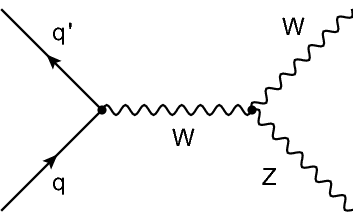
\includegraphics[width=0.3\linewidth]{6_Search/Figures/Feynman/WZa}
	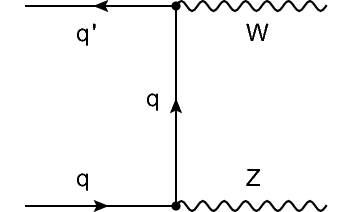
\includegraphics[width=0.3\linewidth]{6_Search/Figures/Feynman/WZb}
	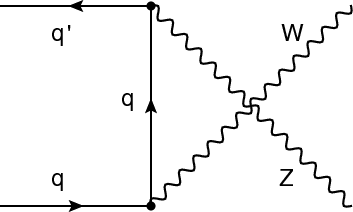
\includegraphics[width=0.3\linewidth]{6_Search/Figures/Feynman/WZc}
	\caption{Leading order Feynmann diagrams for the \WZ\ production in proton collisions. Left: s-channel, middle: t-channel, right: u-channel. Figure taken from~\cite{Khachatryan:2216557}.}
	\label{fig:WZ}
\end{figure}

\begin{figure}[htbp]
	\centering
	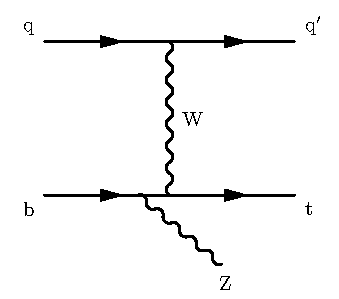
\includegraphics[width=0.3\linewidth]{6_Search/Figures/Feynman/tZq}
	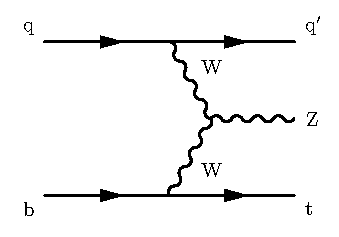
\includegraphics[width=0.3\linewidth]{6_Search/Figures/Feynman/tZq2}
	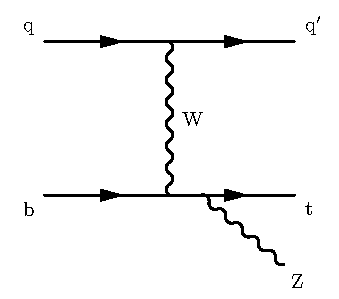
\includegraphics[width=0.3\linewidth]{6_Search/Figures/Feynman/tZq3}
		\caption{Some of the leading order Feynmann diagrams for the \SM\ \tZq\ production in proton collisions. Figure taken from~\cite{CMS-PAS-TOP-16-020}.}
	\label{fig:tZq}
\end{figure}

\begin{figure}[htbp]
	\centering
	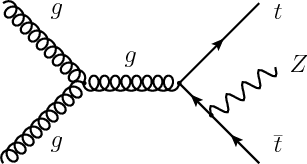
\includegraphics[width=0.3\linewidth]{6_Search/Figures/Feynman/ttZ}
	\caption{Dominant leading order Feynmann diagram for the \ttZ\ production in proton collisions. Figure taken from~\cite{Khachatryan:1712680}.}
	\label{fig:ttZ}
\end{figure}

\begin{figure}[htbp]
	\centering
	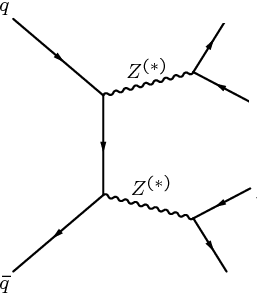
\includegraphics[width=0.3\linewidth]{6_Search/Figures/Feynman/ZZ}
	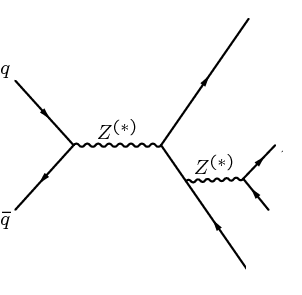
\includegraphics[width=0.3\linewidth]{6_Search/Figures/Feynman/ZZ2}
		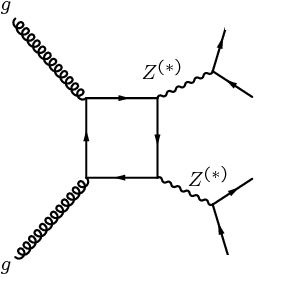
\includegraphics[width=0.3\linewidth]{6_Search/Figures/Feynman/ZZ3}
	\caption{Leading order Feynmann diagram for the \ZZ\ production in proton collisions. Left: t-channel production, middle: s-channel production, right: non-resonant production. The Z$^{(*)}$ notation is used to denote the production of on- and off-shell Z bosons and production of off-shell photons ($\gamma*$). Figure taken from~\cite{Khachatryan:1712680}.}
	\label{fig:ZZ}
\end{figure}
\newpage
\subsection{BDT training in the \STSR\ for the \Zut\ interaction}
\label{sec:BDTSTSRZUT}
Since in the \STSR\, the single top quark FCNC signal is expected to have an enhanced discrimination against the background processes compared to the top quark pair FCNC signal,  the BDT is trained solely to enhance the single top quark FCNC signal. The single top quark FCNC signal expects one \Pbottom\ jet (SM b~jet), one lepton (\PW\ lepton ) and missing transverse energy coming from the \SM\ top quark decay (SM top quark). Furthermore, two leptons from the \PZ\ boson decay are expected. 

The variables used to reconstruct the multivariate discriminator are chosen based on the differences expected between signal and background. For the \STSR, the main backgrounds are the \SM\ tZq, \WZ+jets, and \ZZ\ processes.  The events originating from the \WZ+jet process, are entering the \STSR\ due to a b~jet produced by gluon splitting or the light-flavour jets that are mis-tagged as b~jets.  The SM \tZq\ is entering the \STSR\ when one jets is missing from the reconstruction. The \ZZ\ process is entering the analysis when one  jet is missing from the reconstruction and the other is (mis-)tagged as a b~jet or when one of the four leptons is missing from the reconstruction.  

 The \WZ+jets and \ZZ\ processes do not contain a top quark, while for the \SM\ tZq the reconstructed \SM\ top quark can lose energy via the radiated \PZ\ boson. Therefore variables related to the properties of the top decay through the Wtb vertex are studied for their discriminating power.  The pseudorapidity of the SM top quark $\eta(\mathrm{\SM\ top})$ as well as the invariant mass of the lepton arising from the \PW\ boson $\mathrm{l}_{\PW}$ and the \SM\ b jet, are used as discriminating variables. The distribution of the  pseudorapidity of the SM top quark peaks at zero for the single top quark FCNC signal, while the distribution is broader for the background contributions. The distribution of the invariant mass of the lepton arising from the \PW\ boson and the \SM\ b~jet peaks at around 100~\GeV\ for signal and background, where the distribution of the background processes has a longer tail. Additionally, the difference in $\phi$ between the \PW\ lepton and the SM b~jet $\Delta \phi(\Plepton_{\PW},b)$ peaks around $\pm 1$ for signal, while for background this is at $\pm 3$. This indicates that for background, the  W lepton and the SM b jet are not necessarily coming from the same object, while for signal these objects are closer together. This is also visible in the distribution of the difference in distance in the $\phi\eta$-plane, $\Delta R(\Plepton_{\PW},b)$, between the W lepton and the SM b jet, where signal is peaking at lower values.
 
    For signal, the lepton assigned to the \PW\ boson should be back-to-back to the \PZ\ boson, this is used by looking at the difference in  $\Delta R$ between the W lepton and the Z boson $\Delta R(Z,\Plepton_{\PW})$, which peaks at three for the single top quark FCNC signal  distribution. For the  background processes the peak  in the distribution is broader. For the signal, the jet with the highest transverse momentum is expected to be the b~jet. This jet is expected to have a high transverse momentum. For this reason, the CSVv2 discriminant of the jet with the highest \pt\ (CSVv2 jet $\pt^{\mathrm{max}}$) is used as discriminating variable, peaking at one for the single top quark FCNC signal  process and resembling a flat distribution for the backgrounds. The disitribution of the scalar sum of the \pt\ of the leptons, H$_{\mathrm{T}}$, is peaking at higher values for the single top quark FCNC signal . Hence, the single top quark FCNC signal  is more transverse than its backgrounds.
    
     Since the up quark is a valence quark for the proton, while the anti-up quark is a sea quark, one expects a charge asymmetry for the production of top and anti-top quarks. This effect is exploited by using 
the charge of the W lepton times the absolute pseudorapidity of the W lepton ($|\eta(\Plepton_{\PW})|\times Q(\Plepton_{\PW})$) and  the \pt\ of the W lepton times its charge ($\pt(\Plepton_{\PW})\times Q(\Plepton_{\PW})$) as discriminating variables. Where the fact that the single top quark FCNC signal is more transverse than it backgrounds is used for the combination $|\eta(\Plepton_{\PW})|\times Q(\Plepton_{\PW})$. In the combination $\pt(\Plepton_{\PW})\times Q(\Plepton_{\PW})$, the fact that the single top quark FCNC signal is expecting a high-\pt\ prompt lepton is used. 

 The distributions of the variables are shown in \fig{fig:singletopZutnormalized} for the  \mumumu\ lepton channel, the distributions for the other three-lepton channels can be found in \App{app:BDTcorrZutSing}. The correlations between the different variables are shown in \fig{fig:correlationsigzutsingletop}.
 
  The correlation between the variables is mostly small, and varies from zero to $\sim 60\%$. The most discriminating variable is the distance in the $\phi\eta$-plane between the \PW\ lepton and the SM b jet, followed by the CSVv2 discriminator of the jet with the highest \pt. On the third place is the invariant mass of the \PW\ lepton and \SM\ b jet system. % harde cut off in dR op 3.14 is omdat phi maar een max vercshil van pi heeft
\begin{figure}[htbp]
	\centering
	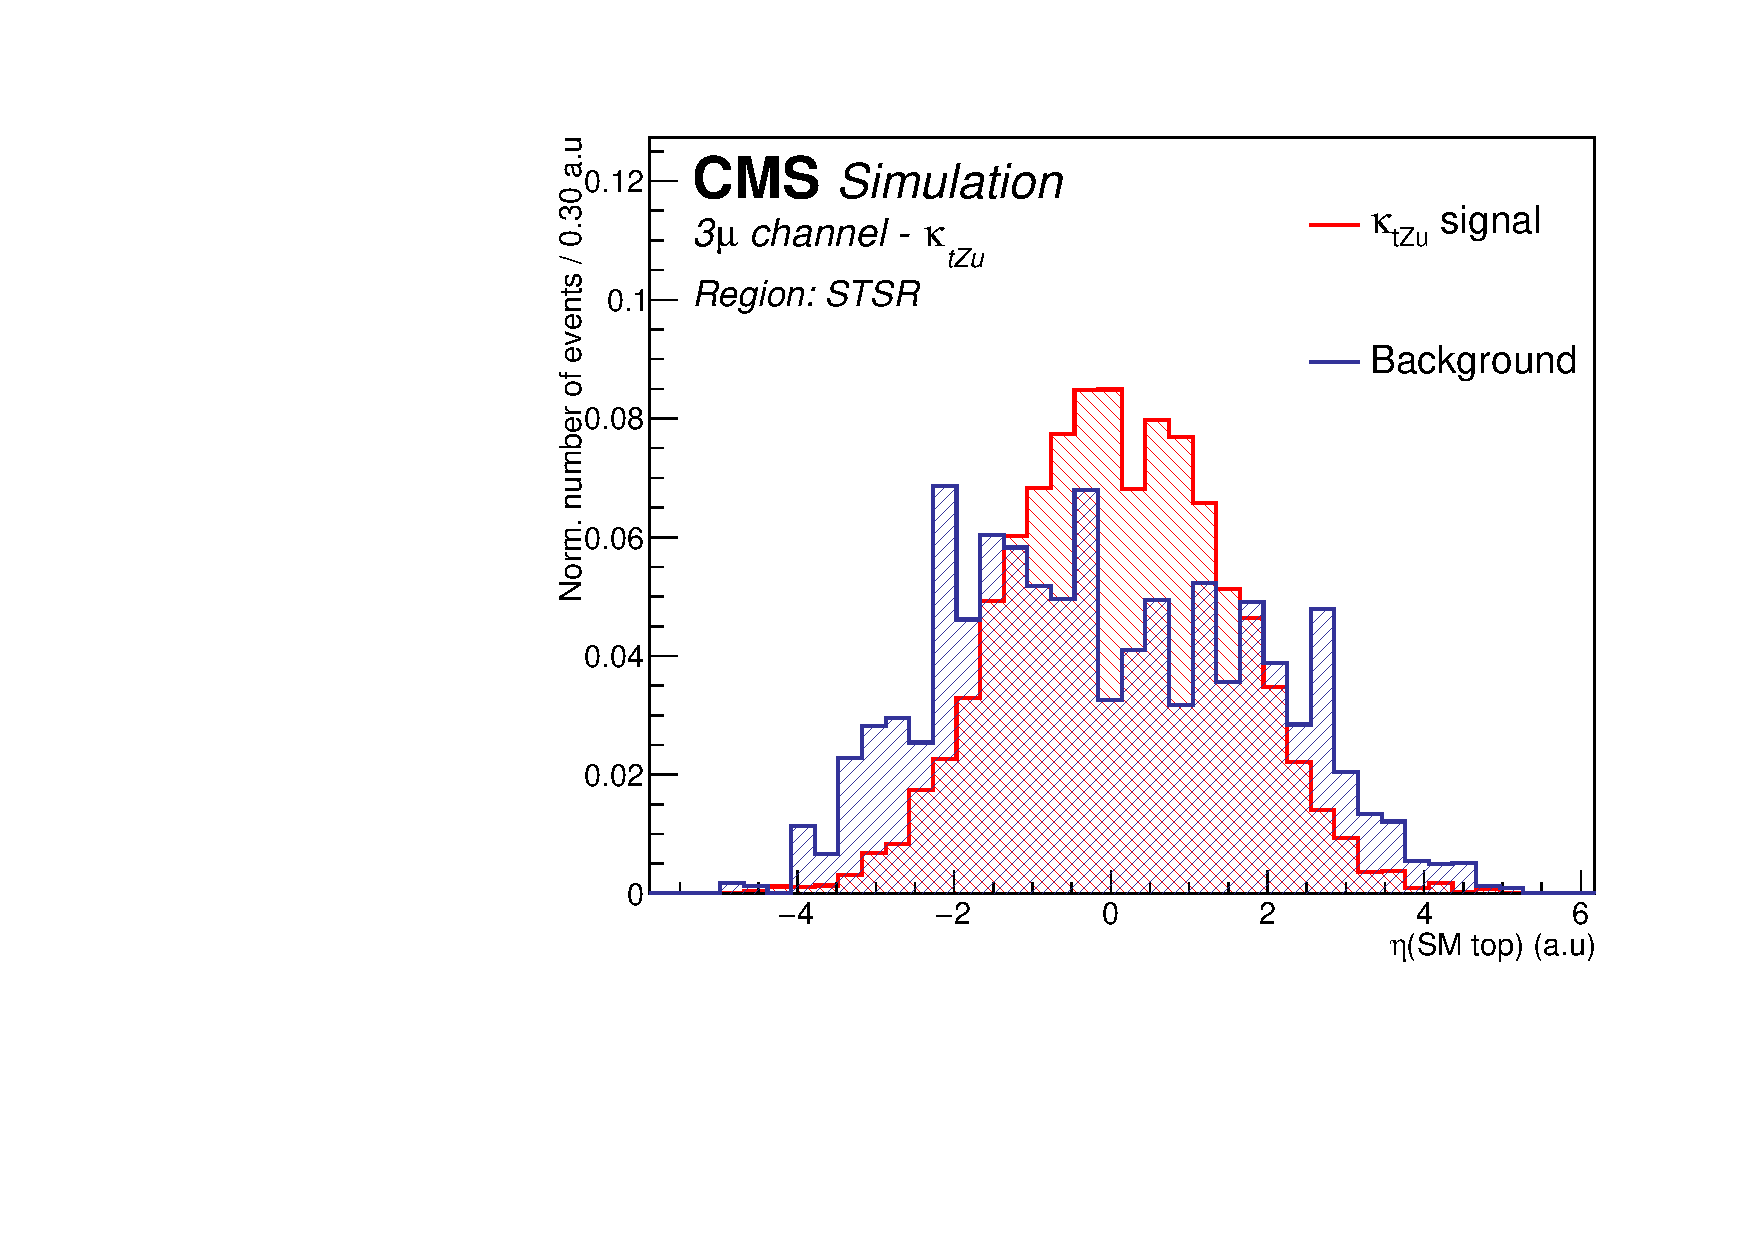
\includegraphics[width=0.3\linewidth]{6_Search/Figures/PlotsTechnics/SMtopetaZutsingletopuuu_norm}
	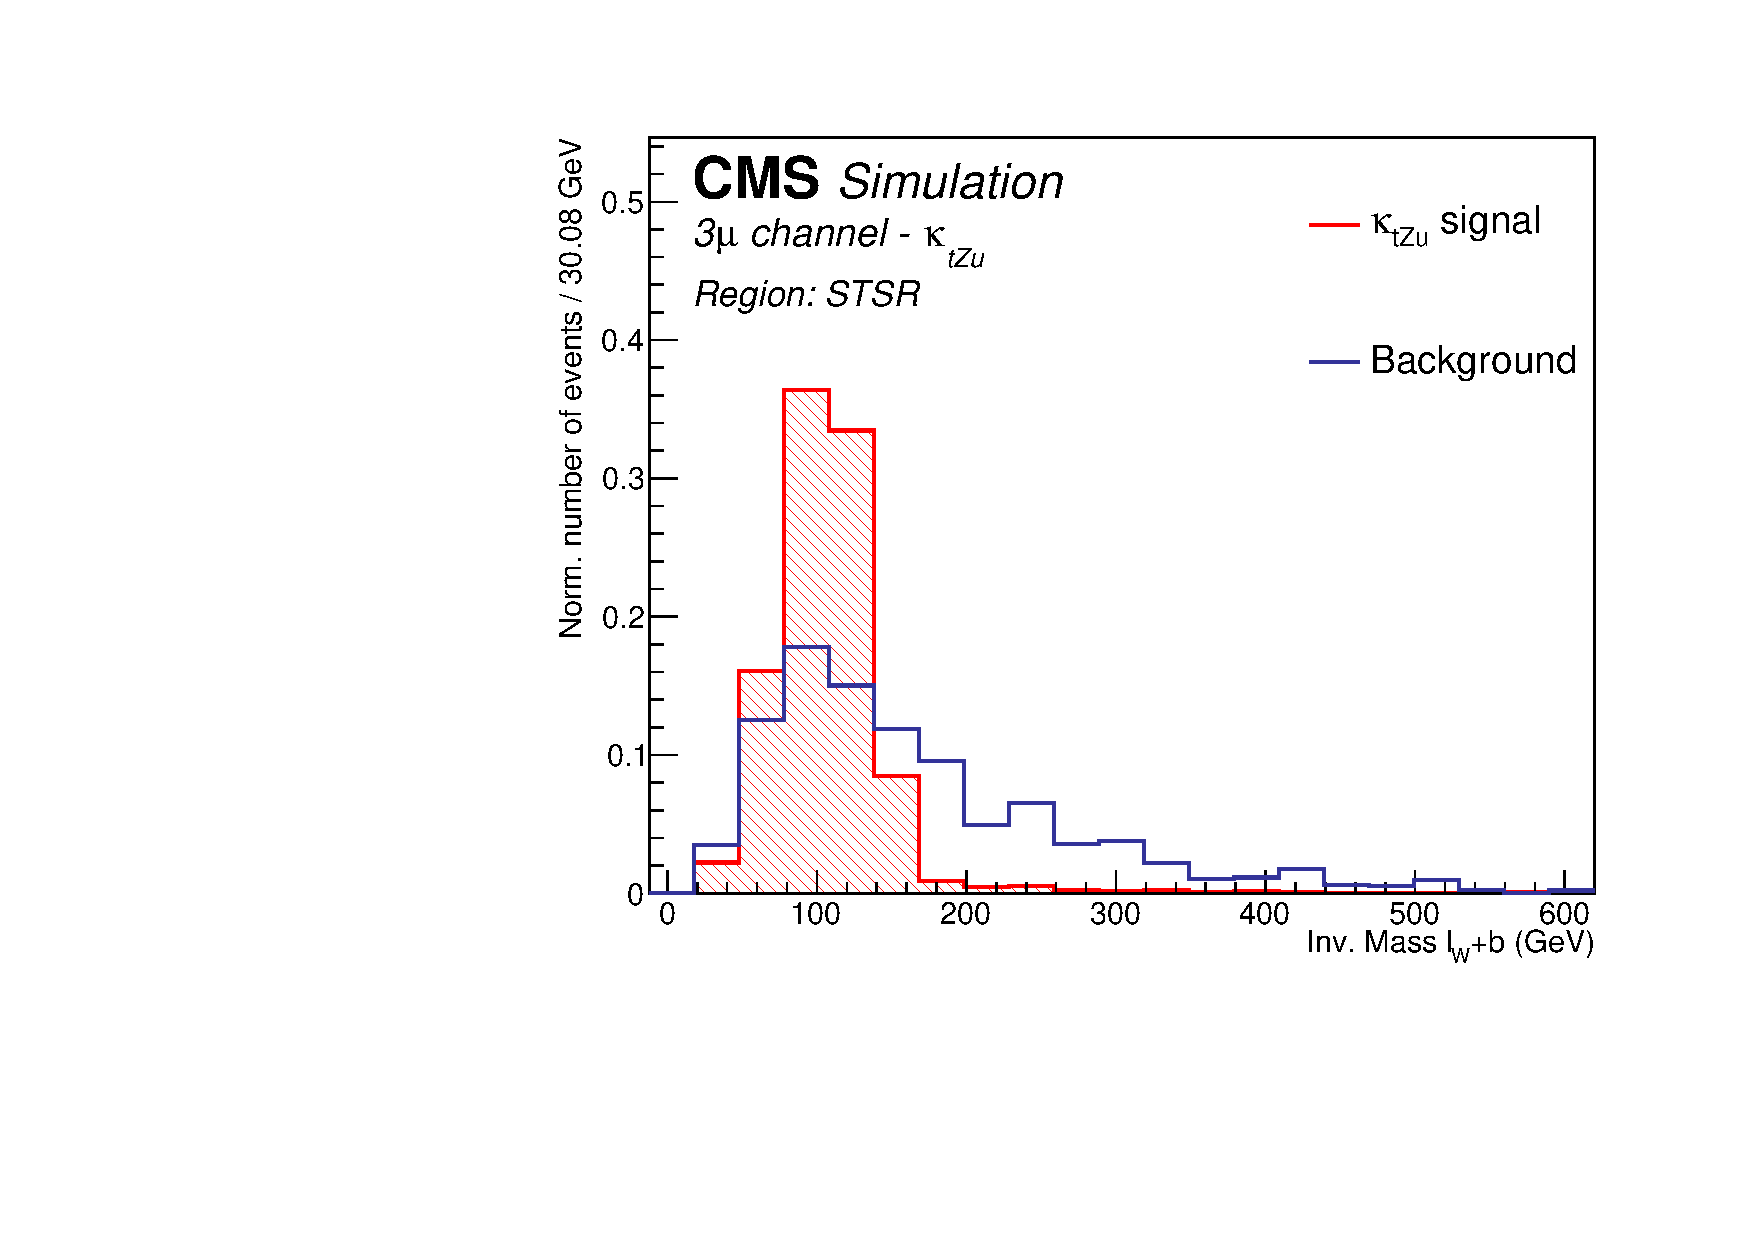
\includegraphics[width=0.3\linewidth]{6_Search/Figures/PlotsTechnics/mlbZutsingletopuuu_norm}
	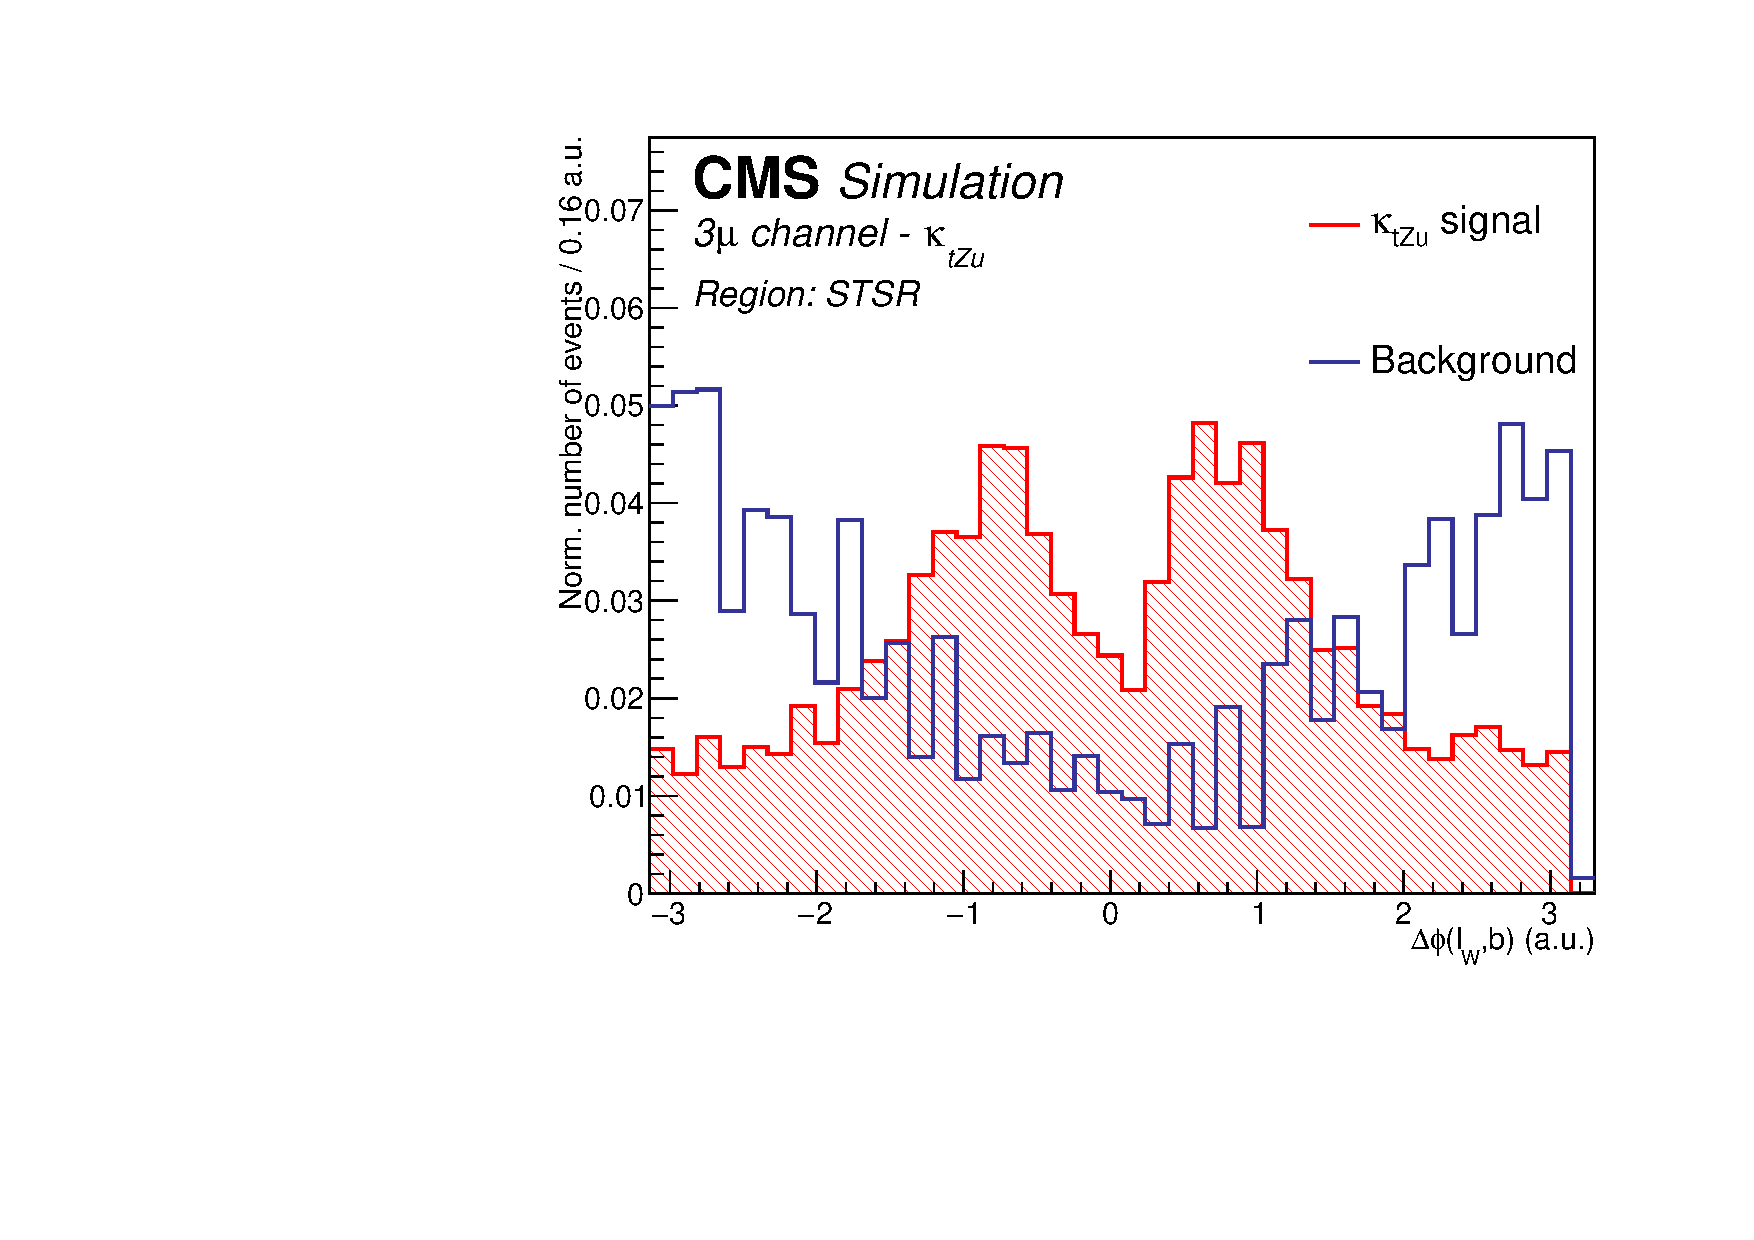
\includegraphics[width=0.3\linewidth]{6_Search/Figures/PlotsTechnics/dPhiWlepbZutsingletopuuu_norm}
	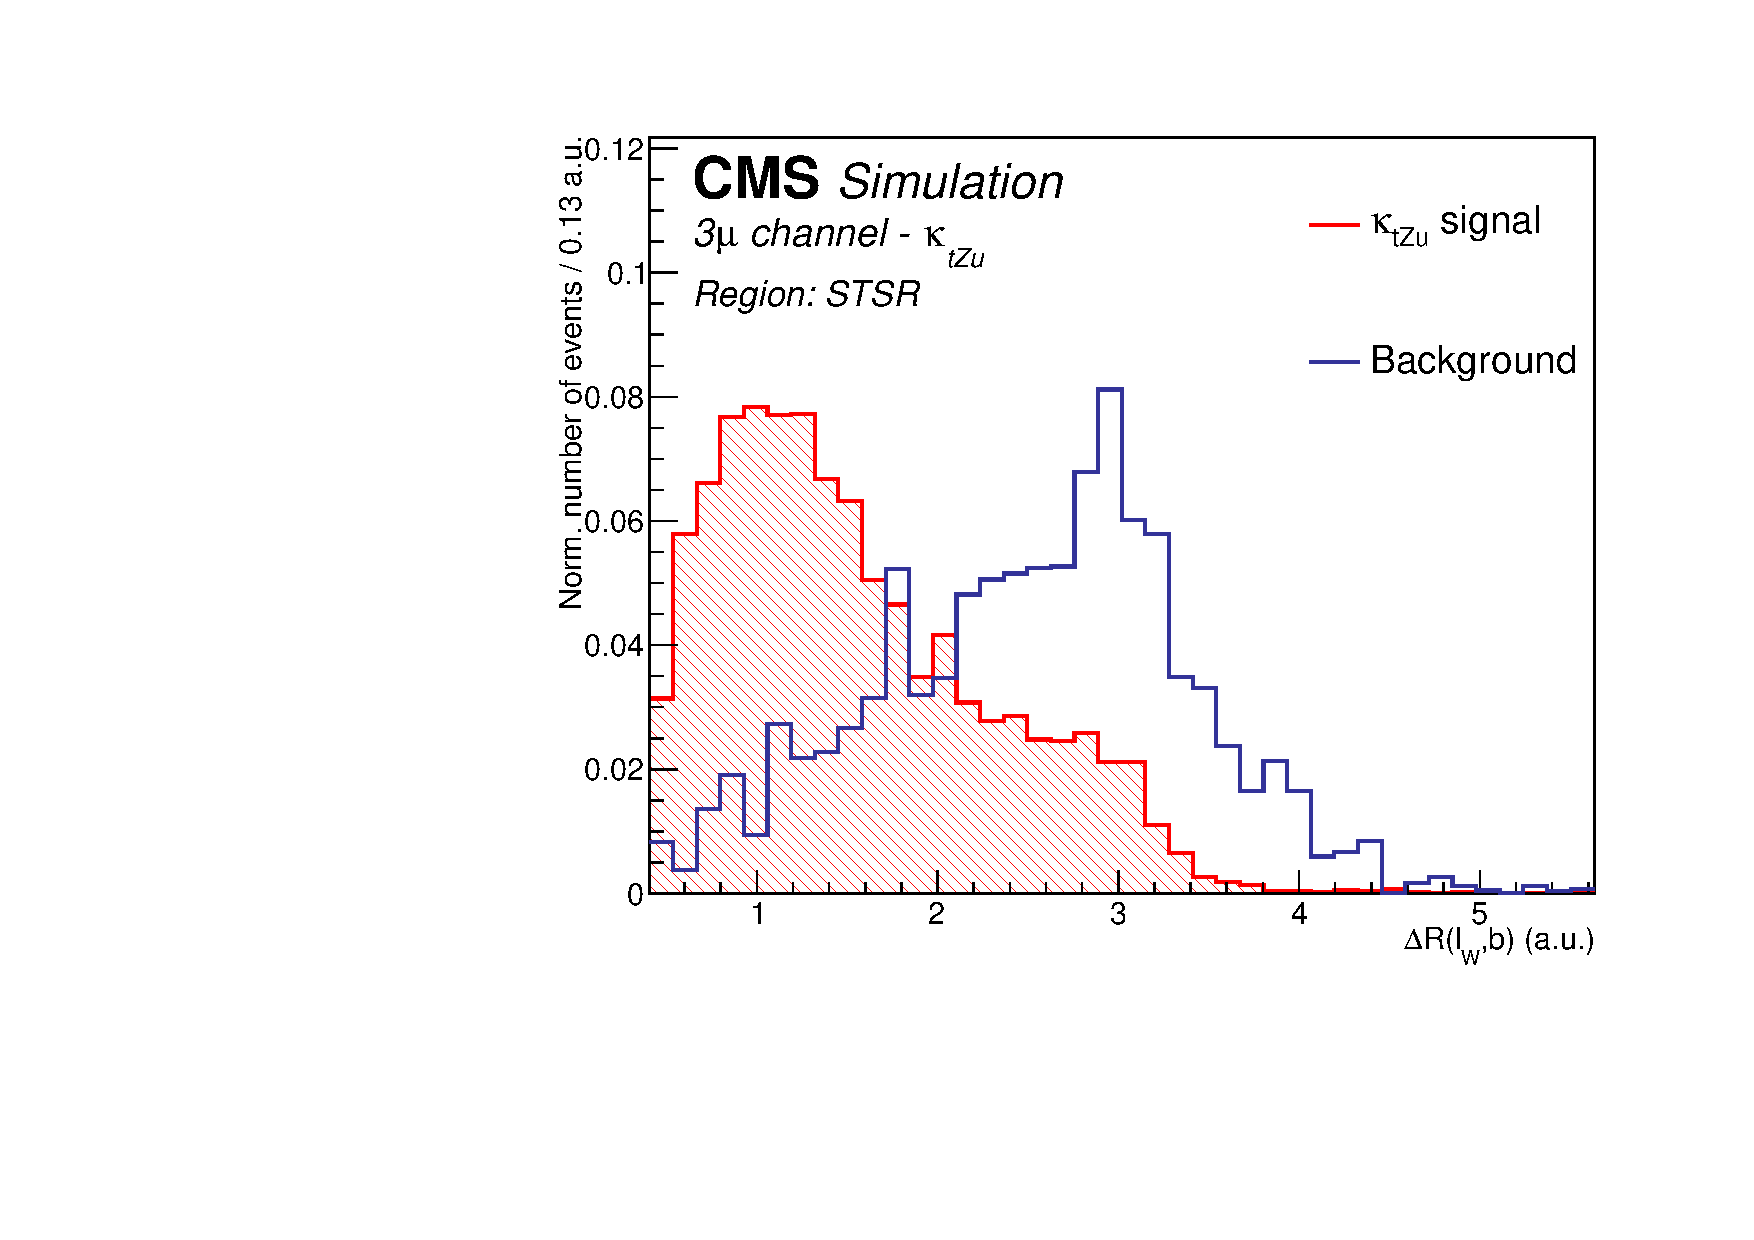
\includegraphics[width=0.3\linewidth]{6_Search/Figures/PlotsTechnics/dRWlepbZutsingletopuuu_norm}
		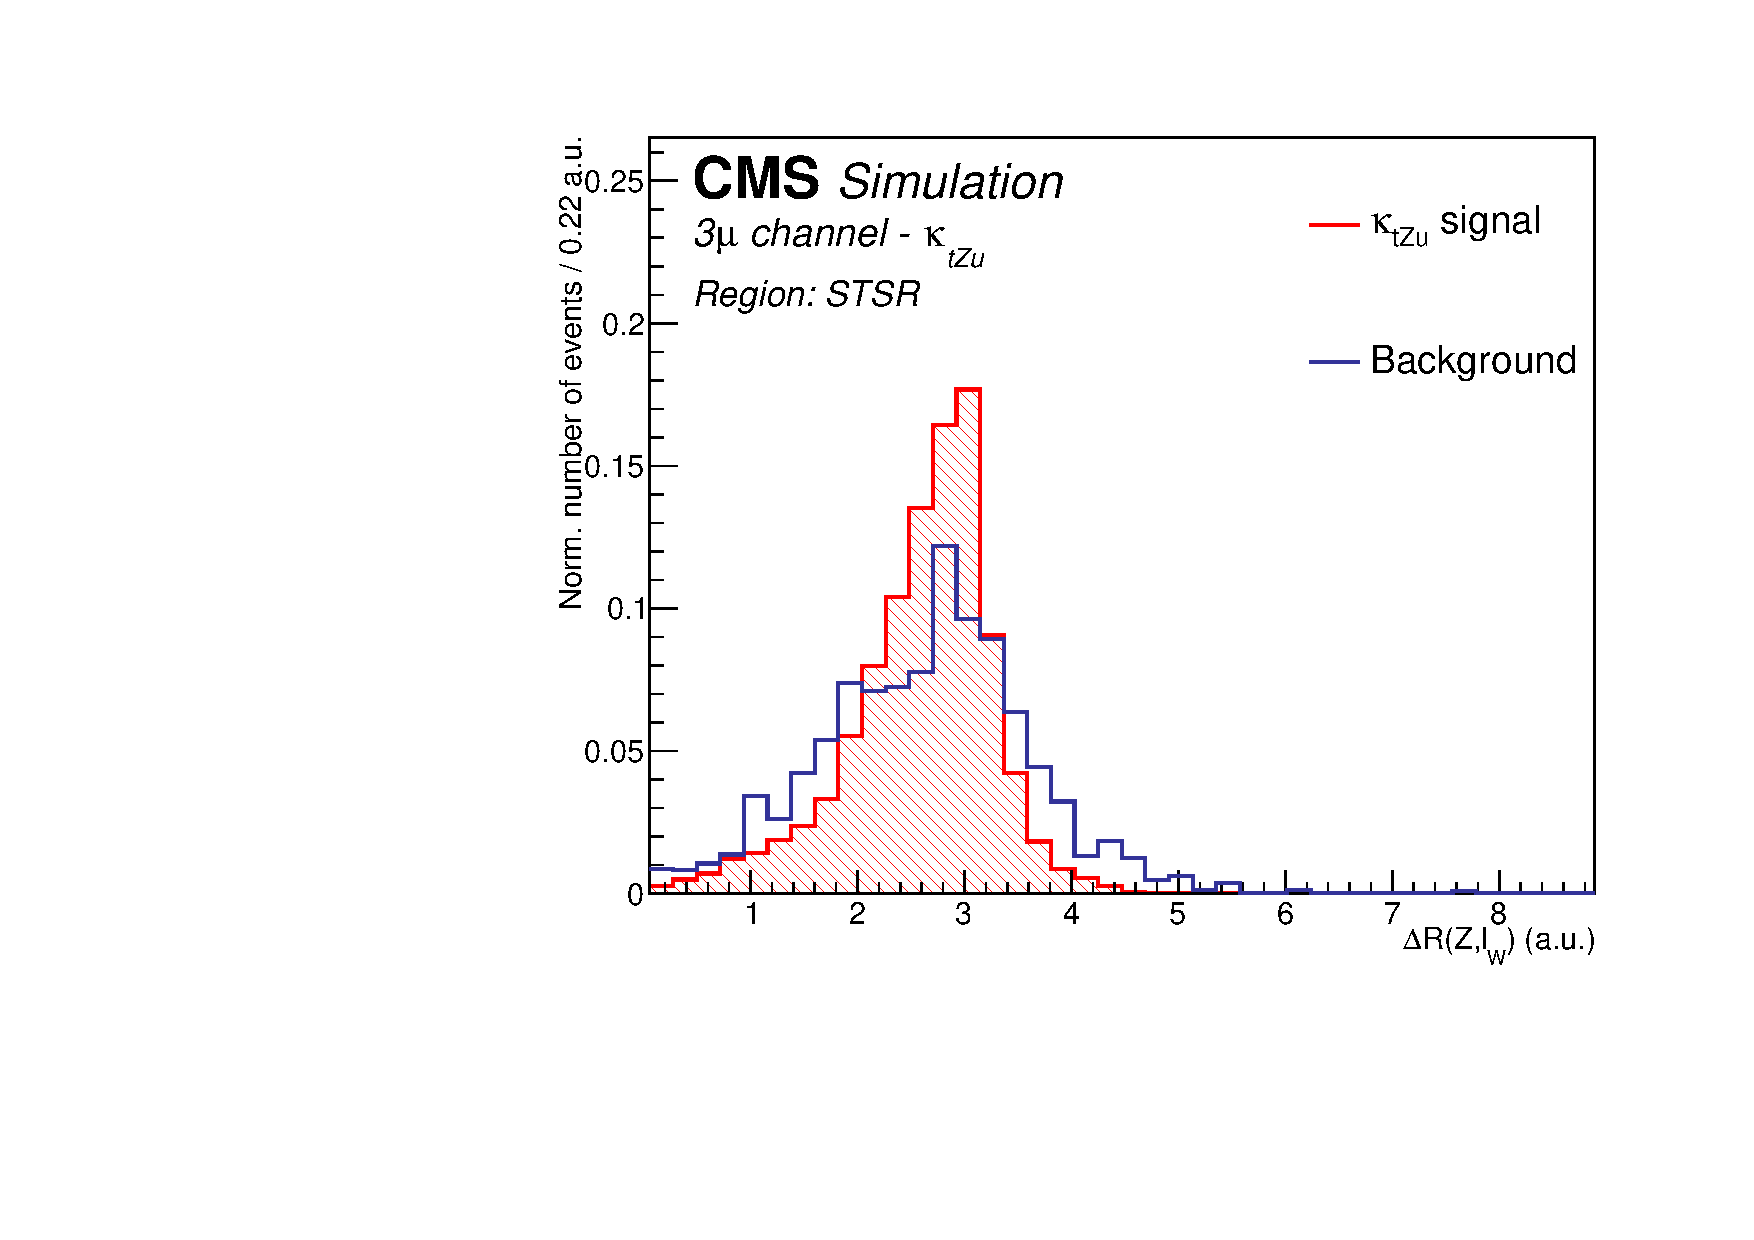
\includegraphics[width=0.3\linewidth]{6_Search/Figures/PlotsTechnics/dRZWlepZutsingletopuuu_norm}
	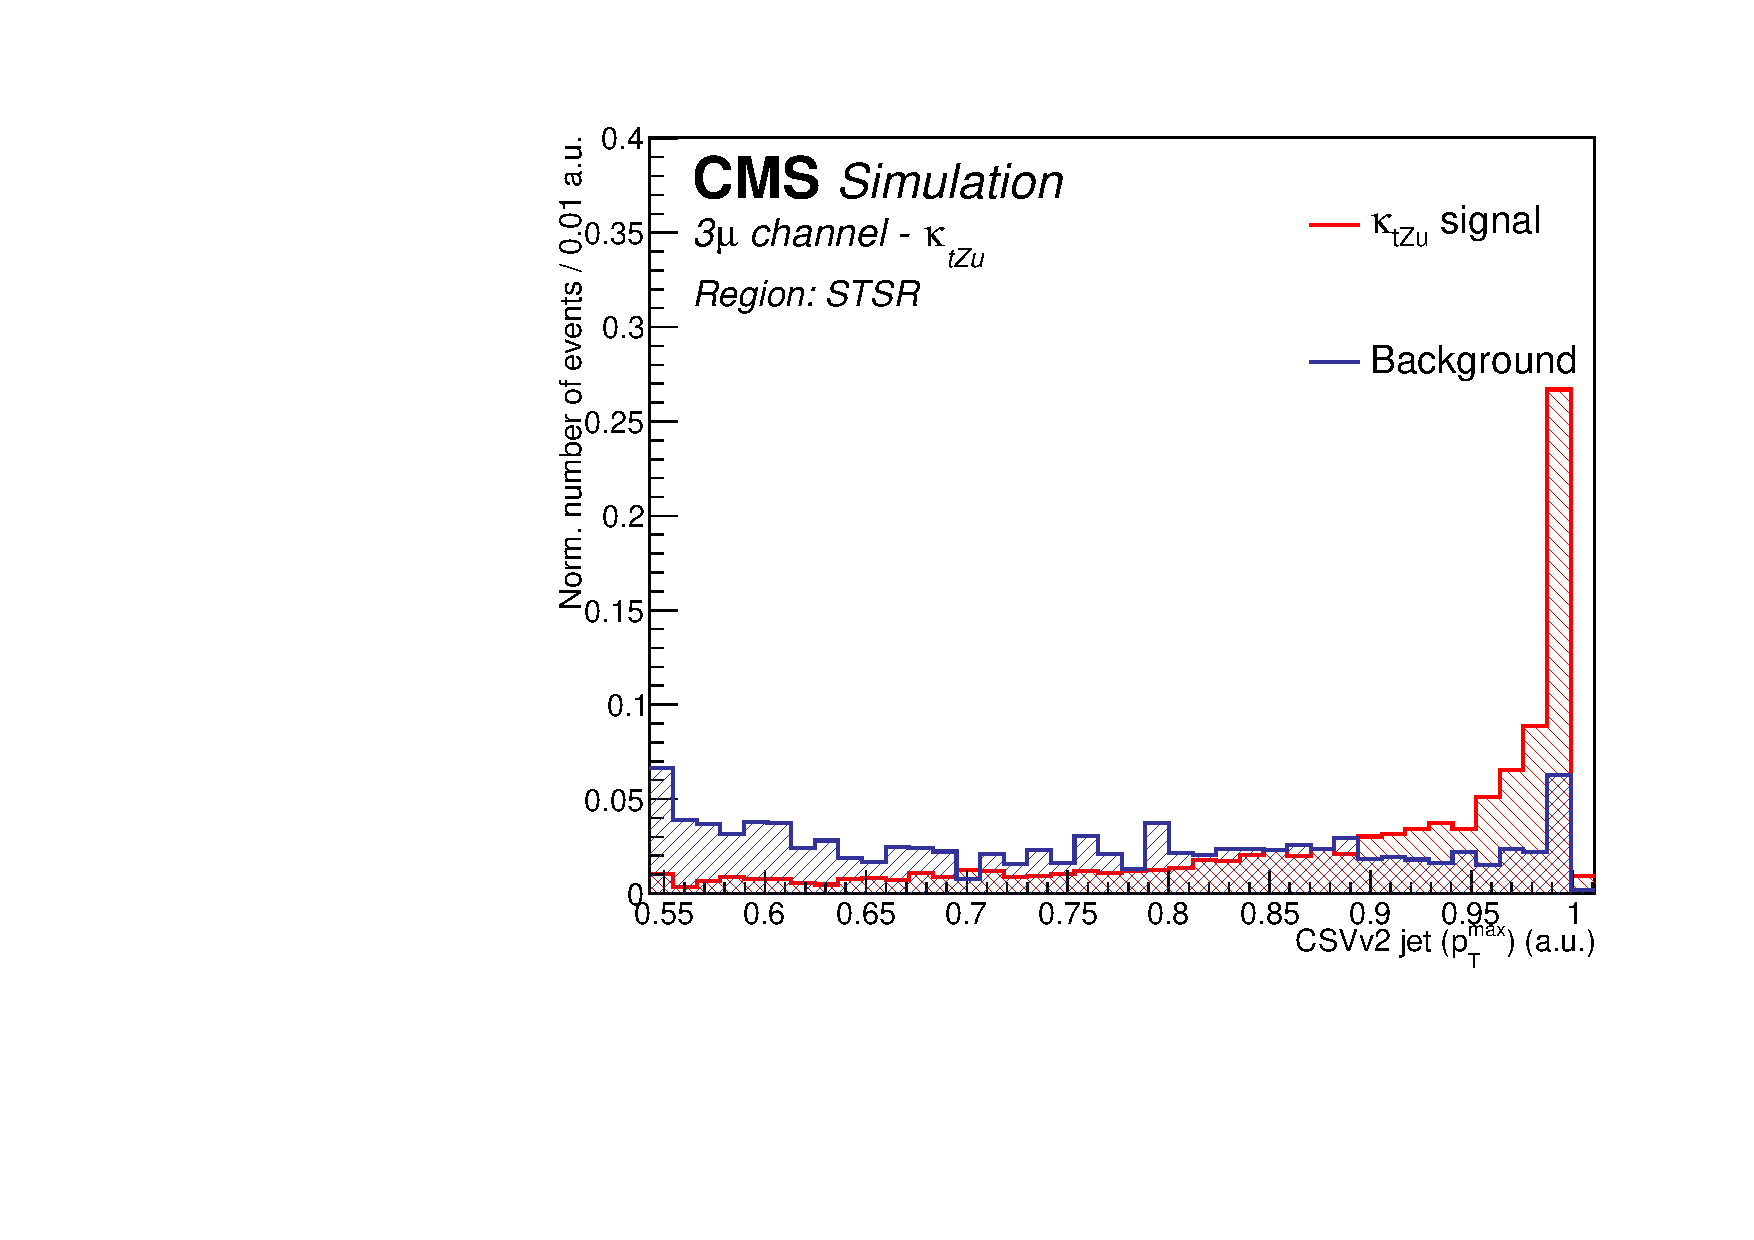
\includegraphics[width=0.3\linewidth]{6_Search/Figures/PlotsTechnics/bdiscCSVv2_jet_0Zutsingletopuuu_norm}
		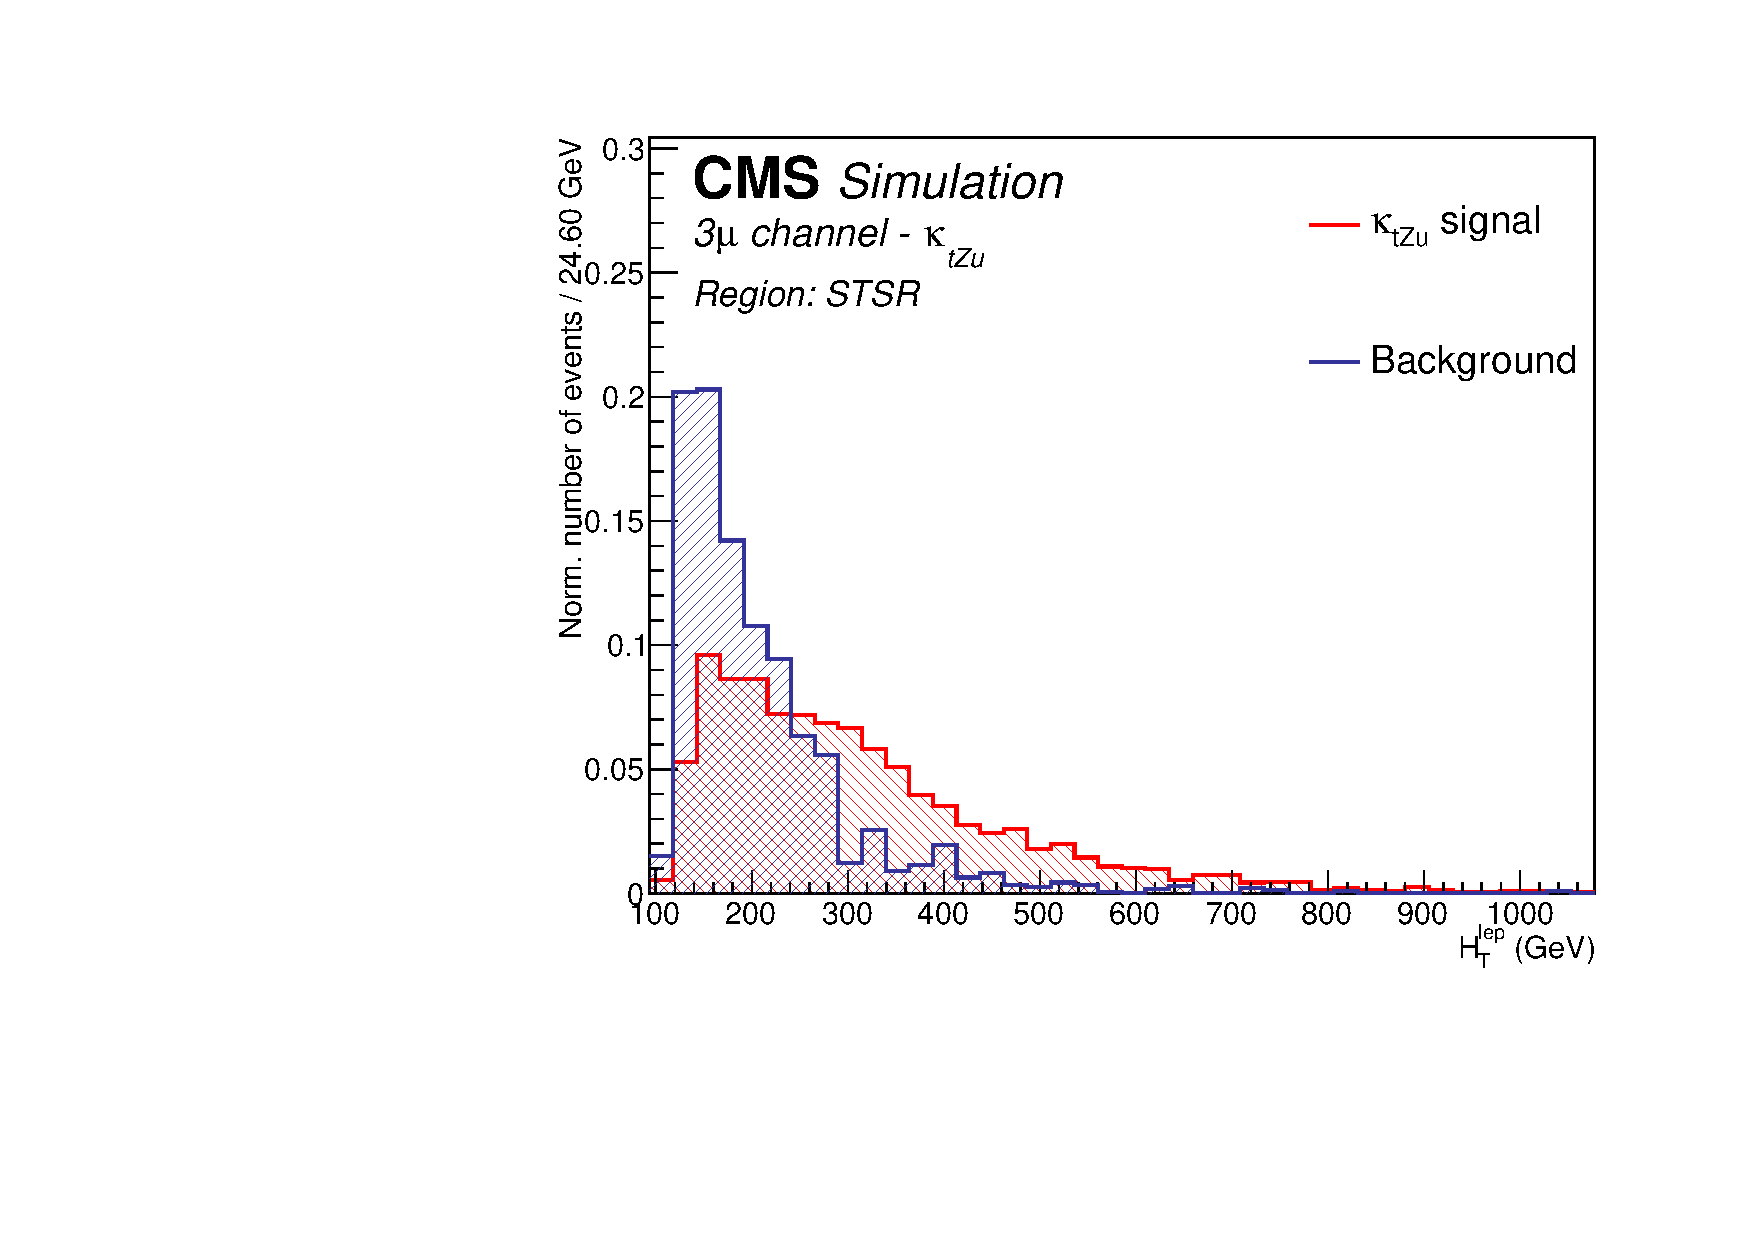
\includegraphics[width=0.3\linewidth]{6_Search/Figures/PlotsTechnics/TotalHt_lepZutsingletopuuu_norm}
	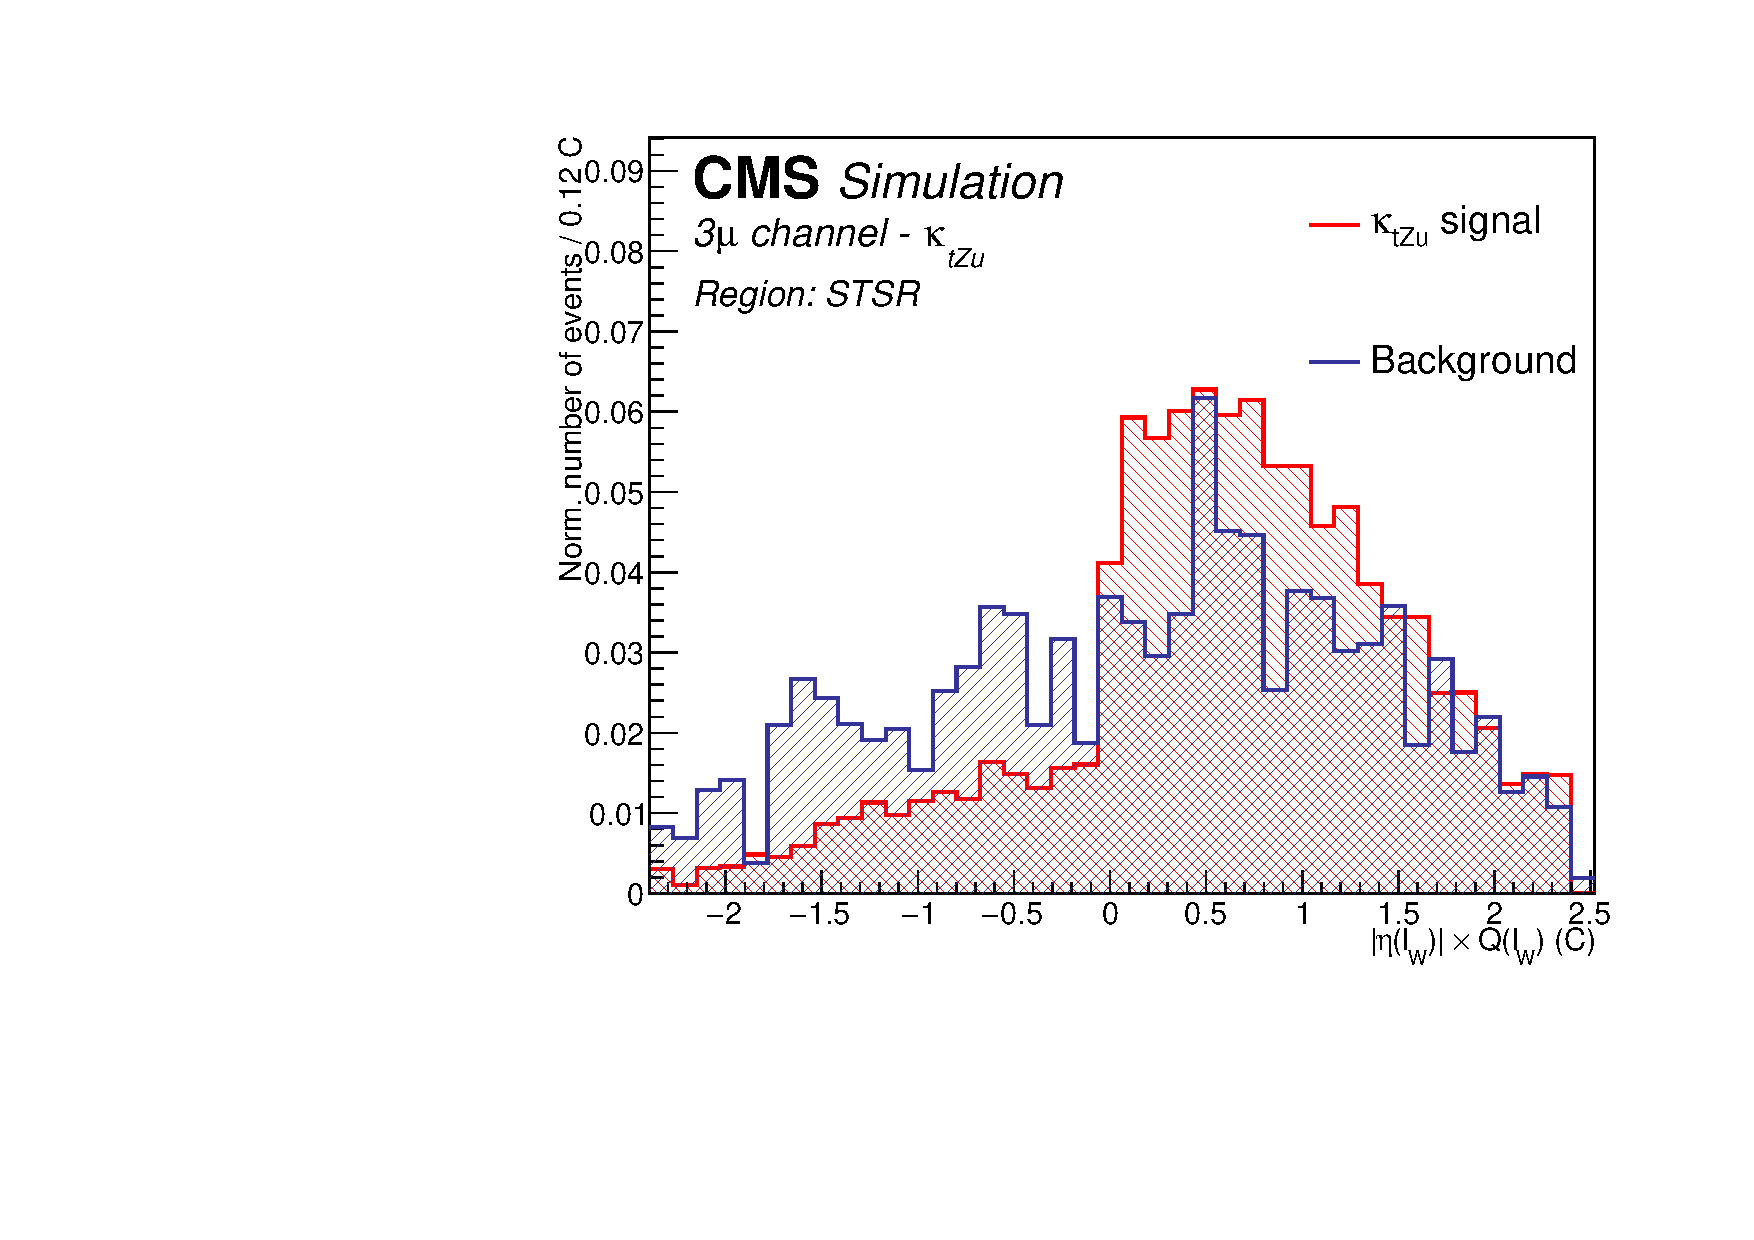
\includegraphics[width=0.3\linewidth]{6_Search/Figures/PlotsTechnics/charge_asymZutsingletopuuu_norm}
			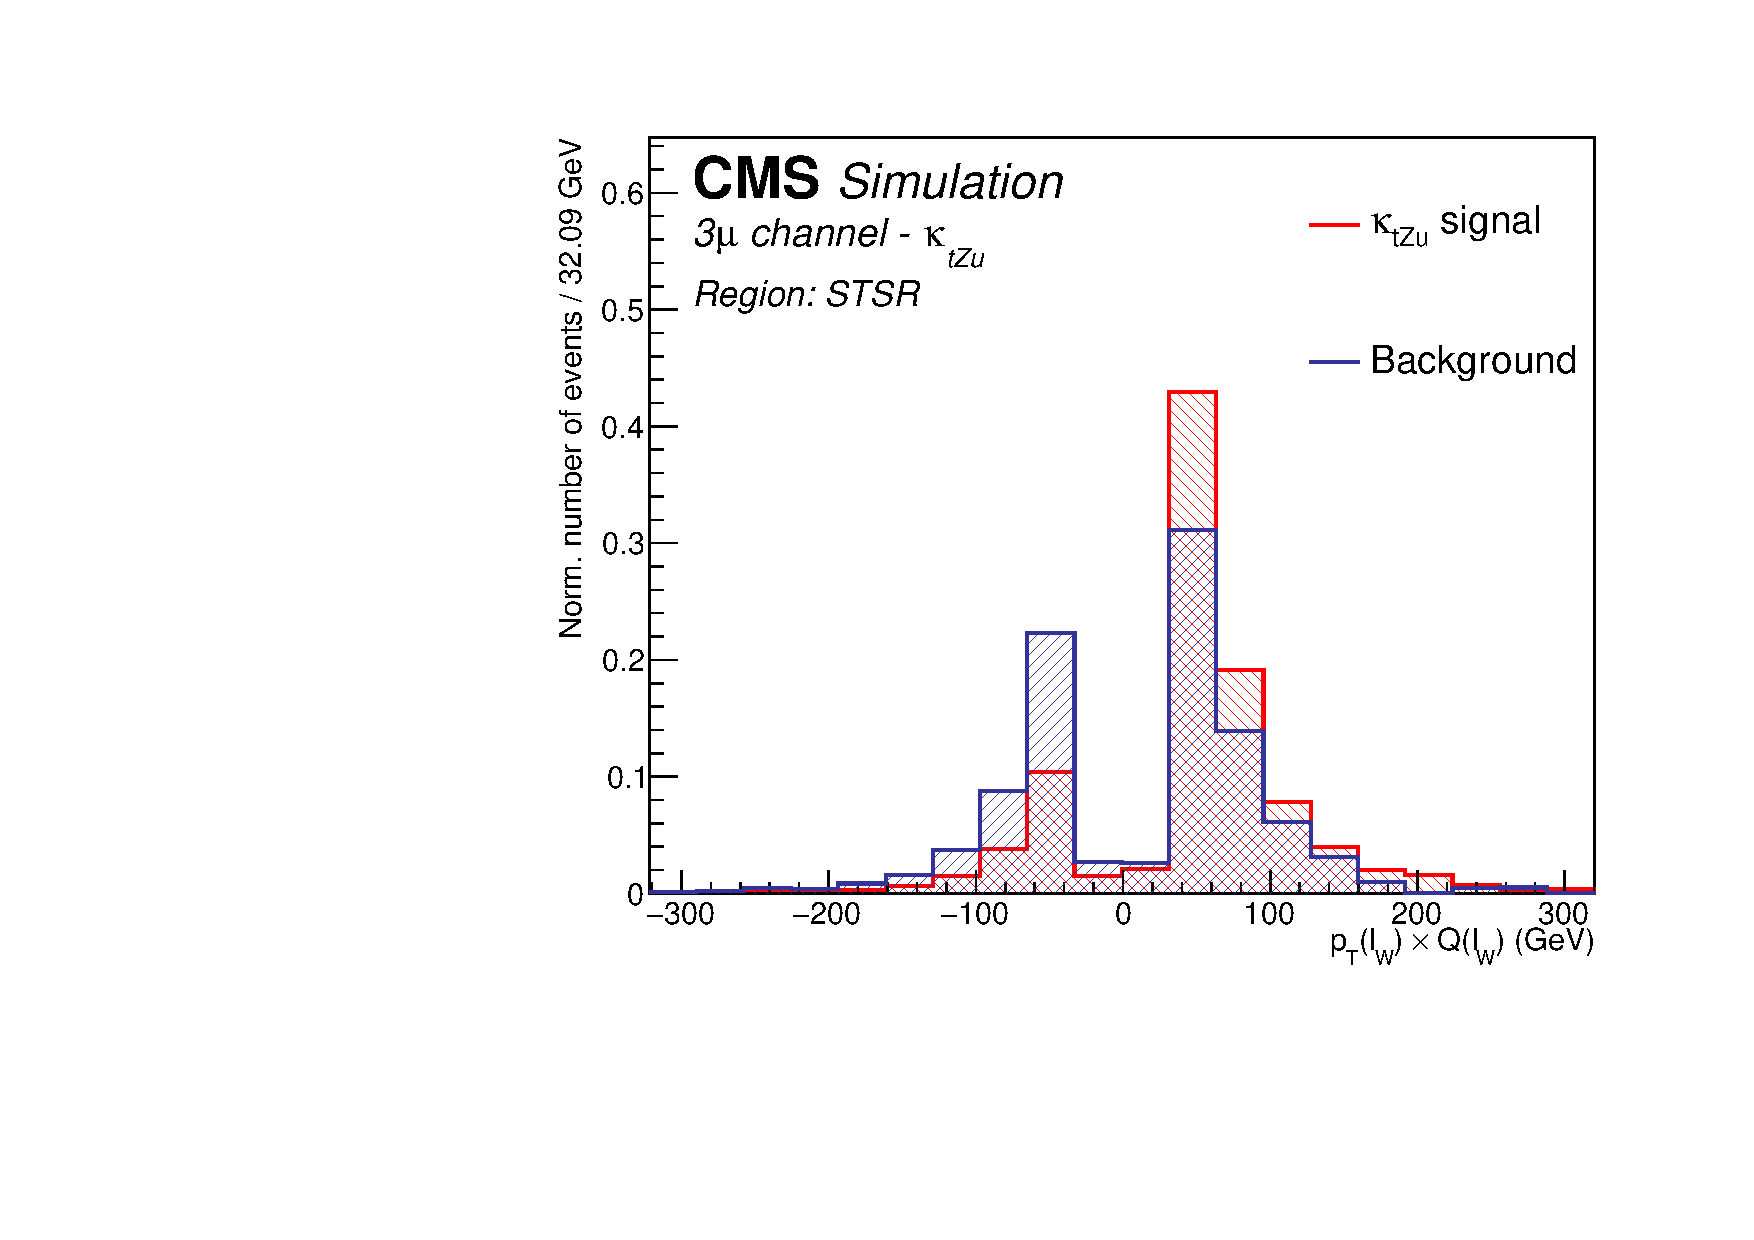
\includegraphics[width=0.3\linewidth]{6_Search/Figures/PlotsTechnics/ptWQZutsingletopuuu_norm}
	\caption{The normalised distributions of the input variables for reconstructing the multivariate discriminator in the \STSR\ for the \Zut\ vertex for the \mumumu\ channel. The contribution of the \NPL\ background is not included. }
	\label{fig:singletopZutnormalized}
\end{figure}
\begin{figure}[htbp]
	\centering
	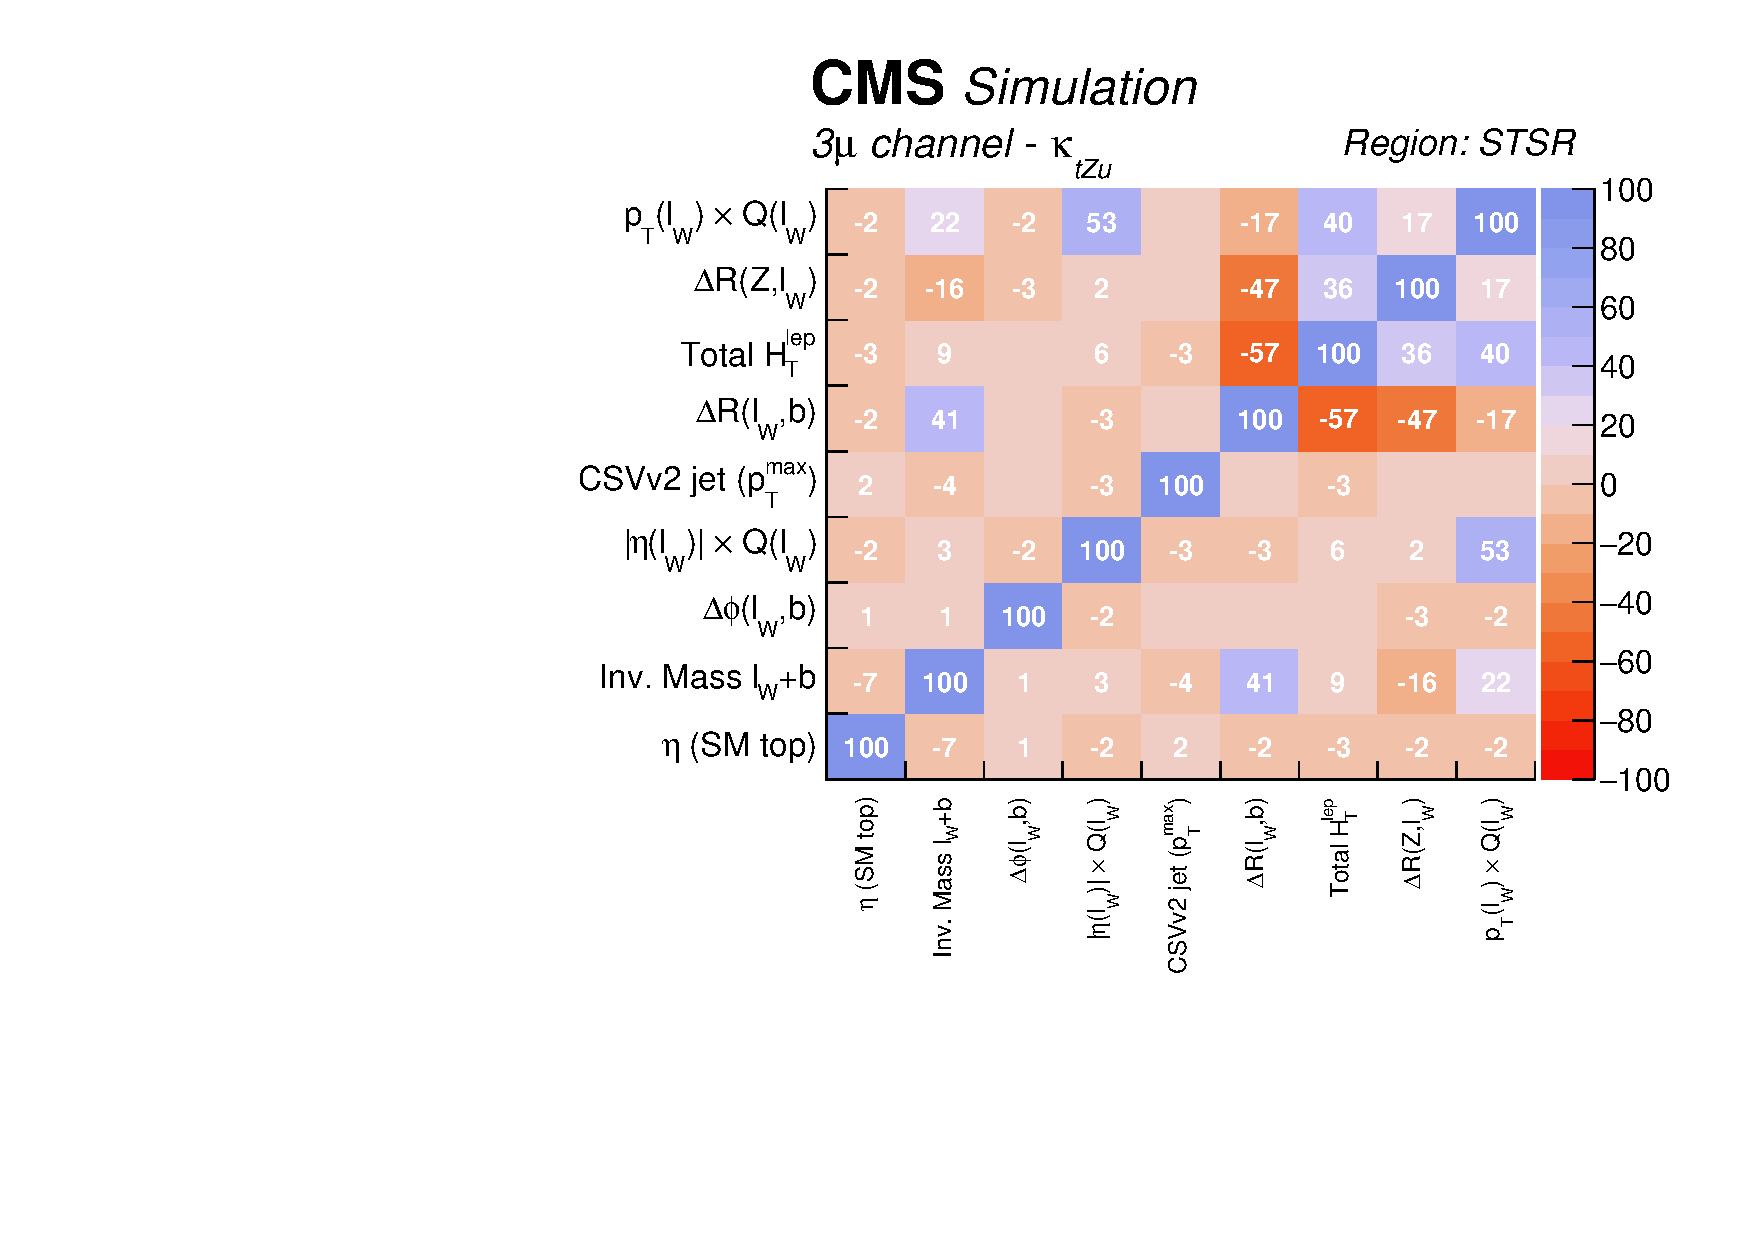
\includegraphics[width=0.49\linewidth]{6_Search/Figures/PlotsTechnics/correlationsigZutsingletopuuu}
	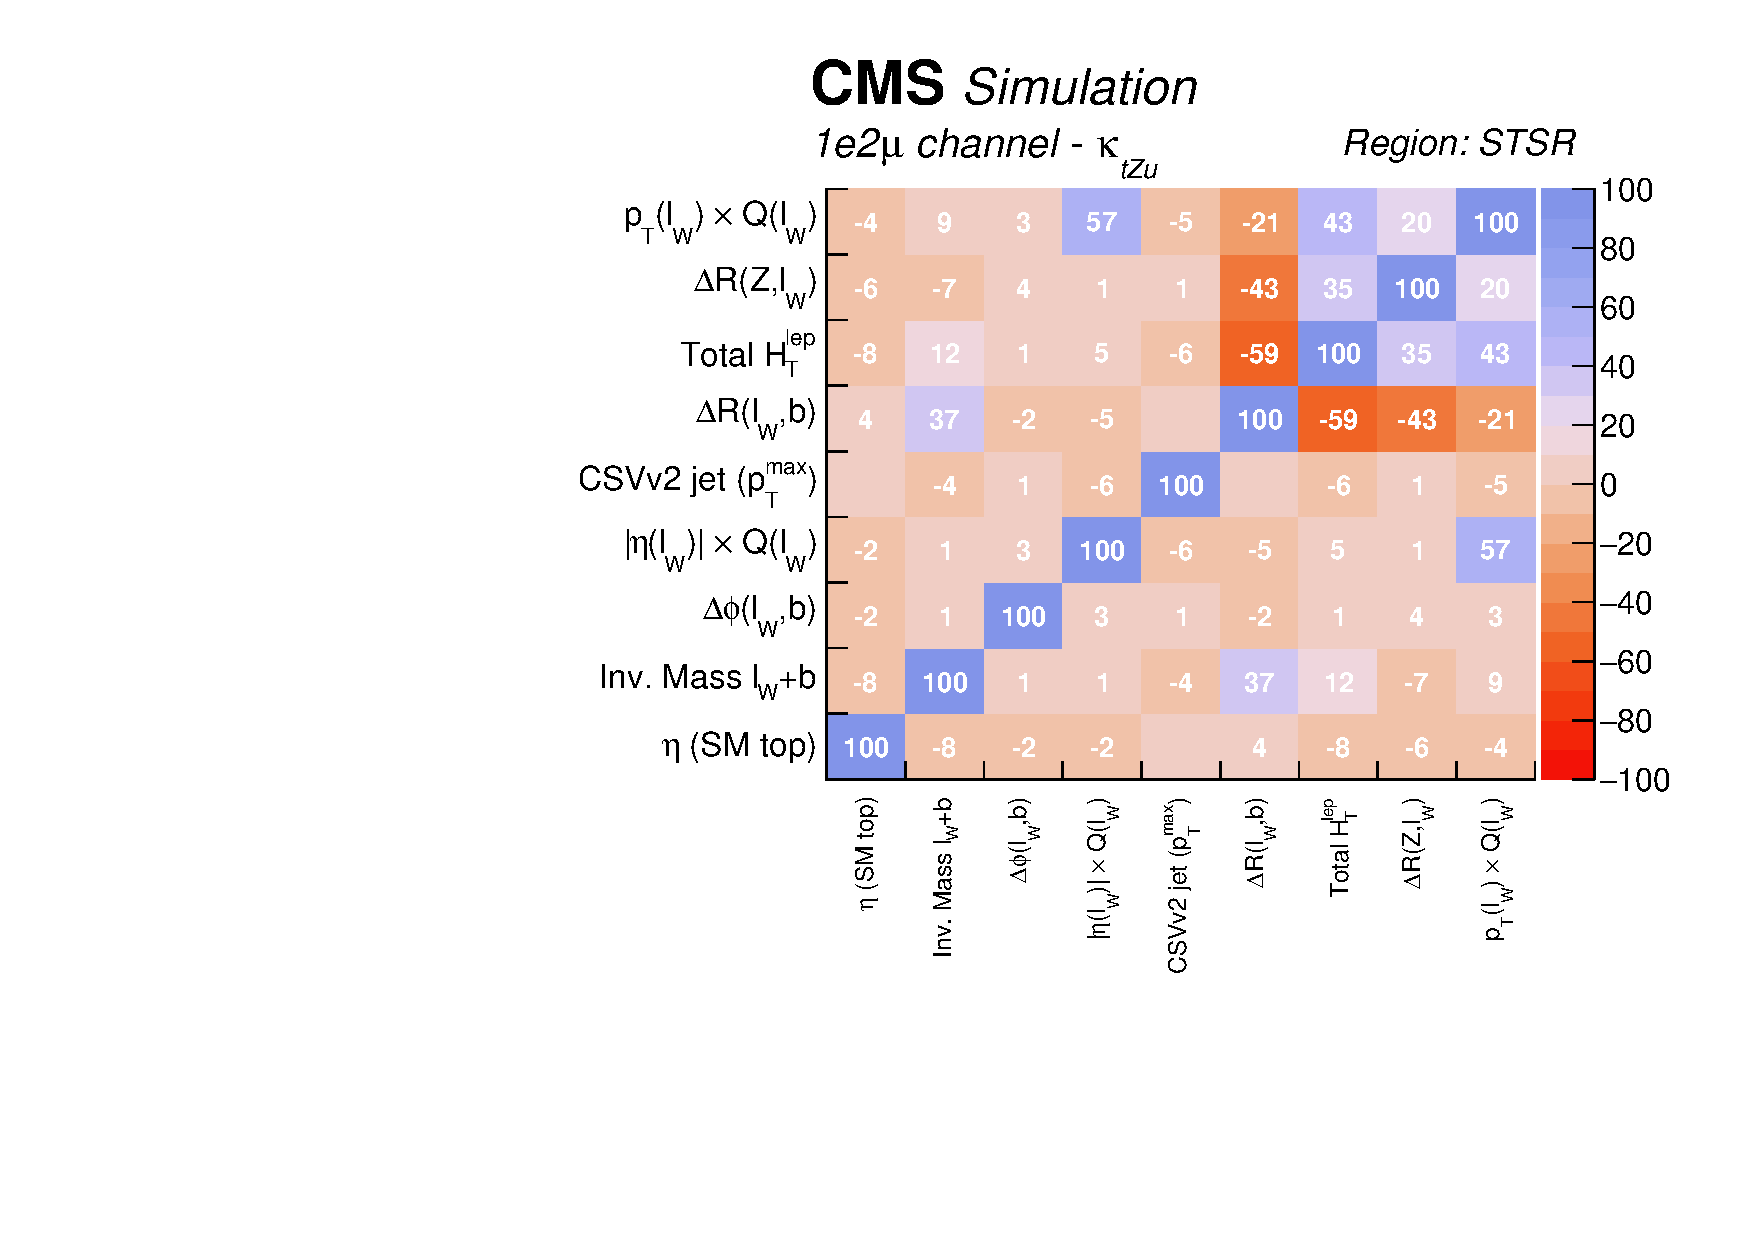
\includegraphics[width=0.49\linewidth]{6_Search/Figures/PlotsTechnics/correlationsigZutsingletopuue}
	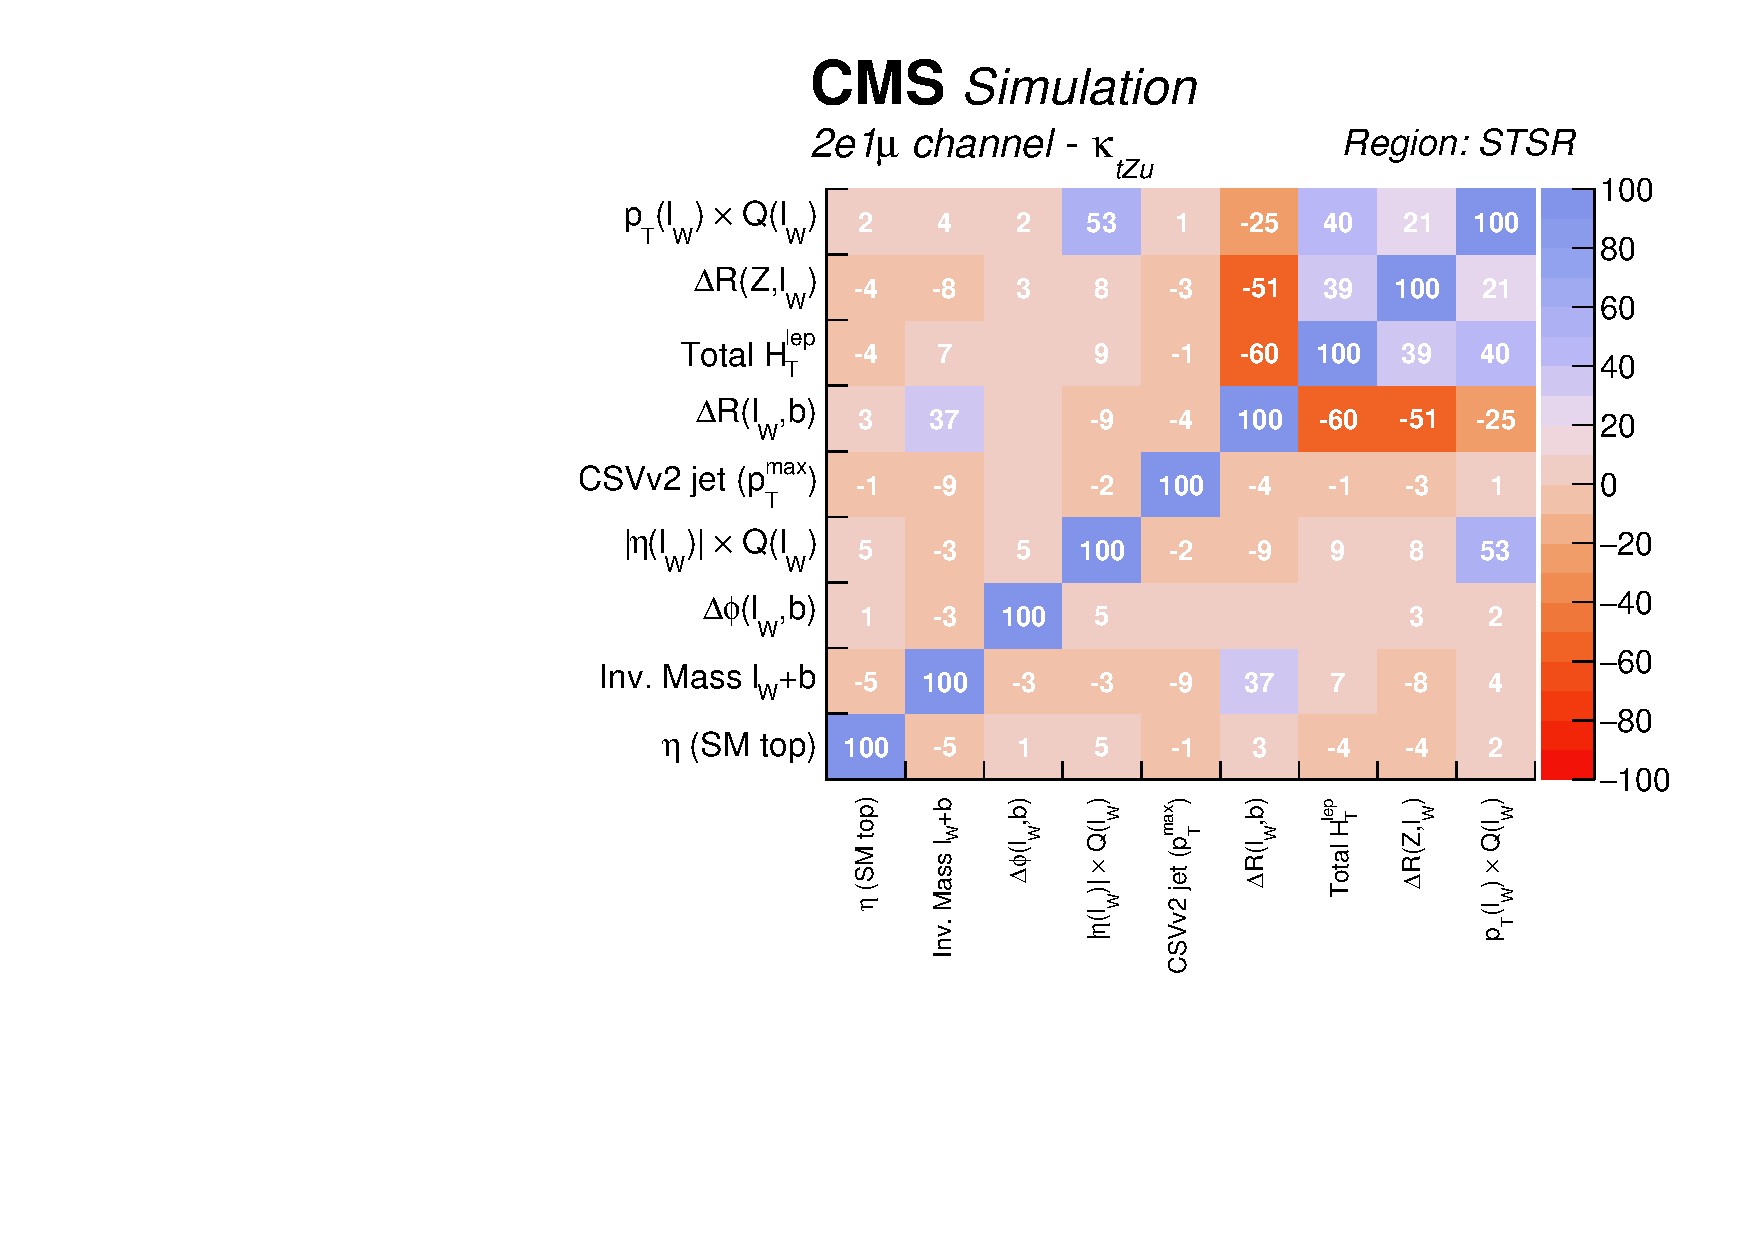
\includegraphics[width=0.49\linewidth]{6_Search/Figures/PlotsTechnics/correlationsigZutsingletopeeu}
	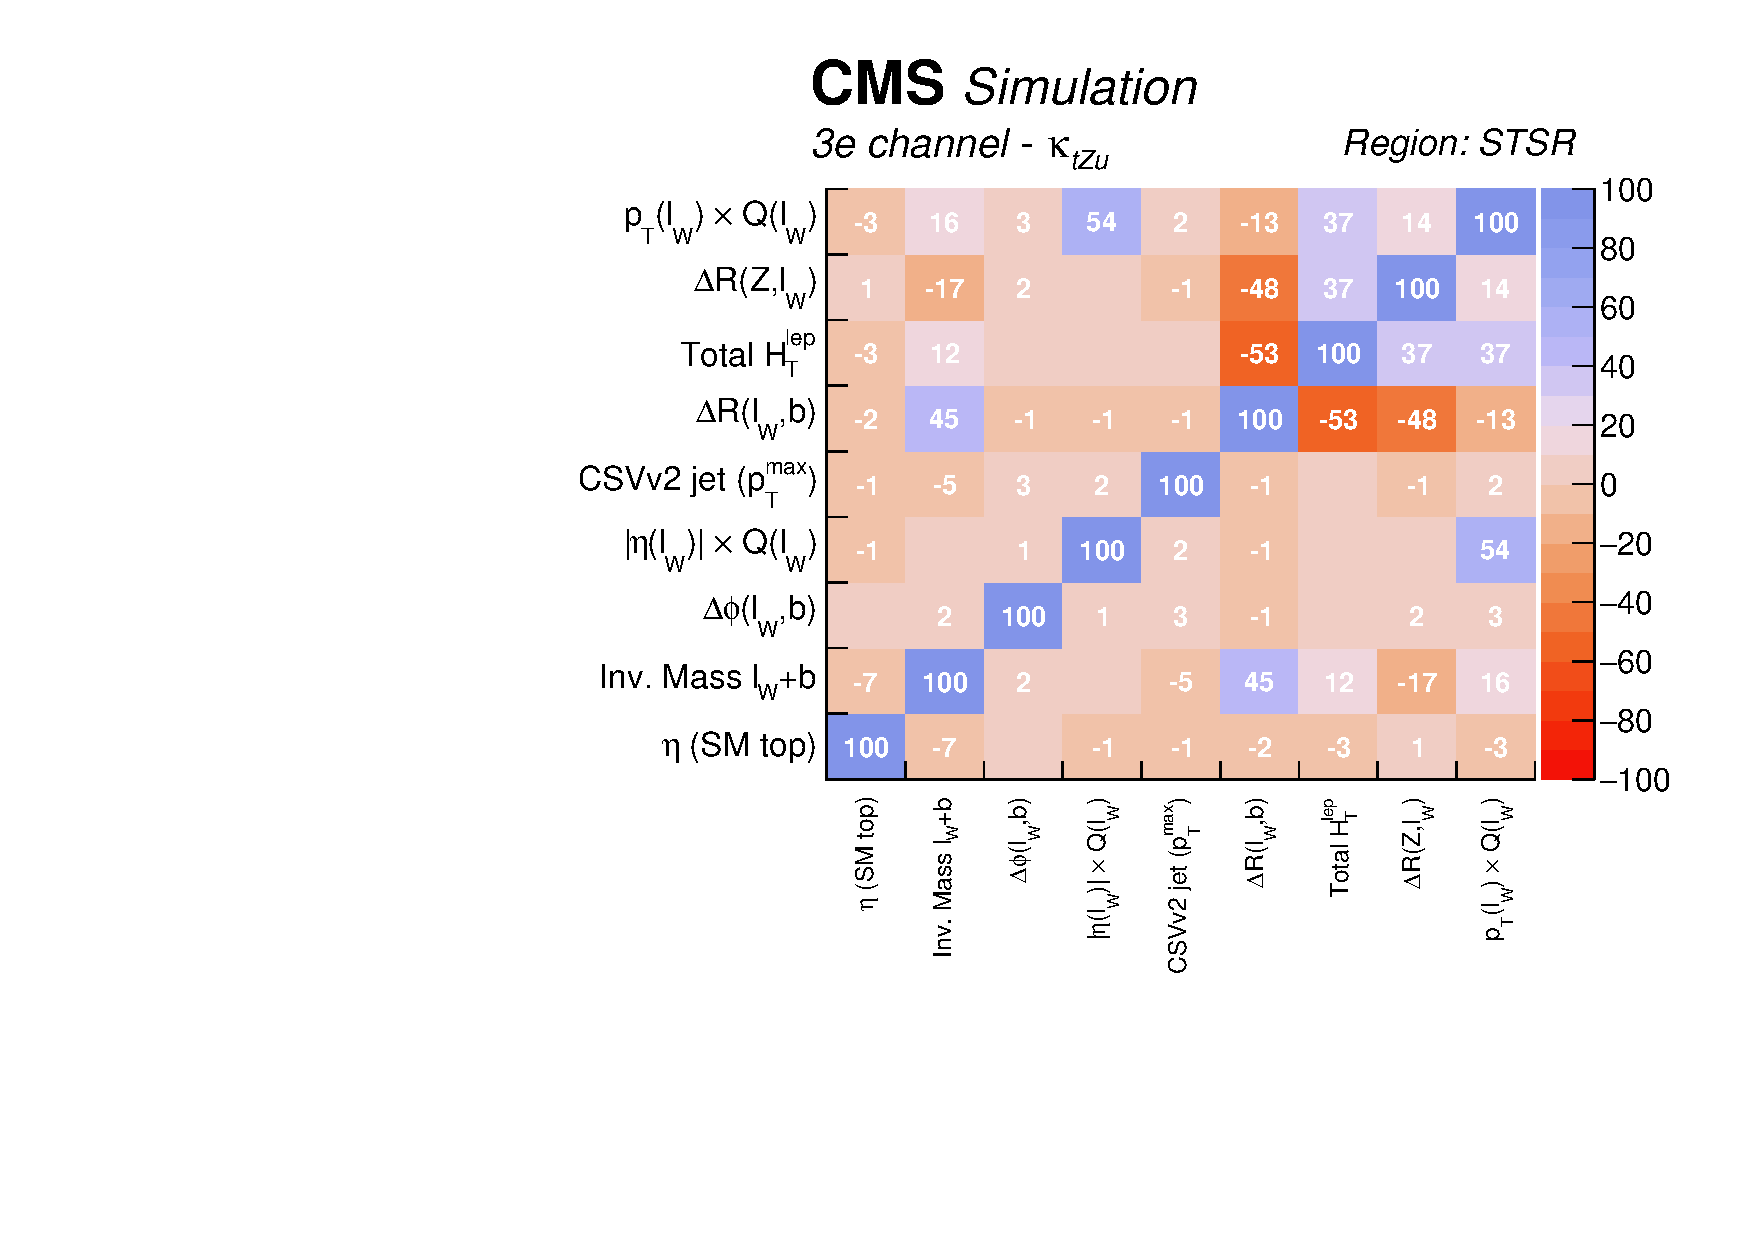
\includegraphics[width=0.49\linewidth]{6_Search/Figures/PlotsTechnics/correlationsigZutsingletopeee}
	\caption{The correlations between the input variables used to create the multivariate discriminant in the \STSR, for the \Zut\ signal. For the \mumumu\ (left,top), \emumu\ (right,top), \eemu\ (left, bottom) and \eee\ (right,bottom) three-lepton channel.}
	\label{fig:correlationsigzutsingletop}
\end{figure}

\clearpage

The resulting multivariate discriminator D is shown in \fig{fig:sigvsbkgtestzutsingletop} for all three-lepton channels. In these plots one can observe that there is a clear discrimination between the FCNC single top quark signal and the backgrounds. Furthermore, one can investigate the procedure by cross checking the distribution from the training sample with an independent testing sample. As can be seen in the distributions, these samples agree with each other. Hence there is no overtraining for the BDT method and the testing and training sample show the same separation power. 
\begin{figure}[htbp]
	\centering
	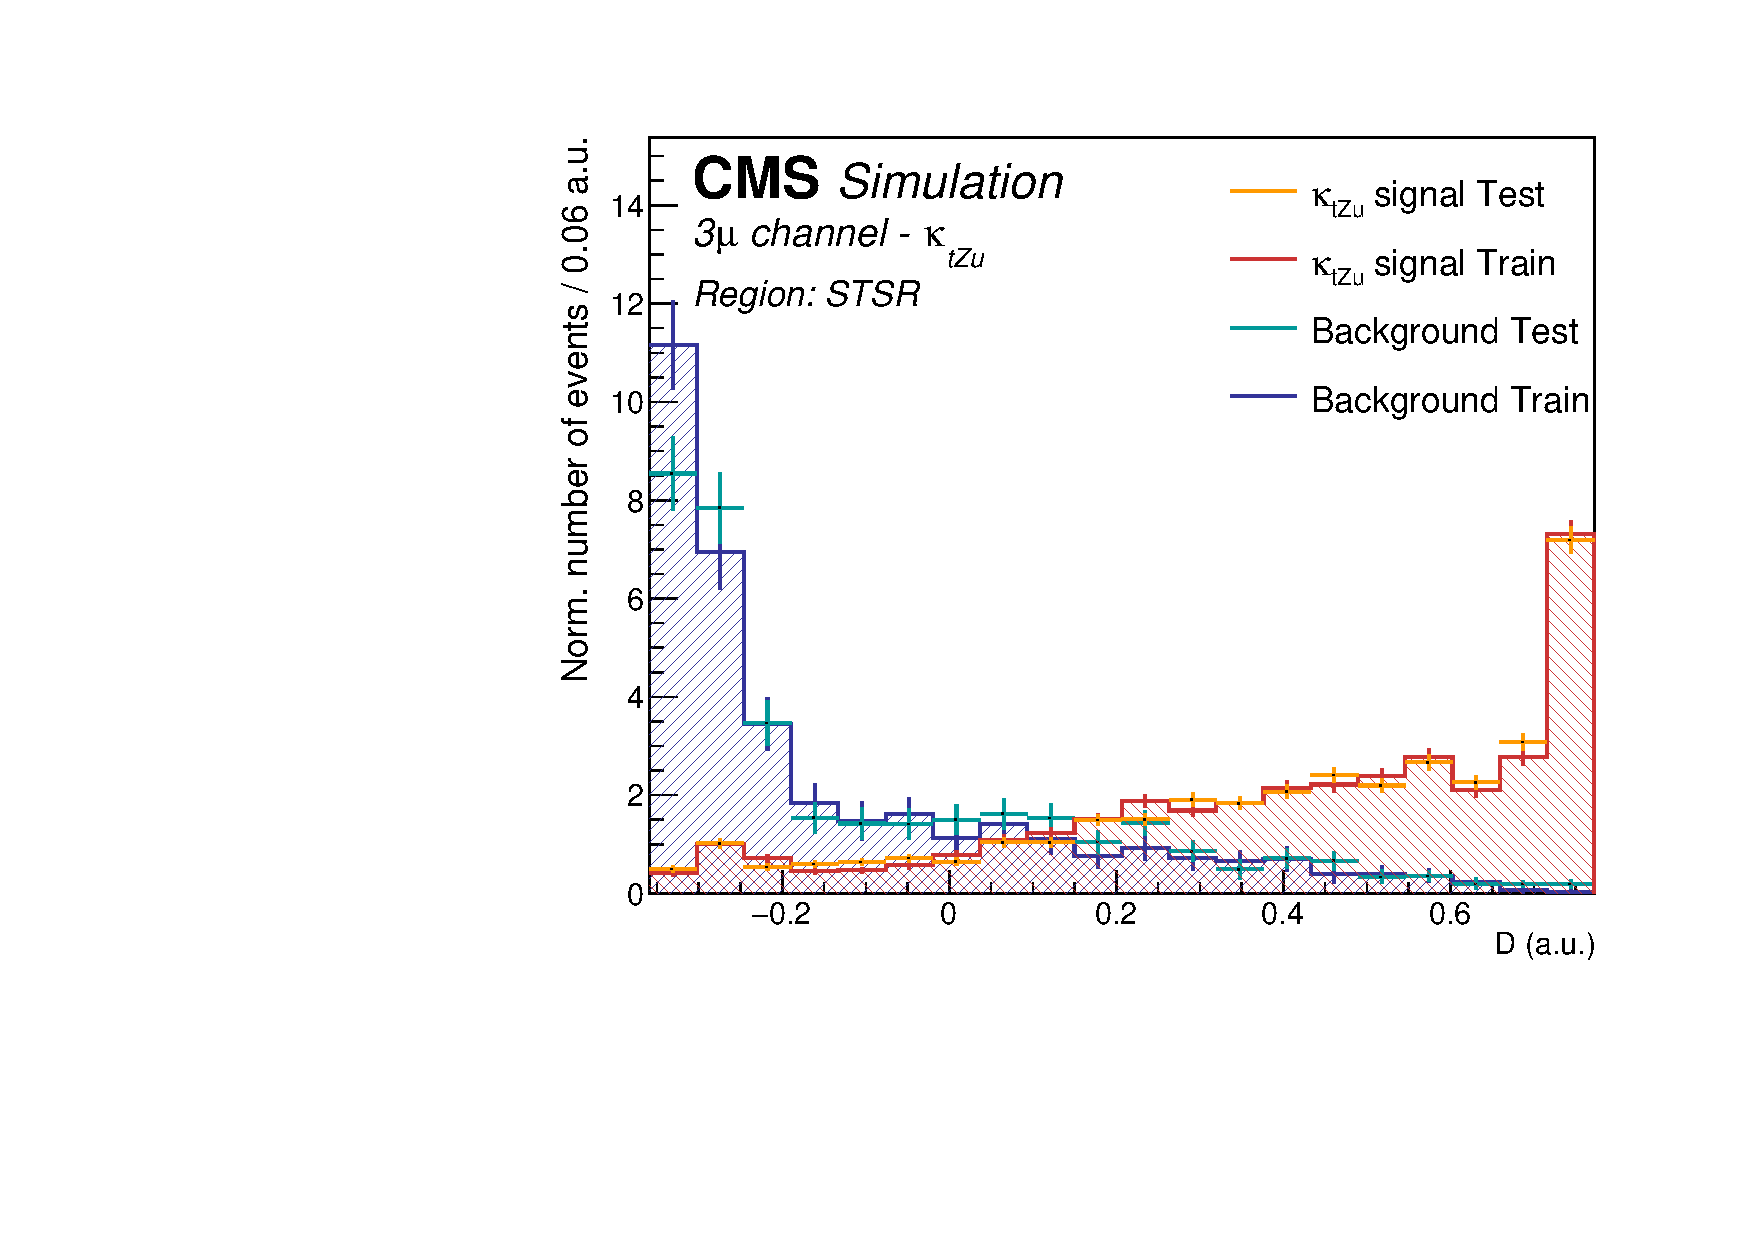
\includegraphics[width=0.49\linewidth]{6_Search/Figures/PlotsTechnics/SigVsBkgTestZutsingletopuuu}
	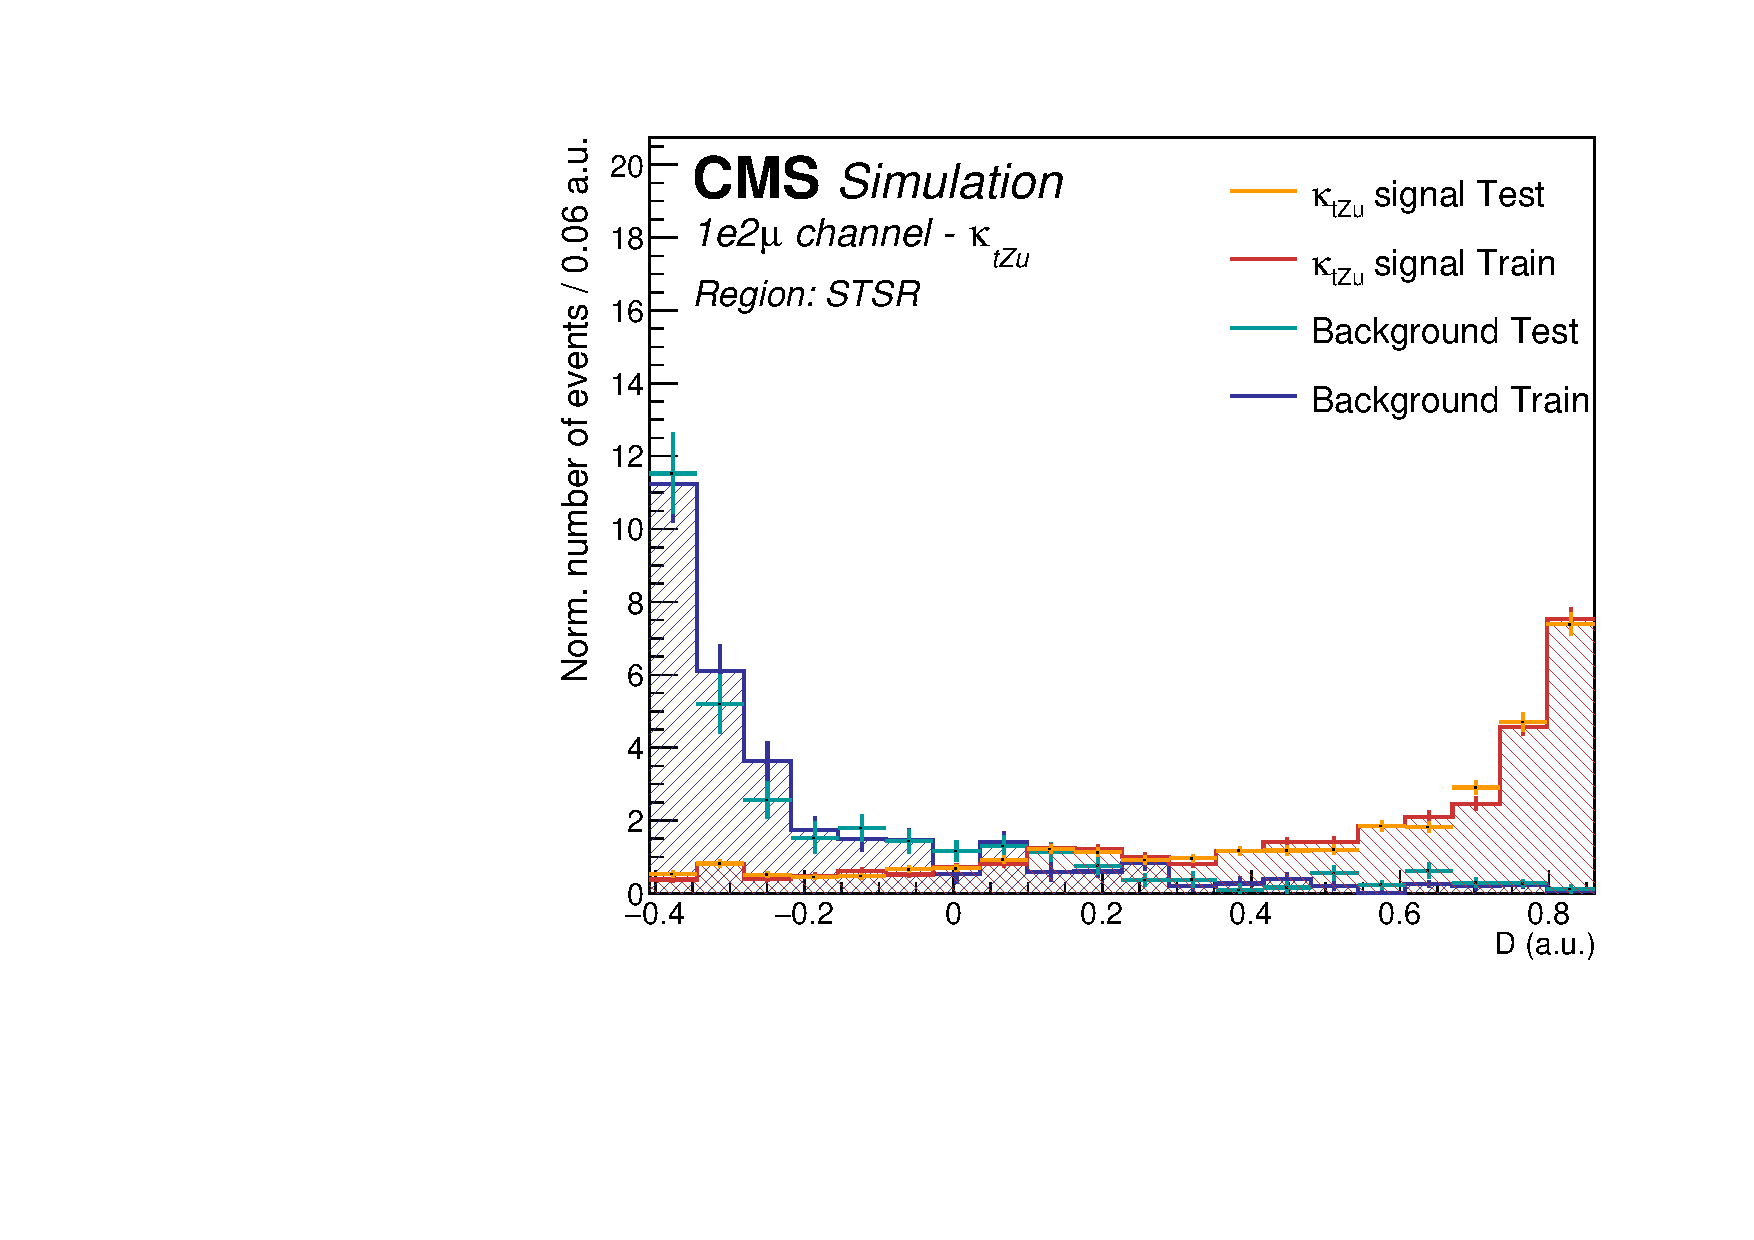
\includegraphics[width=0.49\linewidth]{6_Search/Figures/PlotsTechnics/SigVsBkgTestZutsingletopuue}
	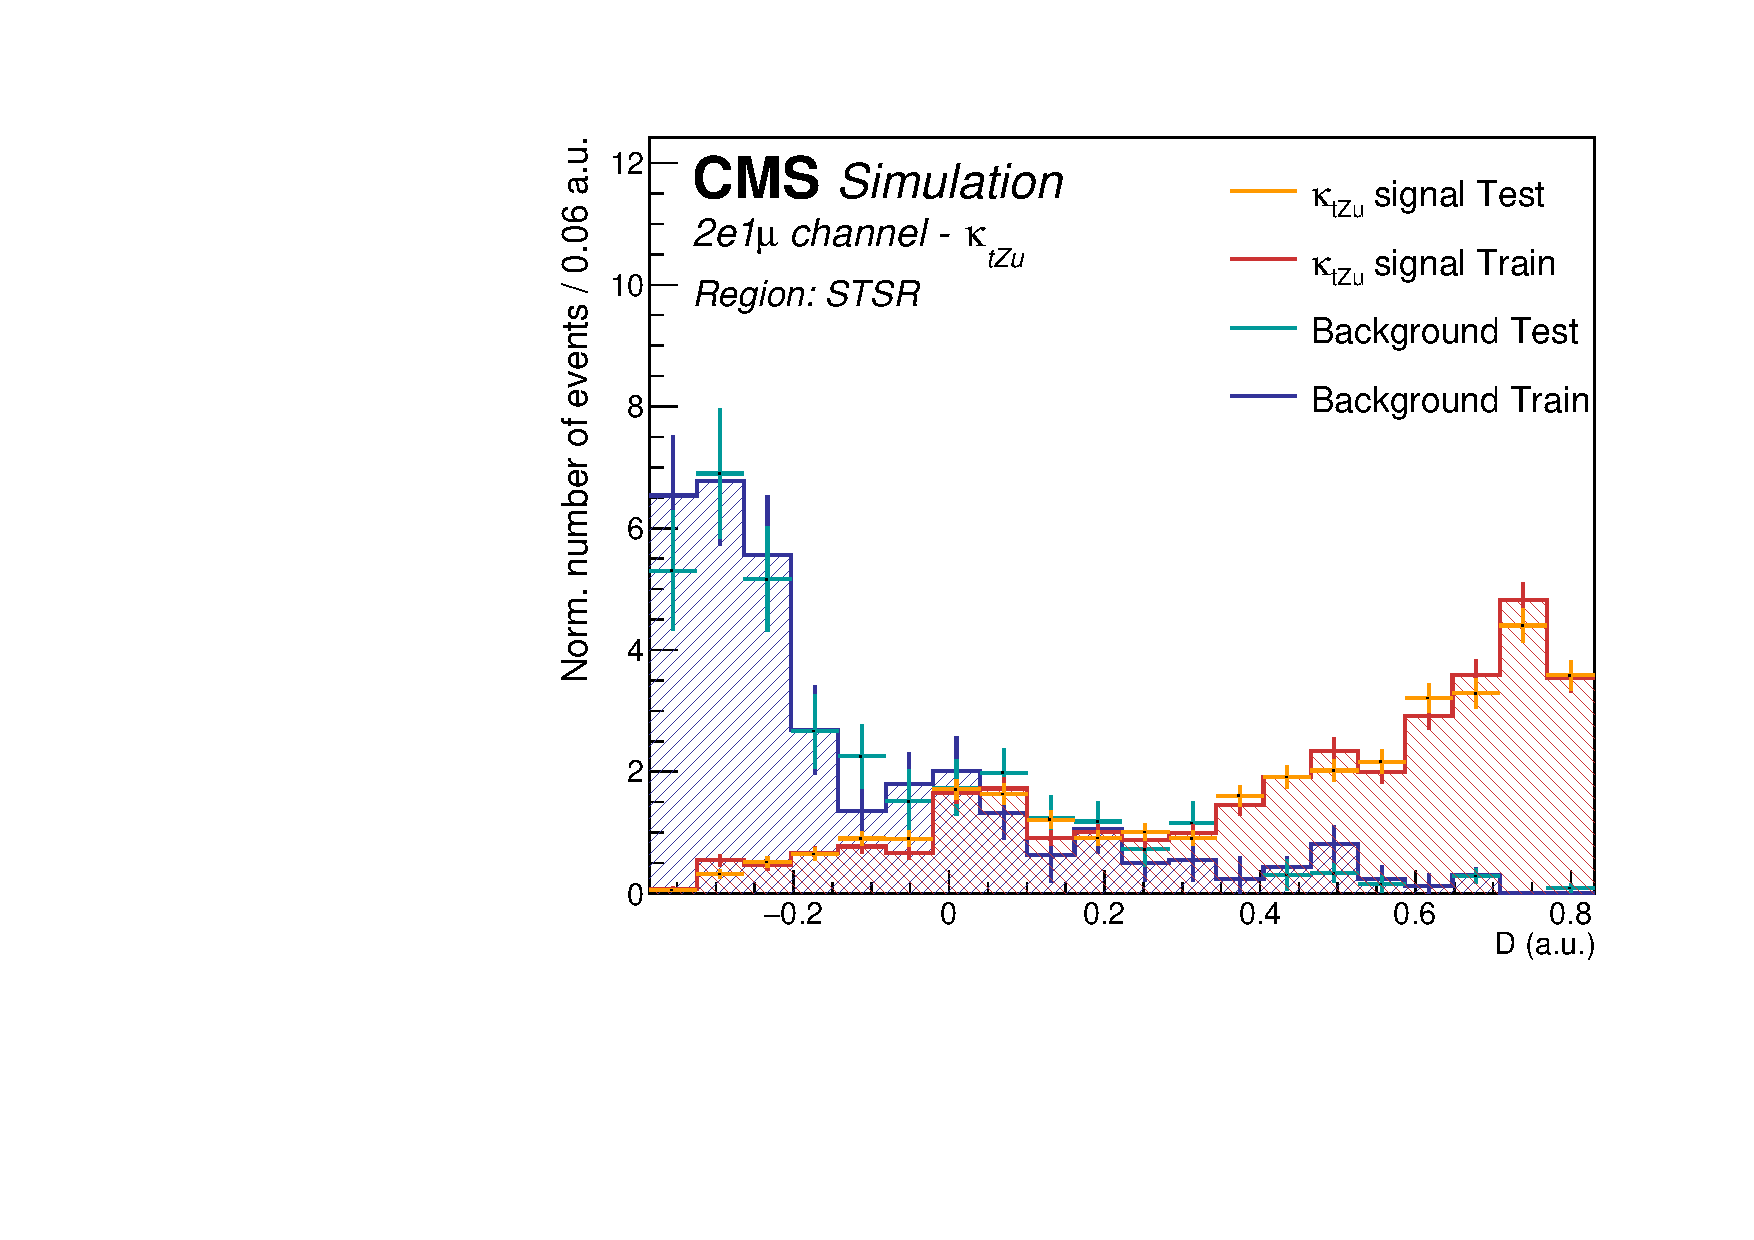
\includegraphics[width=0.49\linewidth]{6_Search/Figures/PlotsTechnics/SigVsBkgTestZutsingletopeeu}
	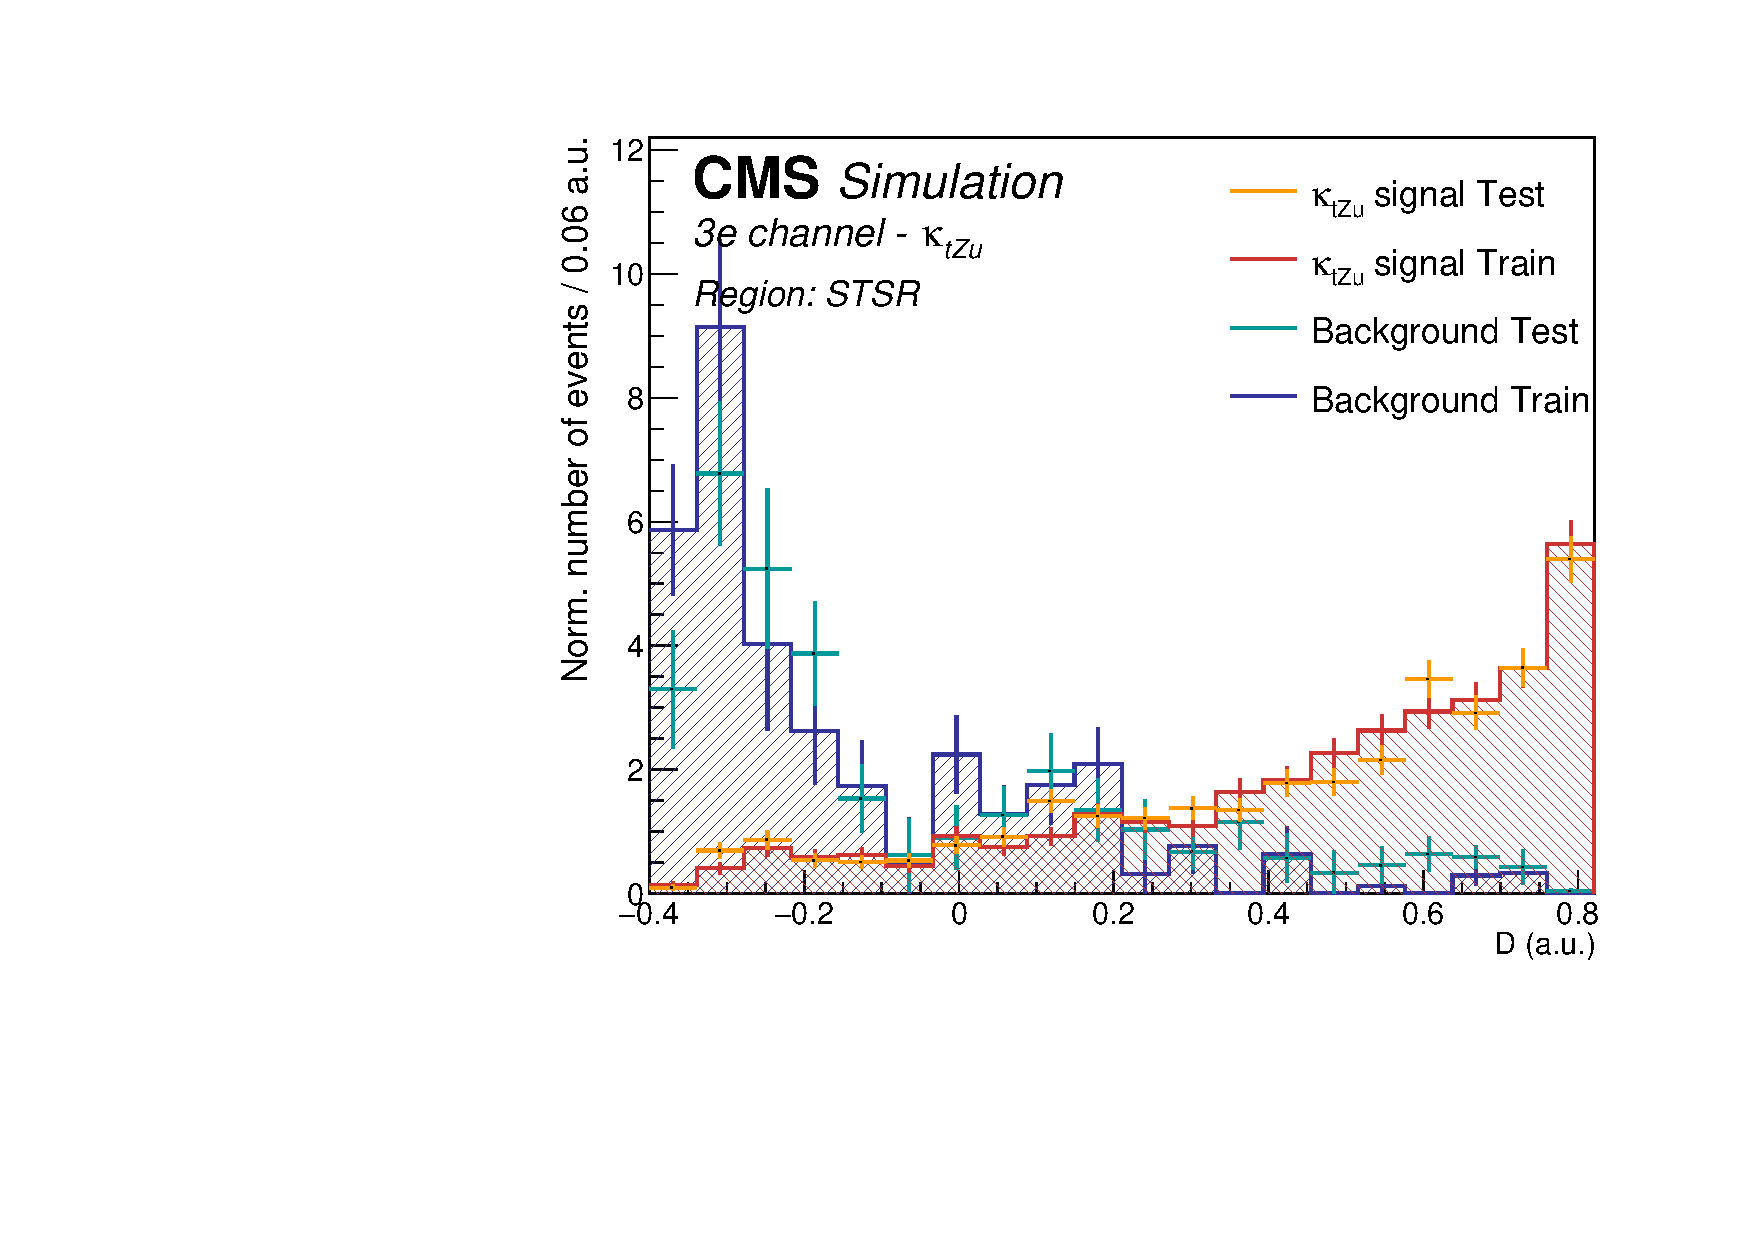
\includegraphics[width=0.49\linewidth]{6_Search/Figures/PlotsTechnics/SigVsBkgTestZutsingletopeee}
\caption{The normalised distributions of the resulting  multivariate discriminators D in the \STSR, for the \Zut\ signal. For the \mumumu\ (left,top), \emumu\ (right,top), \eemu\ (left, bottom) and \eee\ (right,bottom) three-lepton channel.}
	\label{fig:sigvsbkgtestzutsingletop}
\end{figure}

Additionally, the Receiving Operator Characteristic (ROC) curves for the testing and training samples are shown in \fig{fig:roczutsingletop}. One can observe that for all channels there is a clear separating power and that the ROC curve of the testing sample is a bit below the one for the training sample, resulting in slightly worse performance when testing the method. This is the most present in the \eee\ channel, where there is a lack of statistics. However, the distinction between signal and background like is clearly still there.
\begin{figure}[htbp]
	\centering
	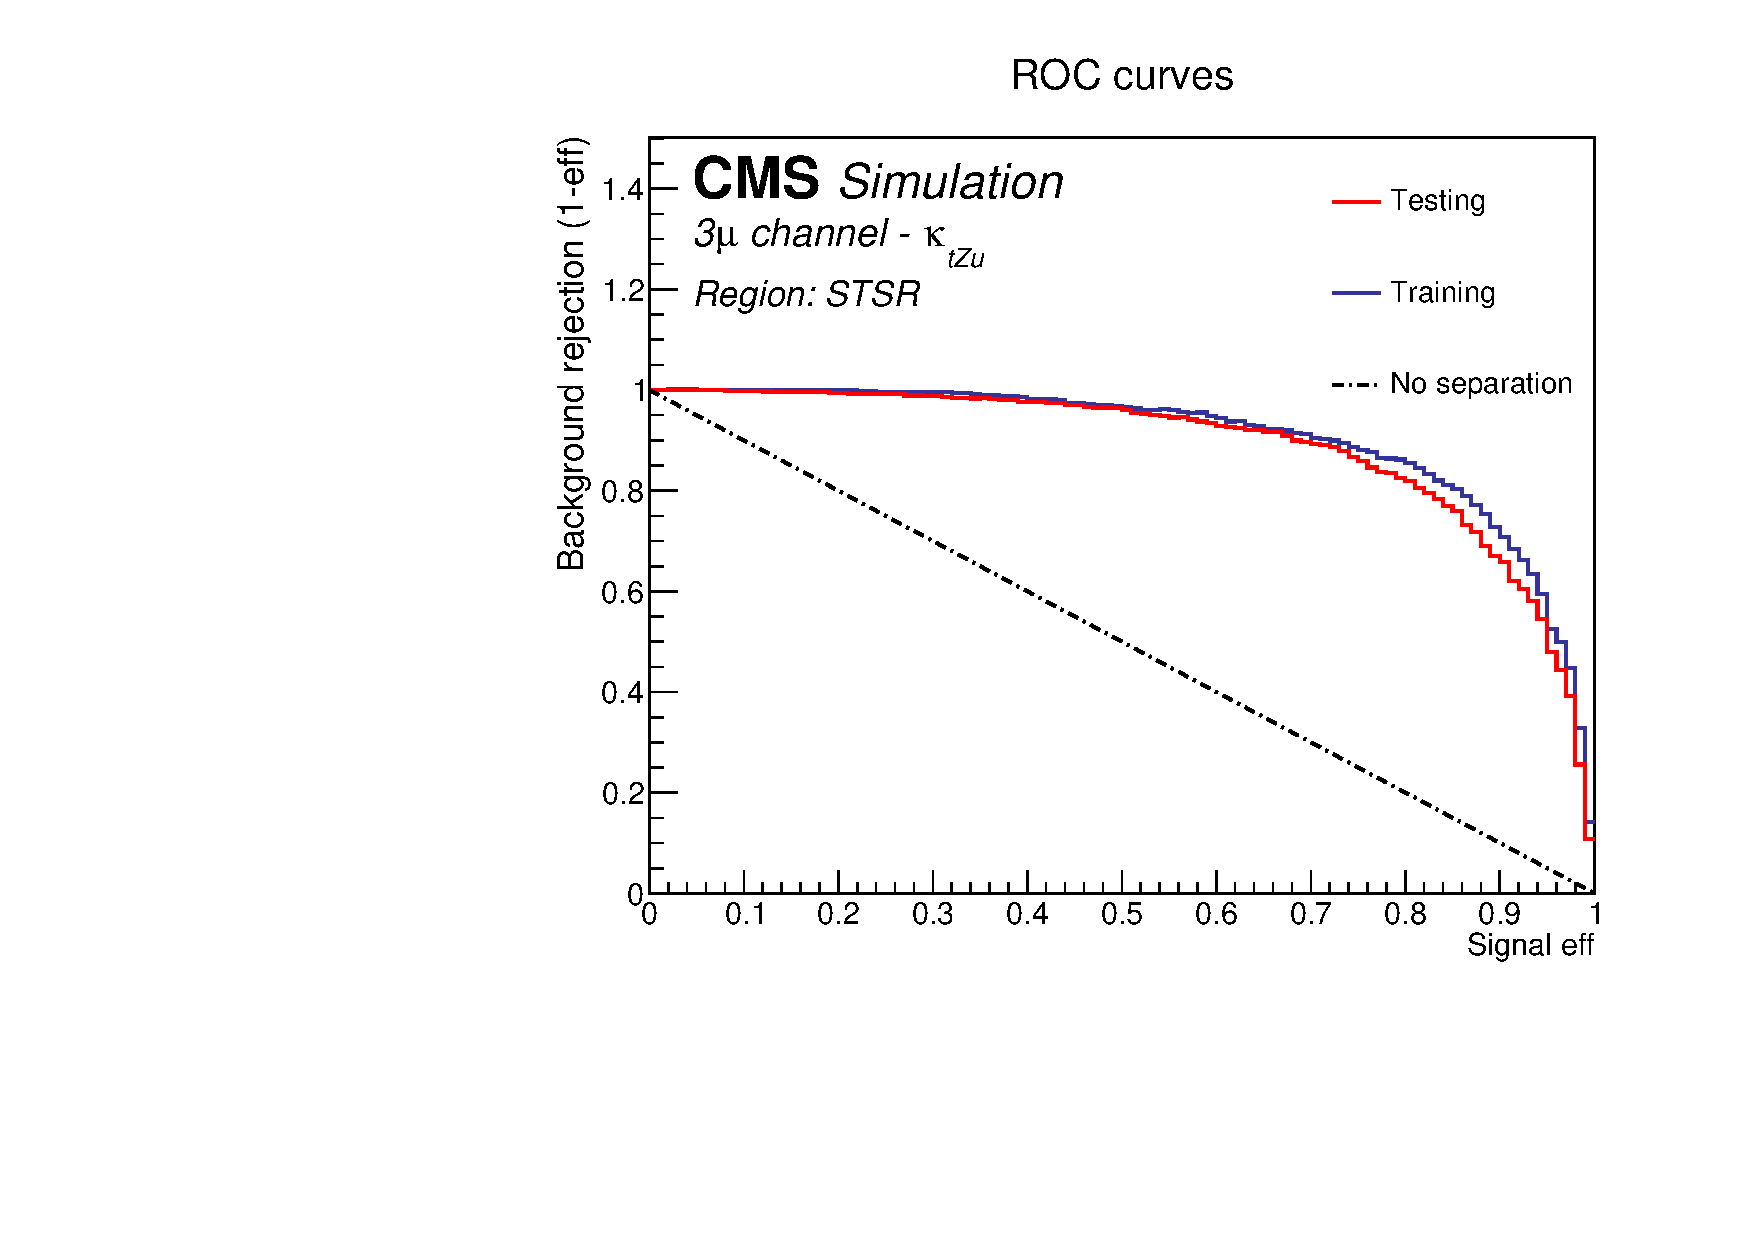
\includegraphics[width=0.49\linewidth]{6_Search/Figures/PlotsTechnics/ROCZutsingletopuuu}
	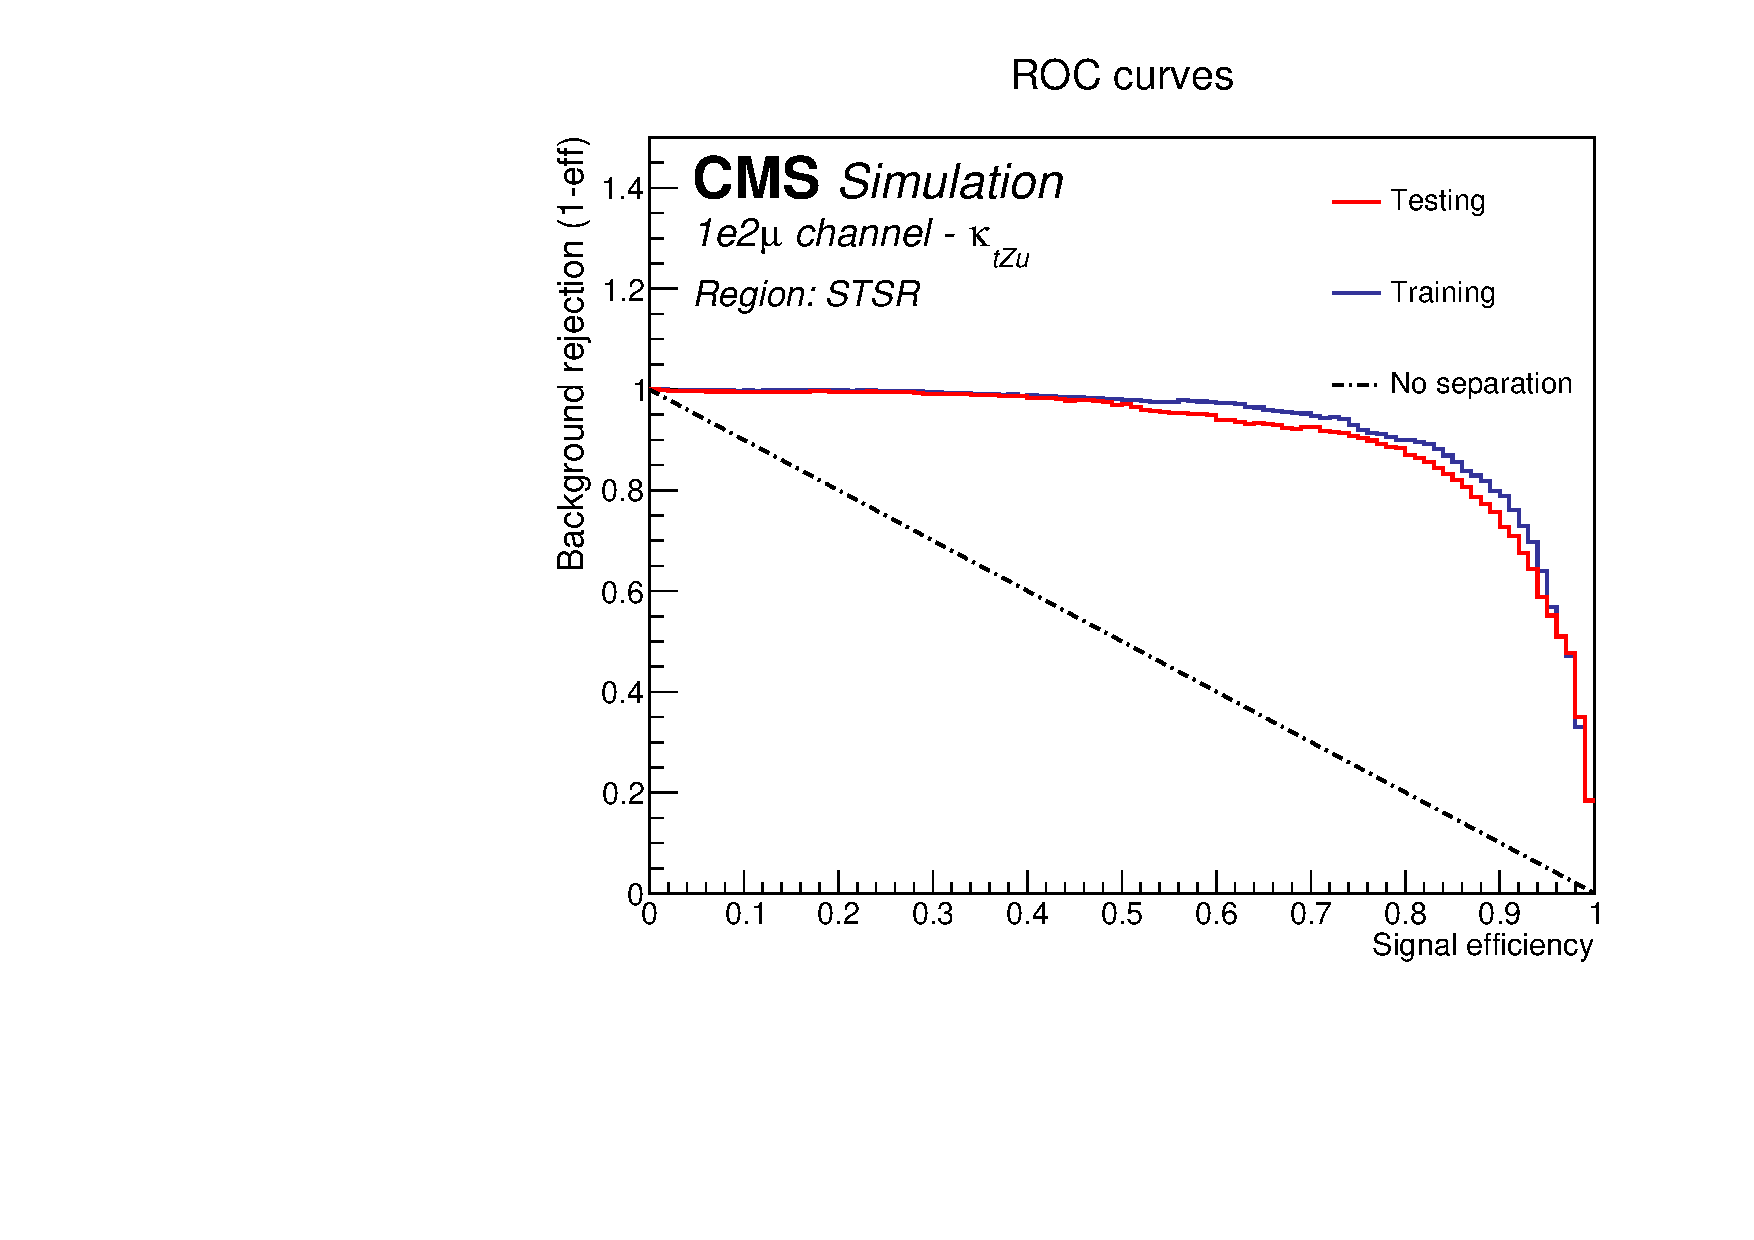
\includegraphics[width=0.49\linewidth]{6_Search/Figures/PlotsTechnics/ROCZutsingletopuue}
	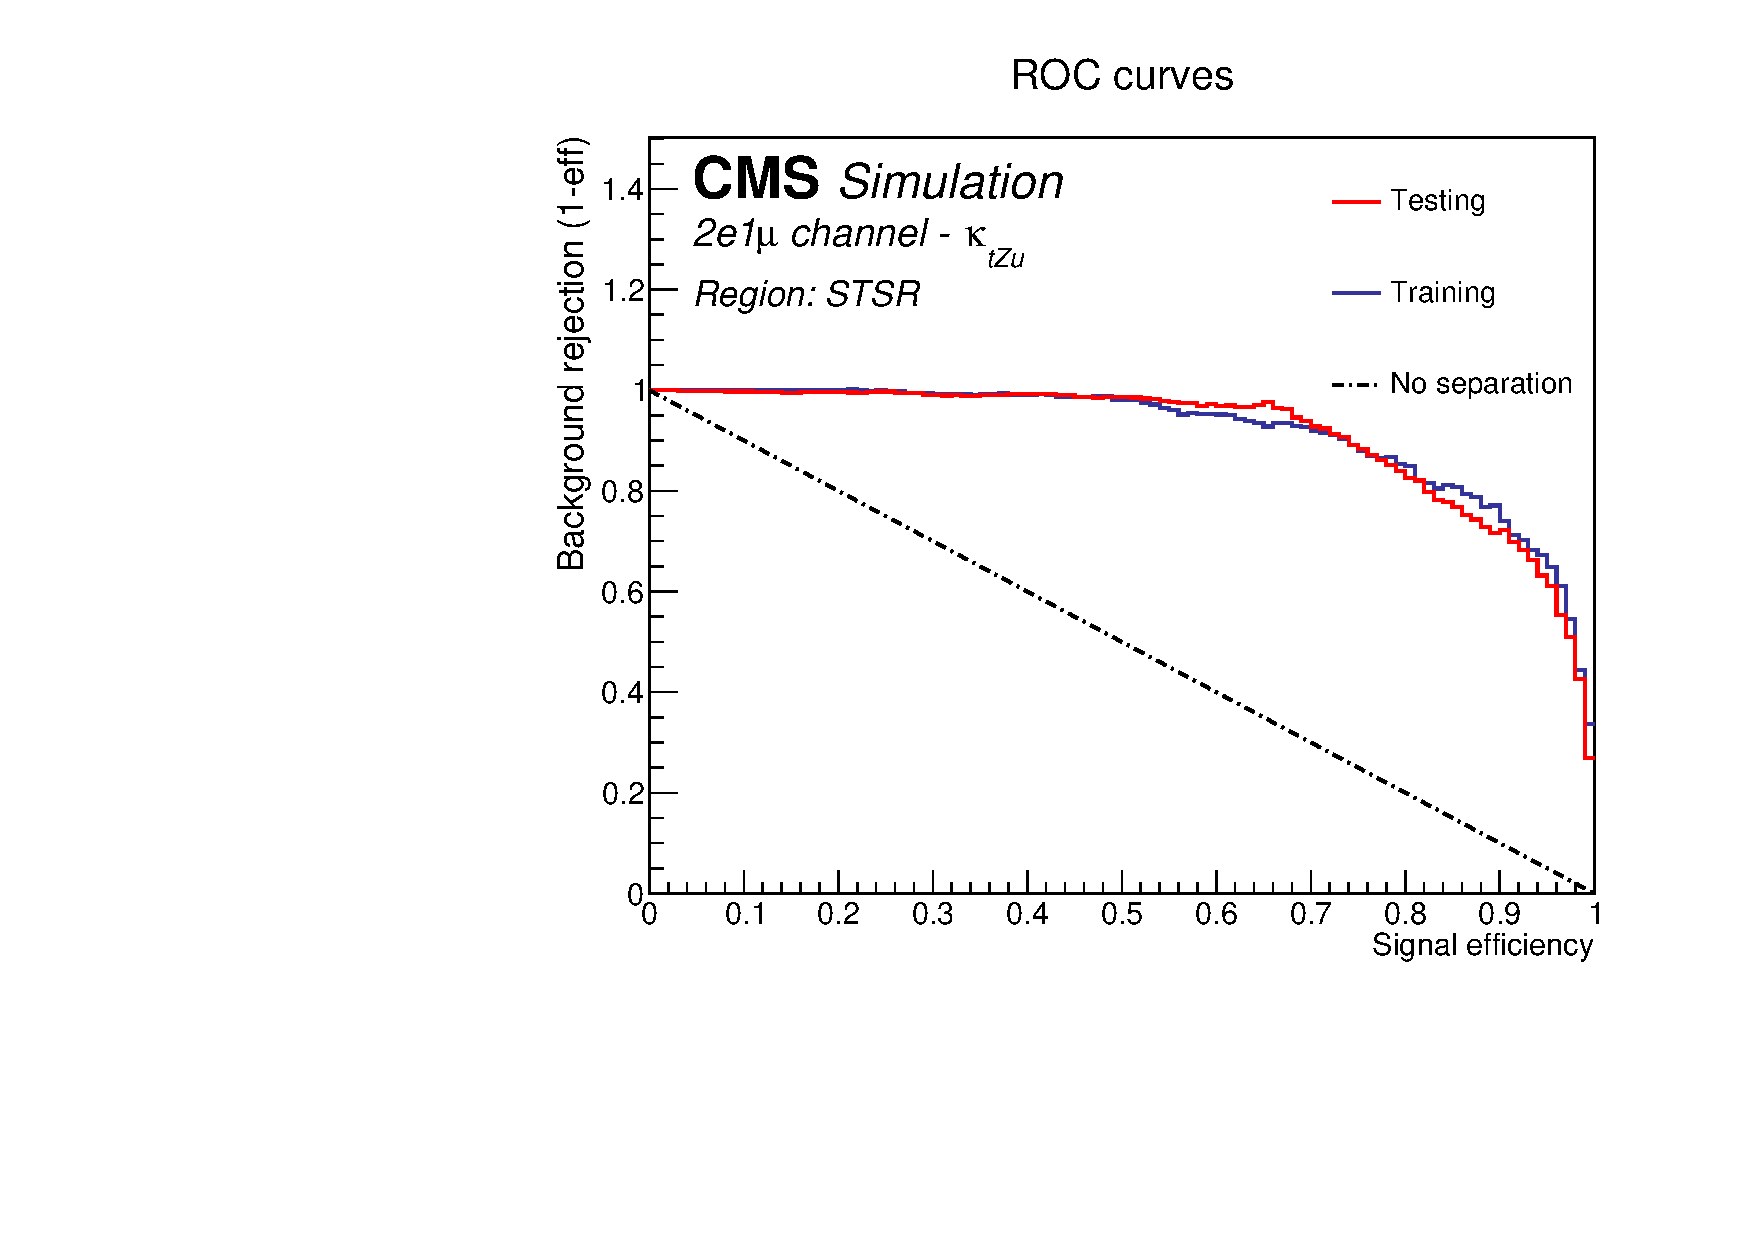
\includegraphics[width=0.49\linewidth]{6_Search/Figures/PlotsTechnics/ROCZutsingletopeeu}
	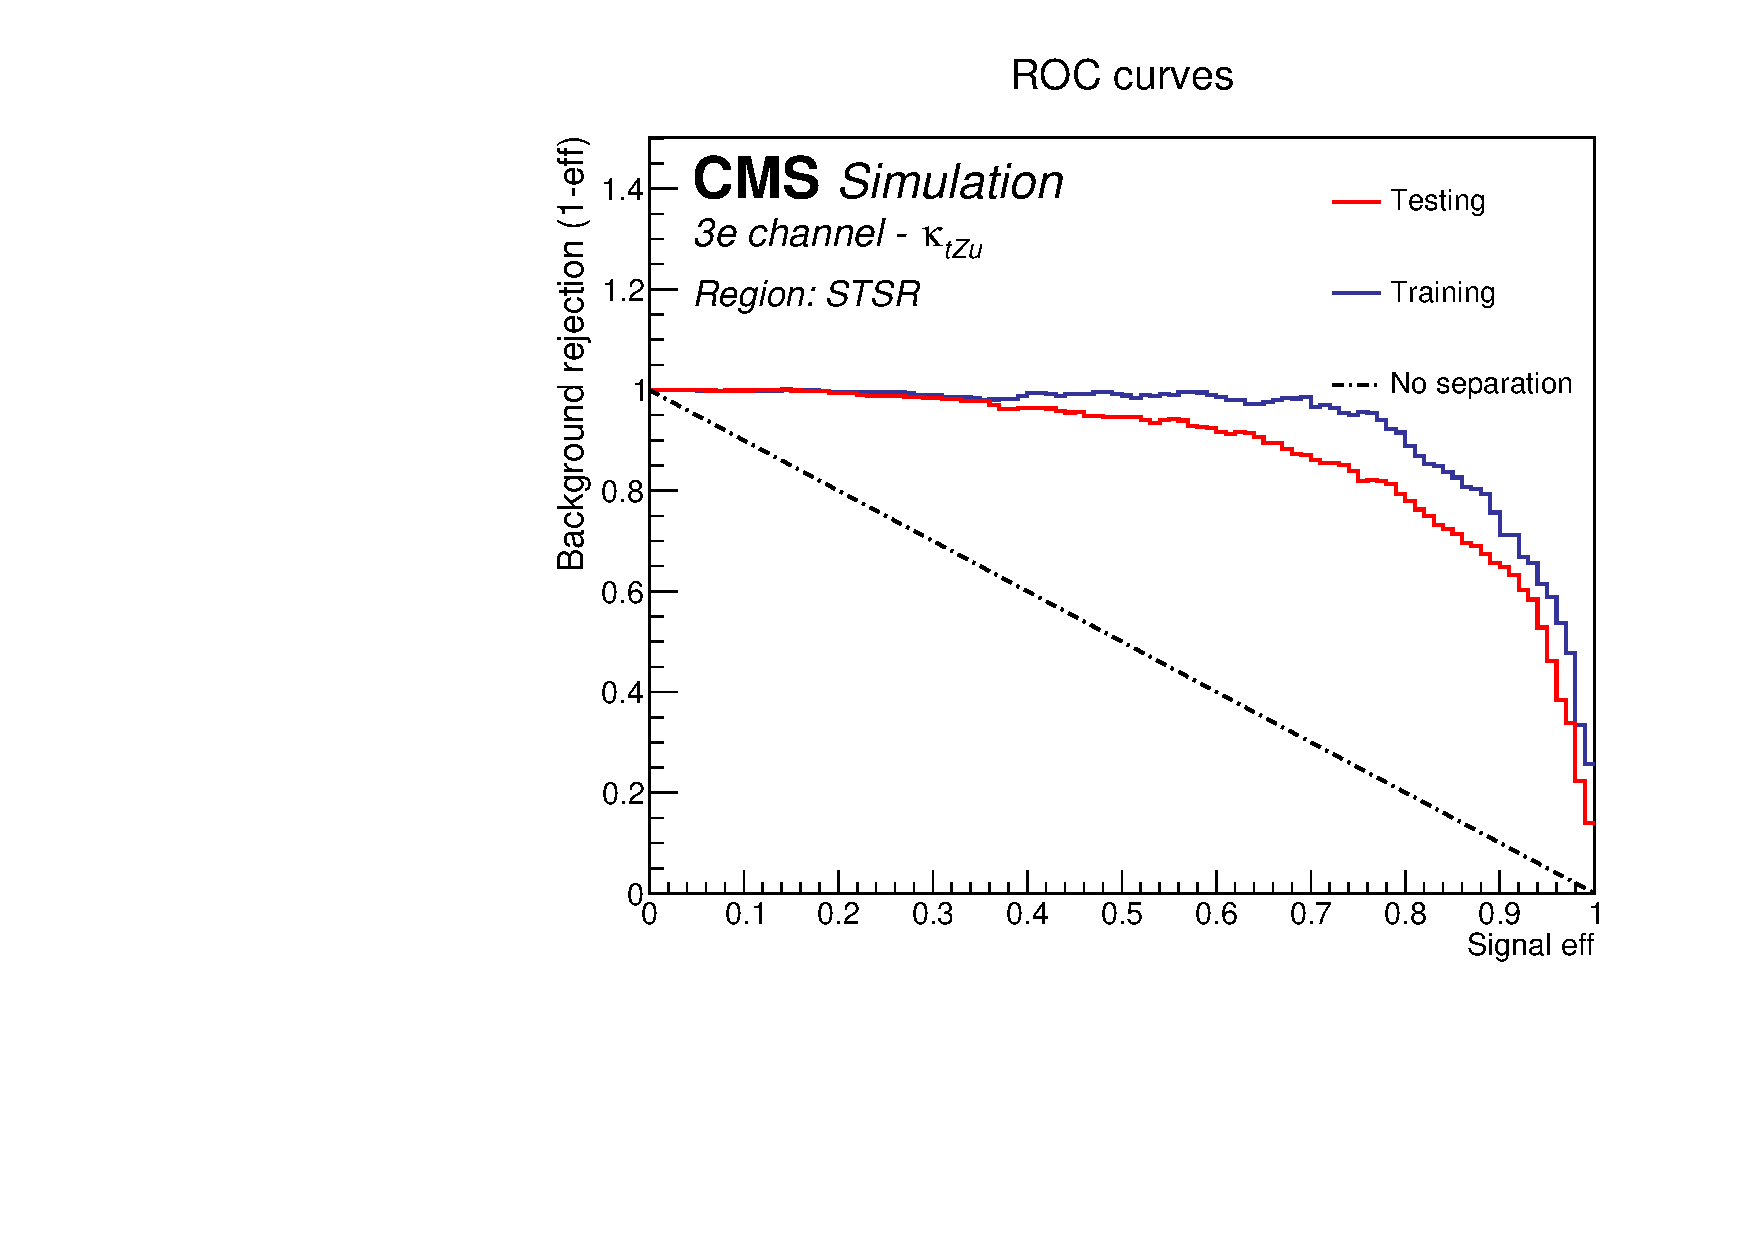
\includegraphics[width=0.49\linewidth]{6_Search/Figures/PlotsTechnics/ROCZutsingletopeee}
	\caption{ROC curves of the resulting  multivariate discriminators D in the \STSR, for the \Zut\ signal. For the \mumumu\ (left,top), \emumu\ (right,top), \eemu\ (left, bottom) and \eee\ (right,bottom) three-lepton channel. The dashed line represents the case of no separation power.}
	\label{fig:roczutsingletop}
\end{figure}




\clearpage
\subsection{BDT training in the \TTSR\ for the \Zut\ interaction}
\label{sec:BDTTTSRZUT}
In this region, the BDT is trained to enhance the top quark pair and the single top FCNC signals at the same time. The contribution of the \NPL\ background is again not considered during training. The top quark pair FCNC signal has the largest contribution in this region. The top quark pair FCNC signal expects one \Pbottom\ jet (SM b~jet), one lepton (\PW\ lepton ) and missing transverse energy coming from the \SM\ top quark decay (SM top quark). The other top quark decays through the FCNC vertex and creates two leptons from the \PZ\ boson decay and a light quakr (up or charm). 

In this region, the main backgrounds are the \ttZ, \SM\ \tZq, and \WZ+jets processes. Again, the events originating from the \WZ+jet process, are entering the \STSR\ due to a b~jet produced by gluon splitting or the light-flavour jets that are mis-tagged as b~jets.  The SM \tZq\ has exactly the same signature as the top quark pair FCNC signal.  The \ttZ\ process is entering the analysis when both tops are decaying leptonically and on b jet is missing from the reconstruction or in association with not prompt-leptons. 


  In \fig{fig:toppairZutnormalized}, the input variables used to create the multivariate discriminant are shown for the \mumumu\ channel. The distributions for the other three-lepton channels are given in \App{app:BDTcorrZutTop}. For the \ttZ\ process, a \PZ\ boson is radiated of one of the top quarks of a top quark pair production process. Hence, no top quark is expected to be reconstructed from a light-flavour jet and \PZ\ boson. For the \SM\ \tZq\ process this also the case. Therefore, the invariant mass of the reconstructed FCNC top quark, as well as the distances in the $\phi\eta$-plane between the \PZ\ boson and the FCNC light-flavour jet are used as discriminating variables for this search. For background, the distribution invariant mass of the FCNC top quark has a broader peak than the FCNC signal which is peaking at the known top quark mass. The distribution of the distance between the FCNC jet and the reconstructed \PZ\ boson is peaking at higher values for the backgrounds compared to signal. Also the invariant mass of the \PZ\ boson is used as discriminating variable since the distribution the peak is finer for the FCNC signal compared to the background. 
  

   For the same reasons as in the previous sections, the pseudorapidity of the SM top quark,  the invariant mass of the \PW\ lepton and the \SM\ b jet, as well as their distances in the $\phi\eta$-plane are considered. For the backgrounds, the invariant mass of the \PW\ lepton and \SM\ jet system has a longer tail. Furthermore, the difference in distance  between the \PW\ lepton and \SM\ b jet peaks at lower values for the FCNC signal. The distribution of the difference in the azimuthal angle peaks at $\pm1$ for signal, while at $\pm 3$ for the background processes. Furthermore, the distribution of the minimal distance in the $\phi\eta$-plane between the \PW\ lepton and all the jets in the event is peaking at lower values for the FCNC signal than for backgrounds. This is due to the fact that for the FCNC signal events this distance will be most likely the distance from the SM b  jet, while for the \ttZ\ and \tZq\ processes this could be biased due to radiation, and for \WZ+jets events this distance will come from an FSR jet.  Also the number of b-tagged jets according to the CSVv2 medium working point is used in creating the multivariate discriminator. For FCNC signal this distributions peaks at one, while for background, this peaks at zero.
   
   
   For the FCNC signal, one expects that the decay products coming from the FCNC interaction in the event is opposite in direction compared the decay products of the \SM\ interaction. This is exploited by looking at the distribution of difference in azimuthal angle between the  \PZ\ boson and  \PW\ lepton. For the FCNC signal, this distribution peaks at $\pm 3$, while remaining flat for the backgrounds. Furthermore the difference in the $\phi\eta$-plane between the \SM\ b jet and FCNC jet is used as discriminating variable. For the FCNC signal, this distribution peaks around three, and is broader for the backgrounds.  The most important input variables for this region, for the \Zut\ interaction, are the invariant mass of the \PW\ lepton and the \SM\ b jet system, as well as their distance. On the third place is the number of jets tagged as being a b jet according to the CSVv2 algorithm at its medium working point. 
\begin{figure}[htbp]
	\centering
	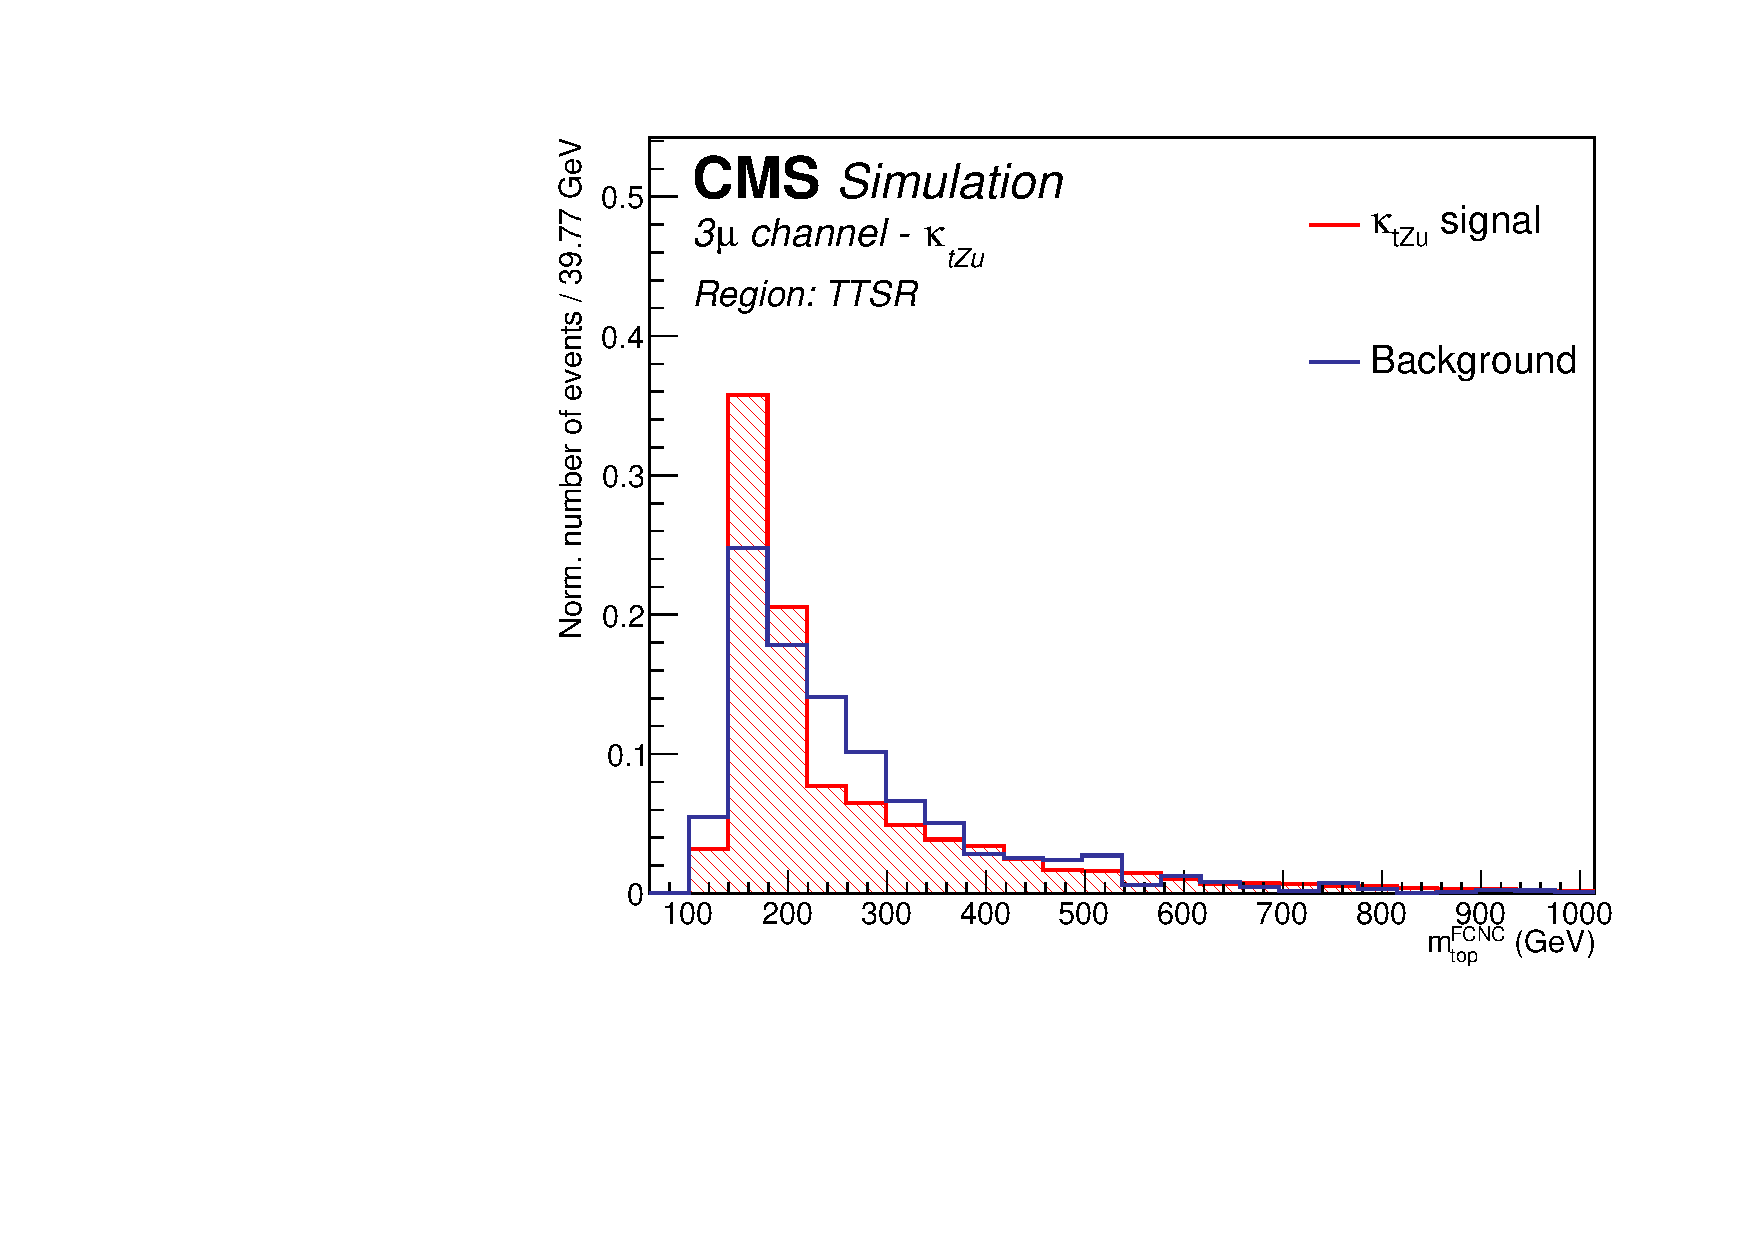
\includegraphics[width=0.3\linewidth]{6_Search/Figures/PlotsTechnics/FCNCtop_MZuttoppairuuu_norm}
	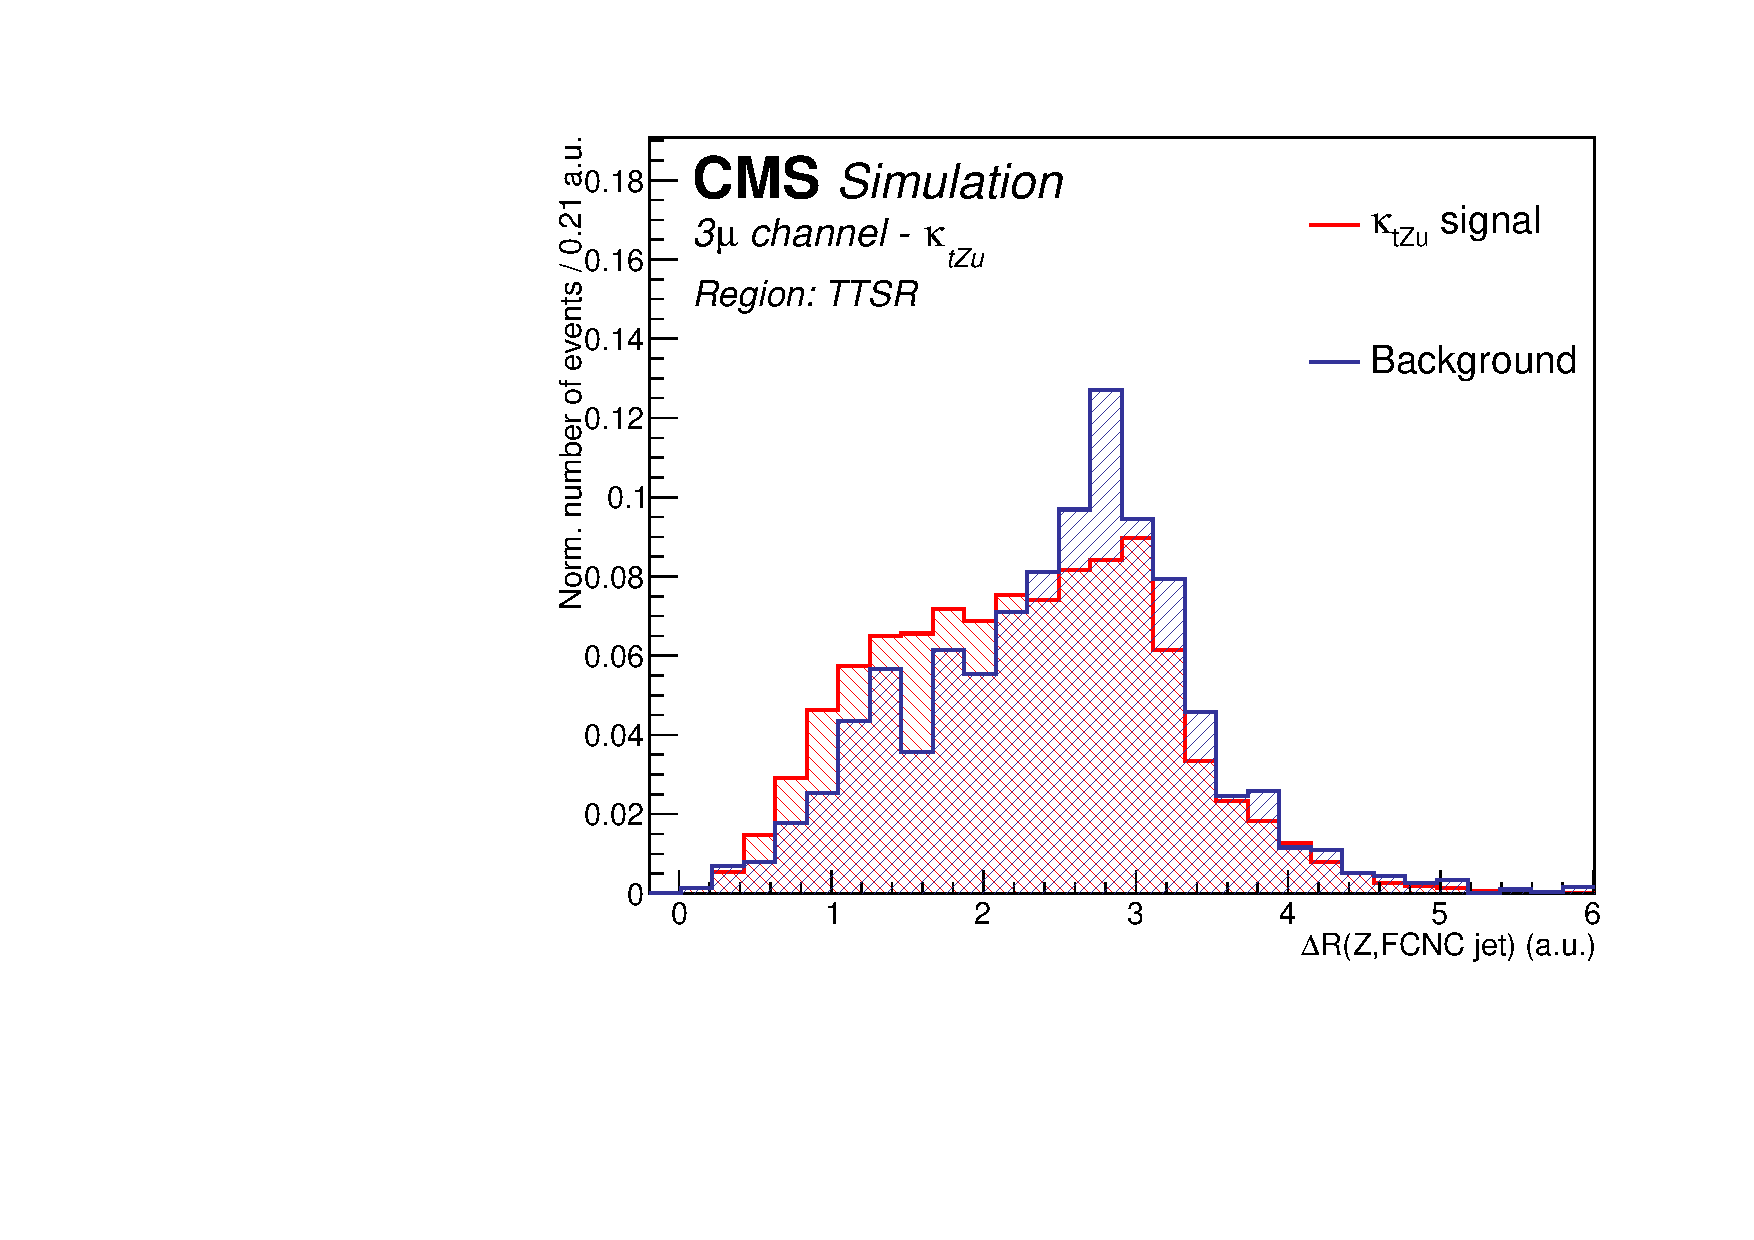
\includegraphics[width=0.3\linewidth]{6_Search/Figures/PlotsTechnics/dRZcZuttoppairuuu_norm}
	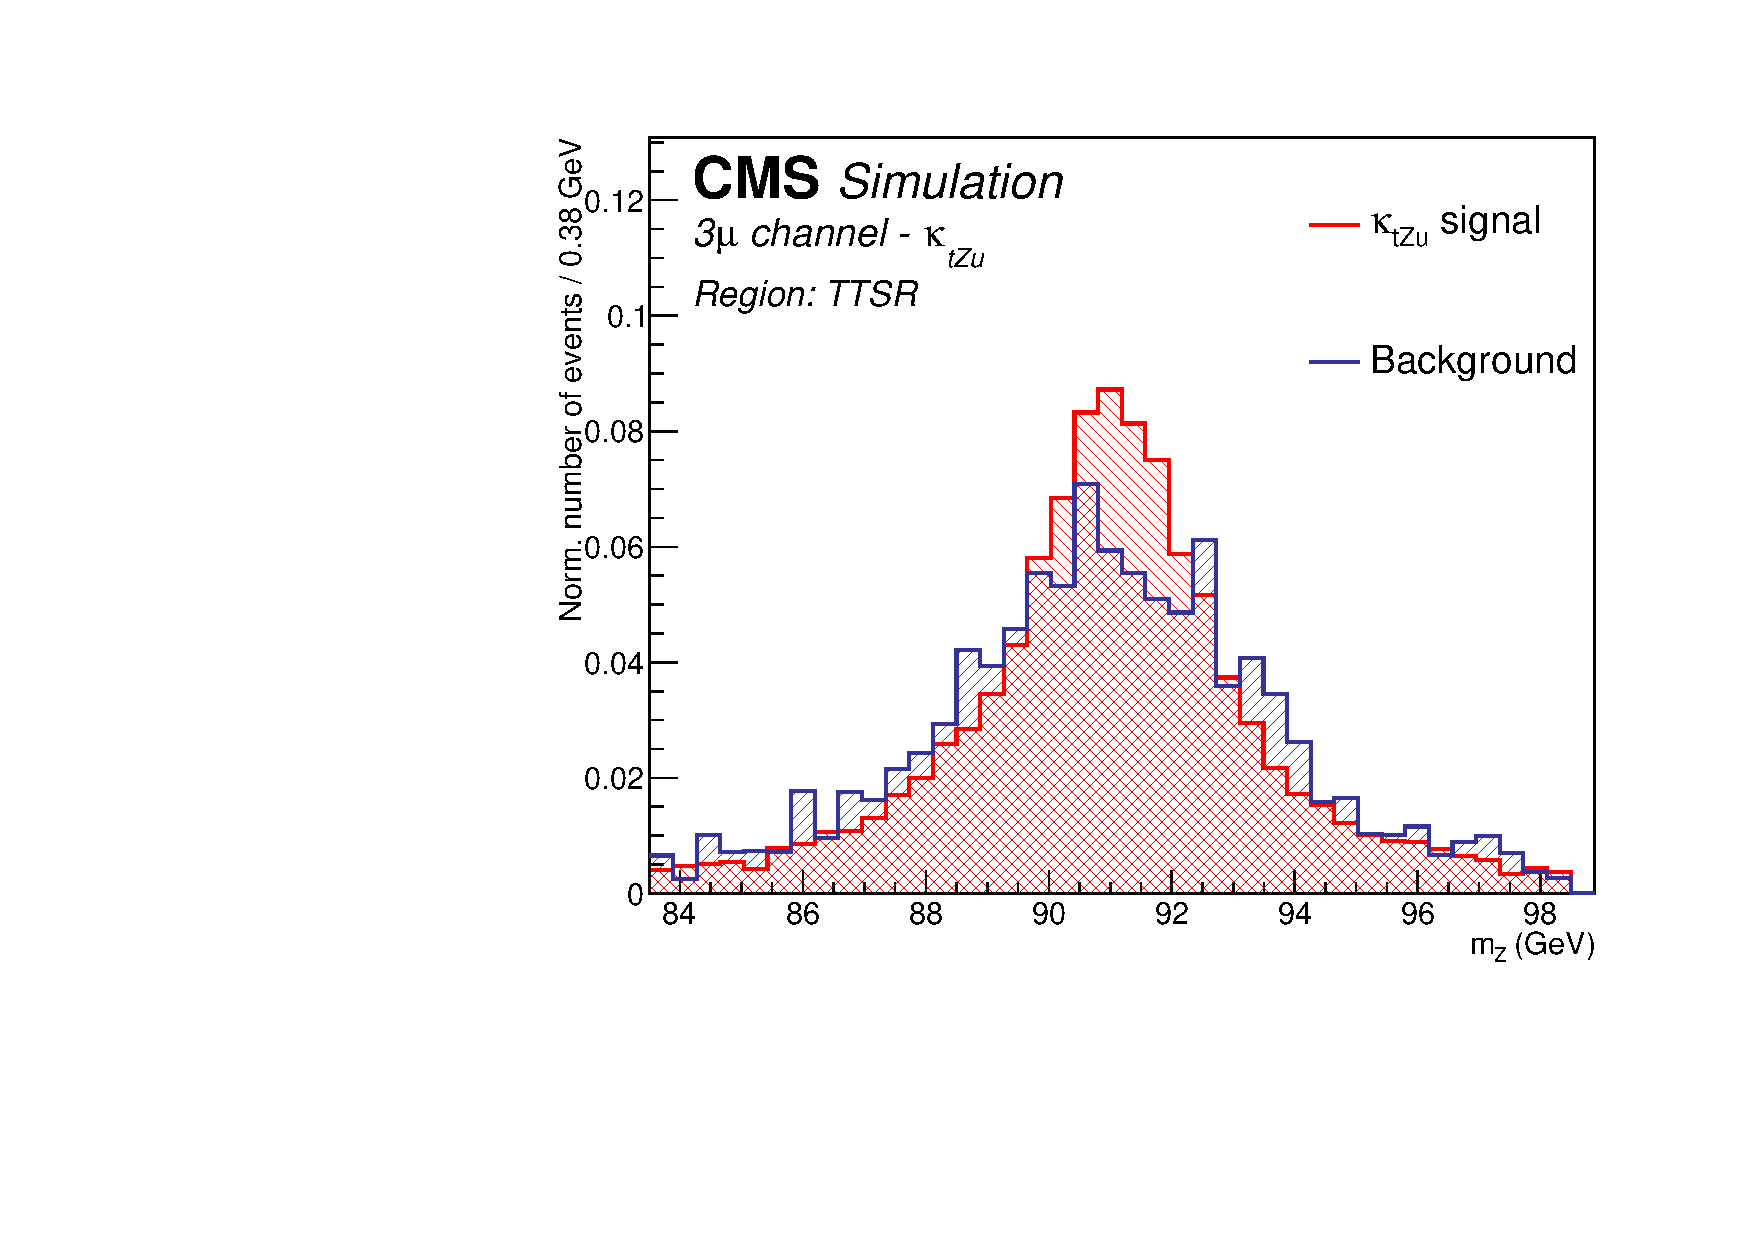
\includegraphics[width=0.3\linewidth]{6_Search/Figures/PlotsTechnics/Zboson_MZuttoppairuuu_norm}
	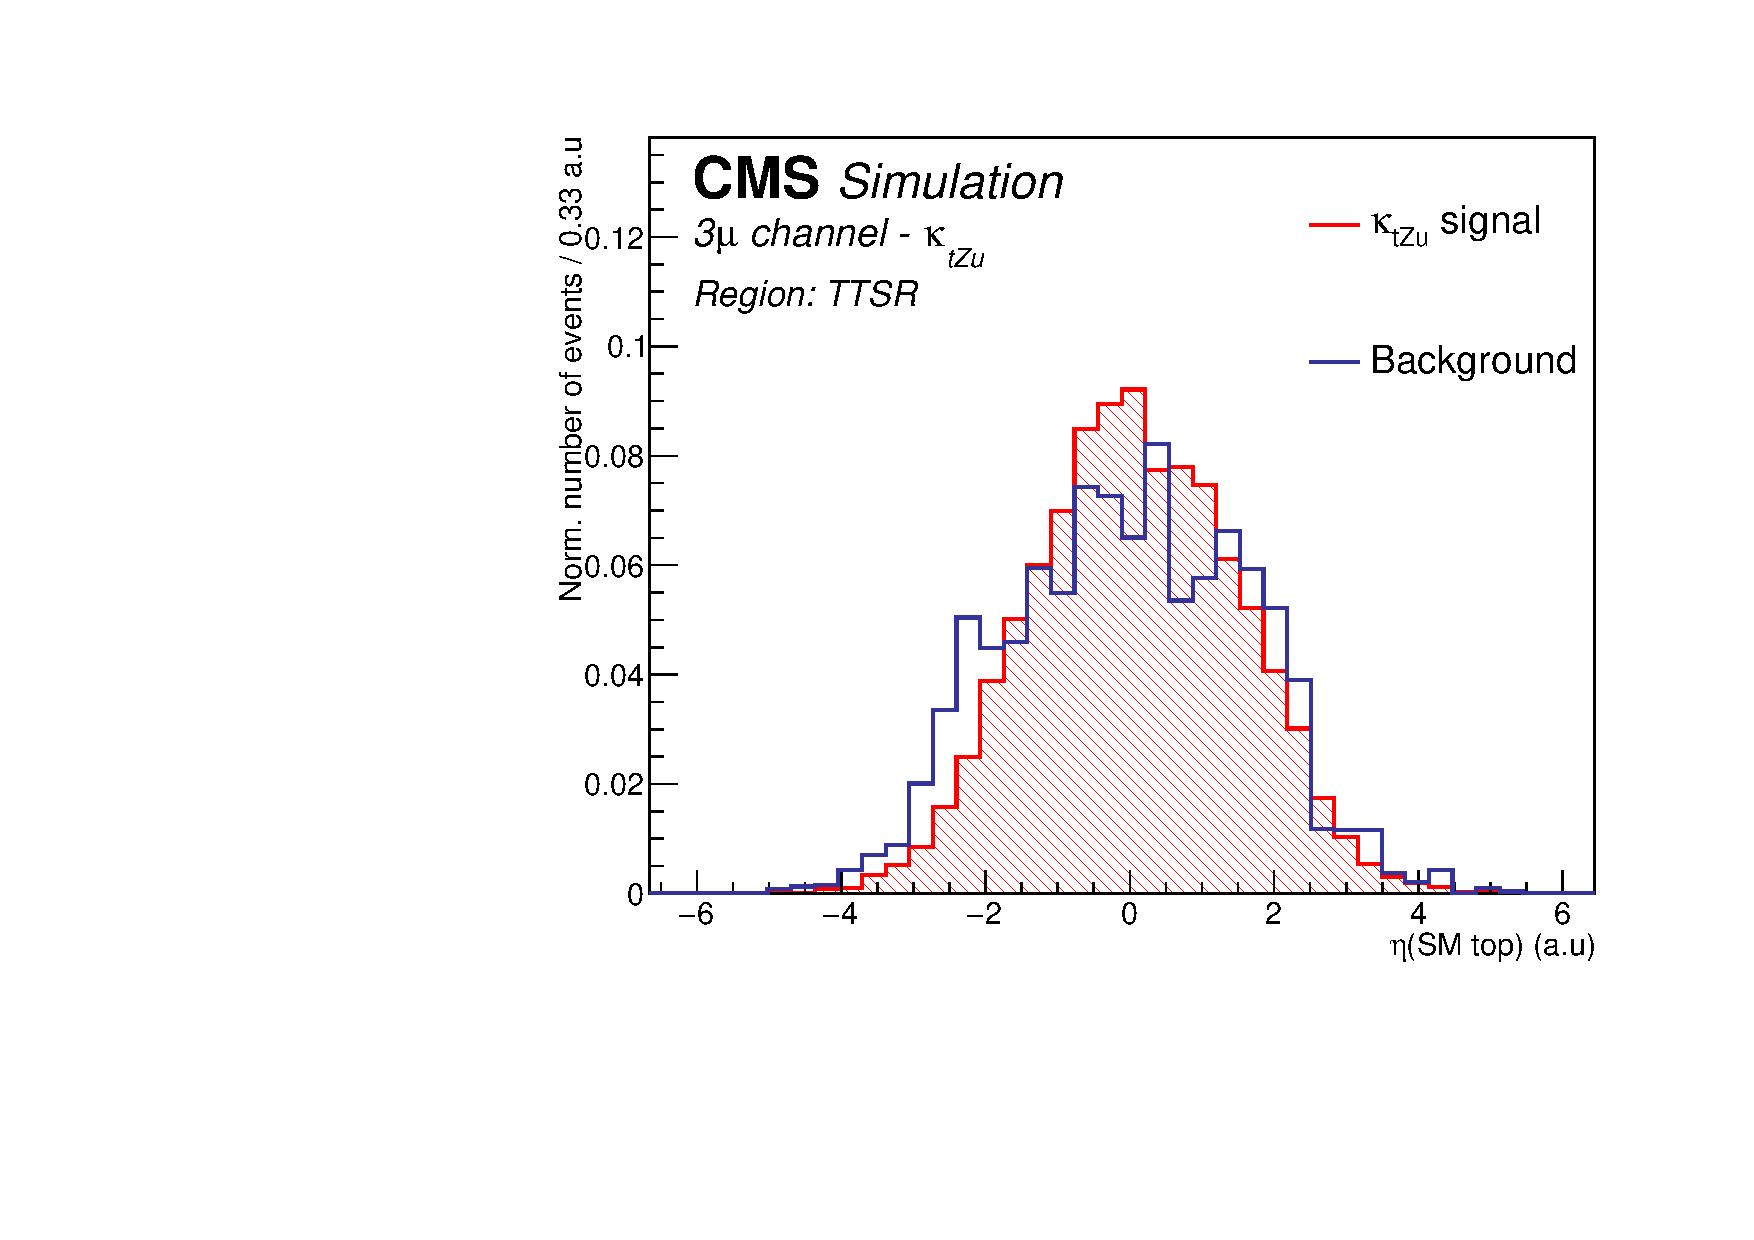
\includegraphics[width=0.3\linewidth]{6_Search/Figures/PlotsTechnics/SMtopetaZuttoppairuuu_norm}
	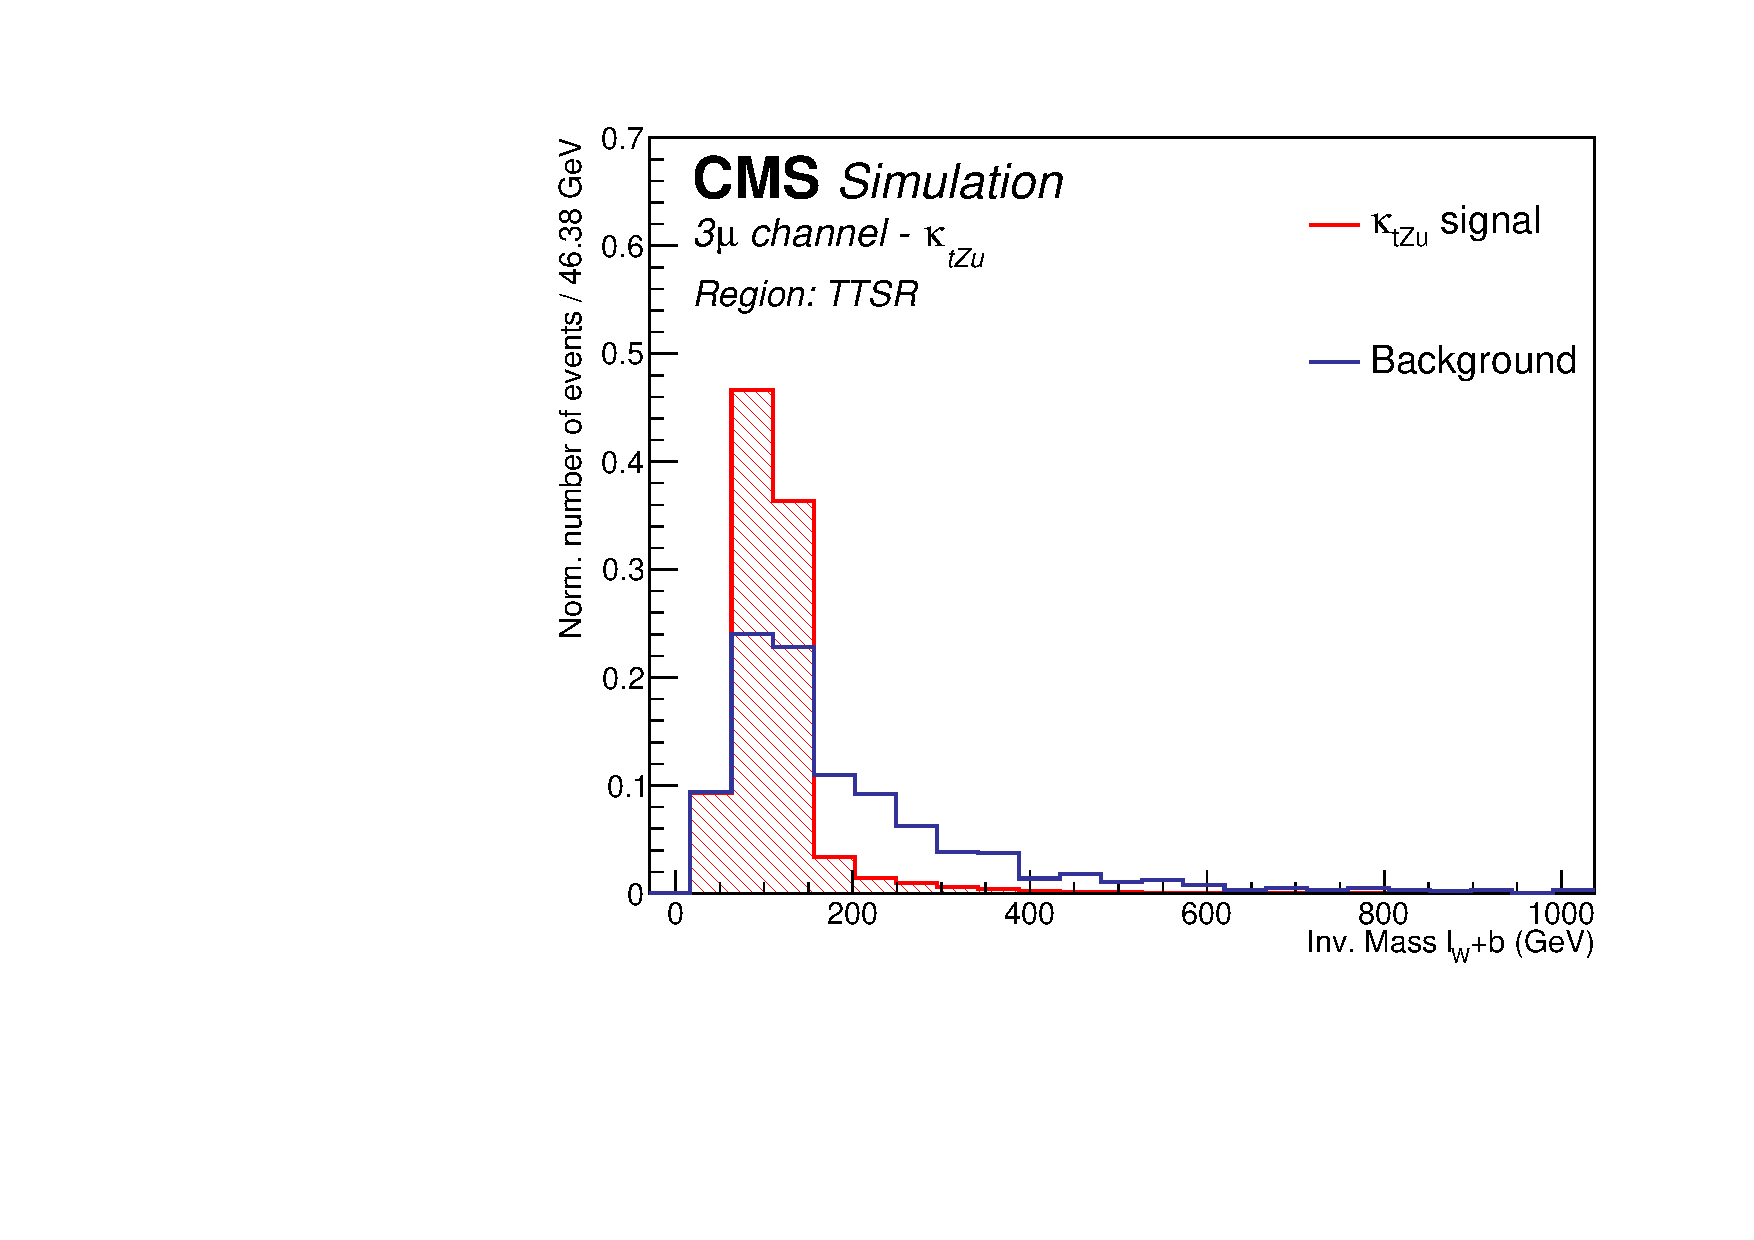
\includegraphics[width=0.3\linewidth]{6_Search/Figures/PlotsTechnics/mlbZuttoppairuuu_norm}
	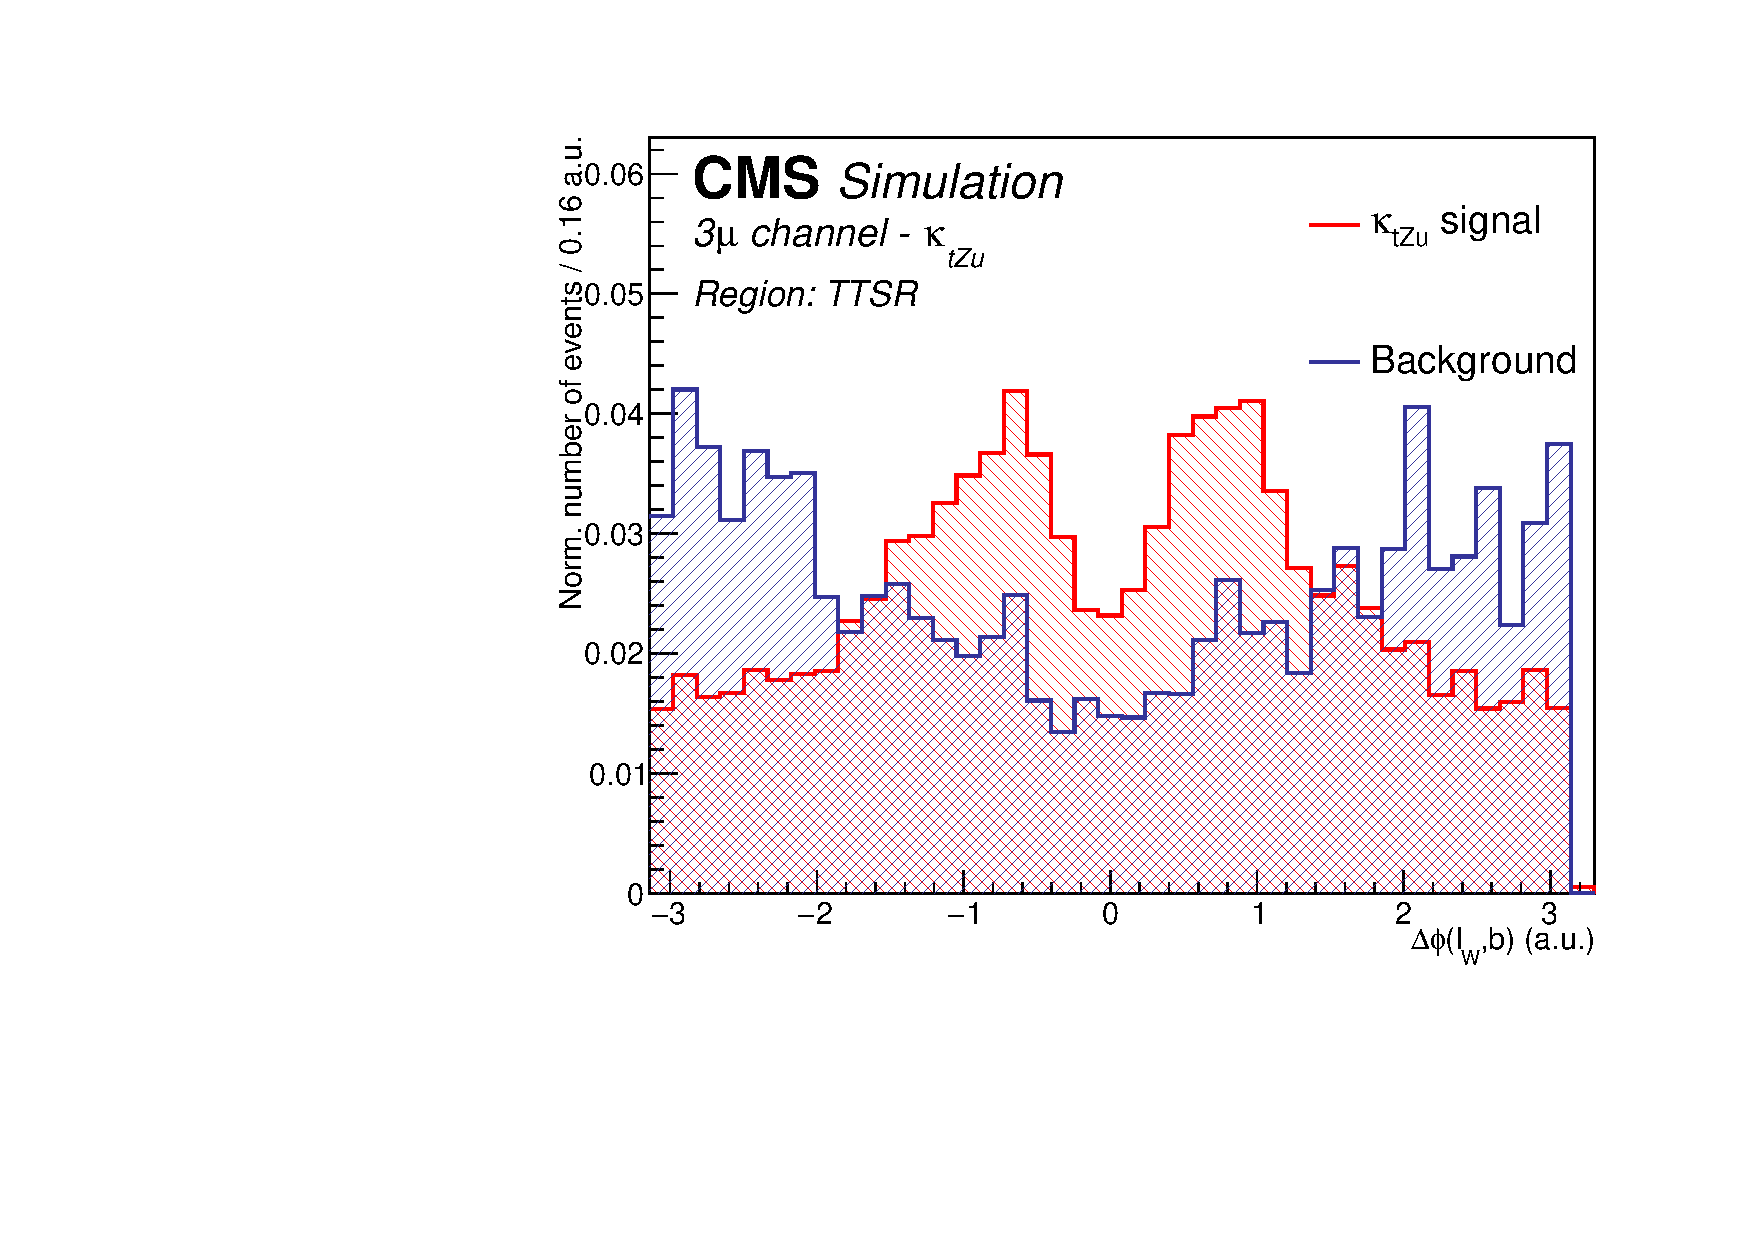
\includegraphics[width=0.3\linewidth]{6_Search/Figures/PlotsTechnics/dPhiWlepbZuttoppairuuu_norm}
	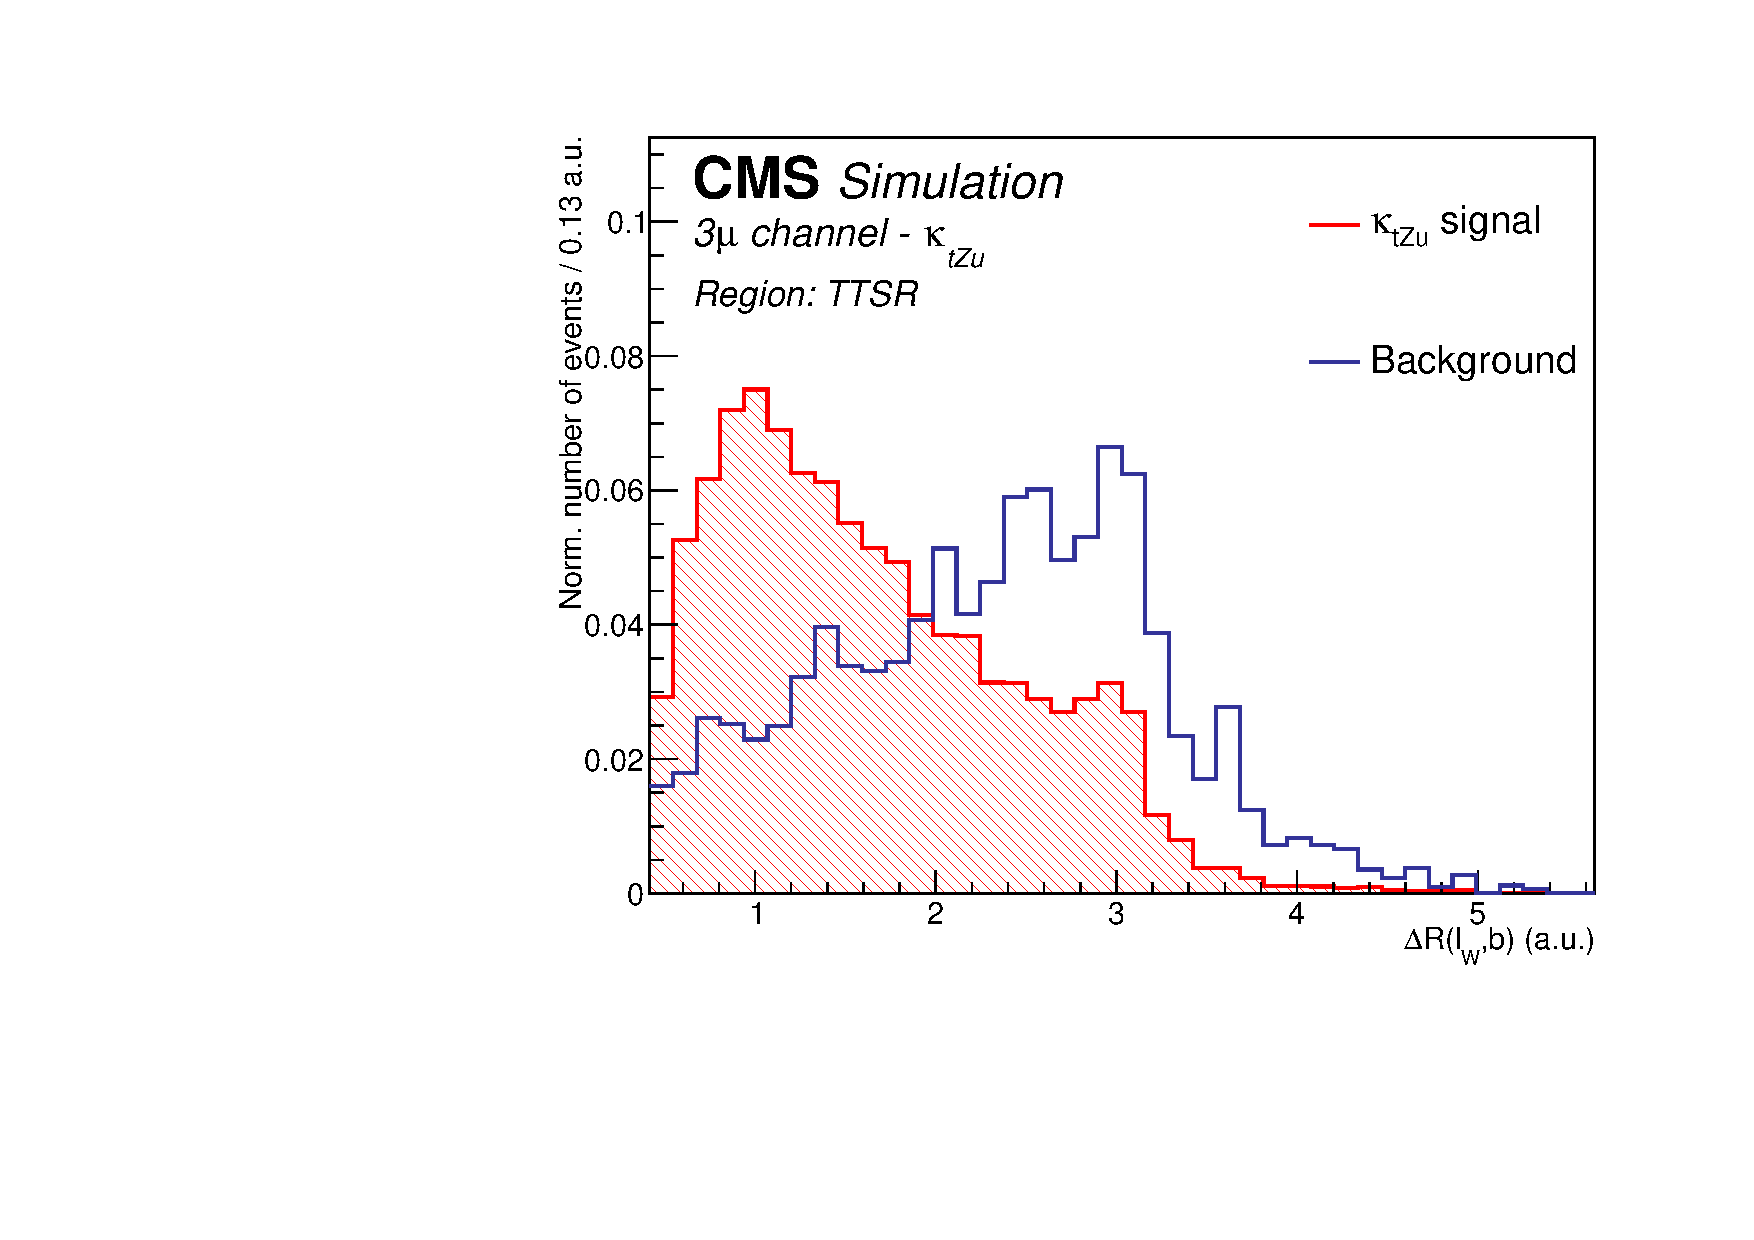
\includegraphics[width=0.3\linewidth]{6_Search/Figures/PlotsTechnics/dRWlepbZuttoppairuuu_norm}
	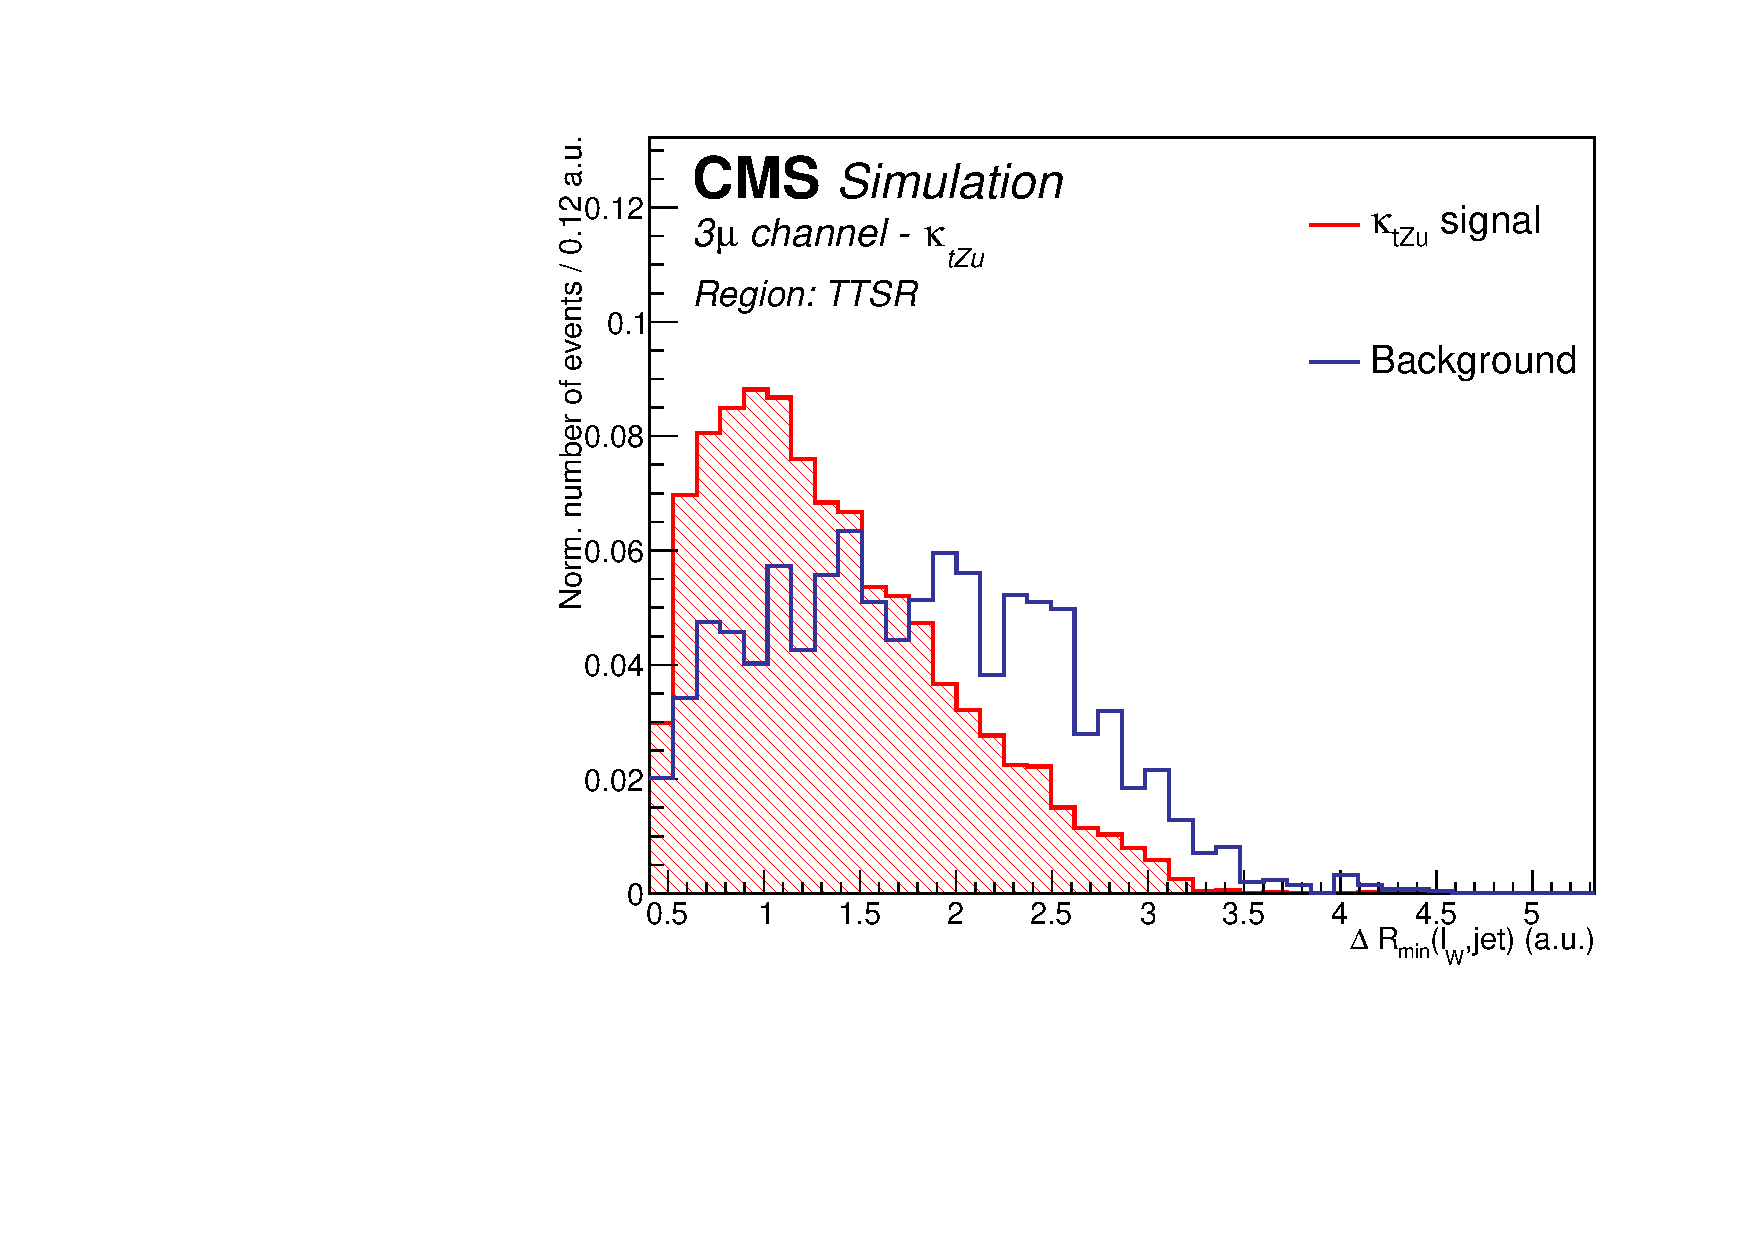
\includegraphics[width=0.3\linewidth]{6_Search/Figures/PlotsTechnics/deltaRWlepJet_minZuttoppairuuu_norm}
		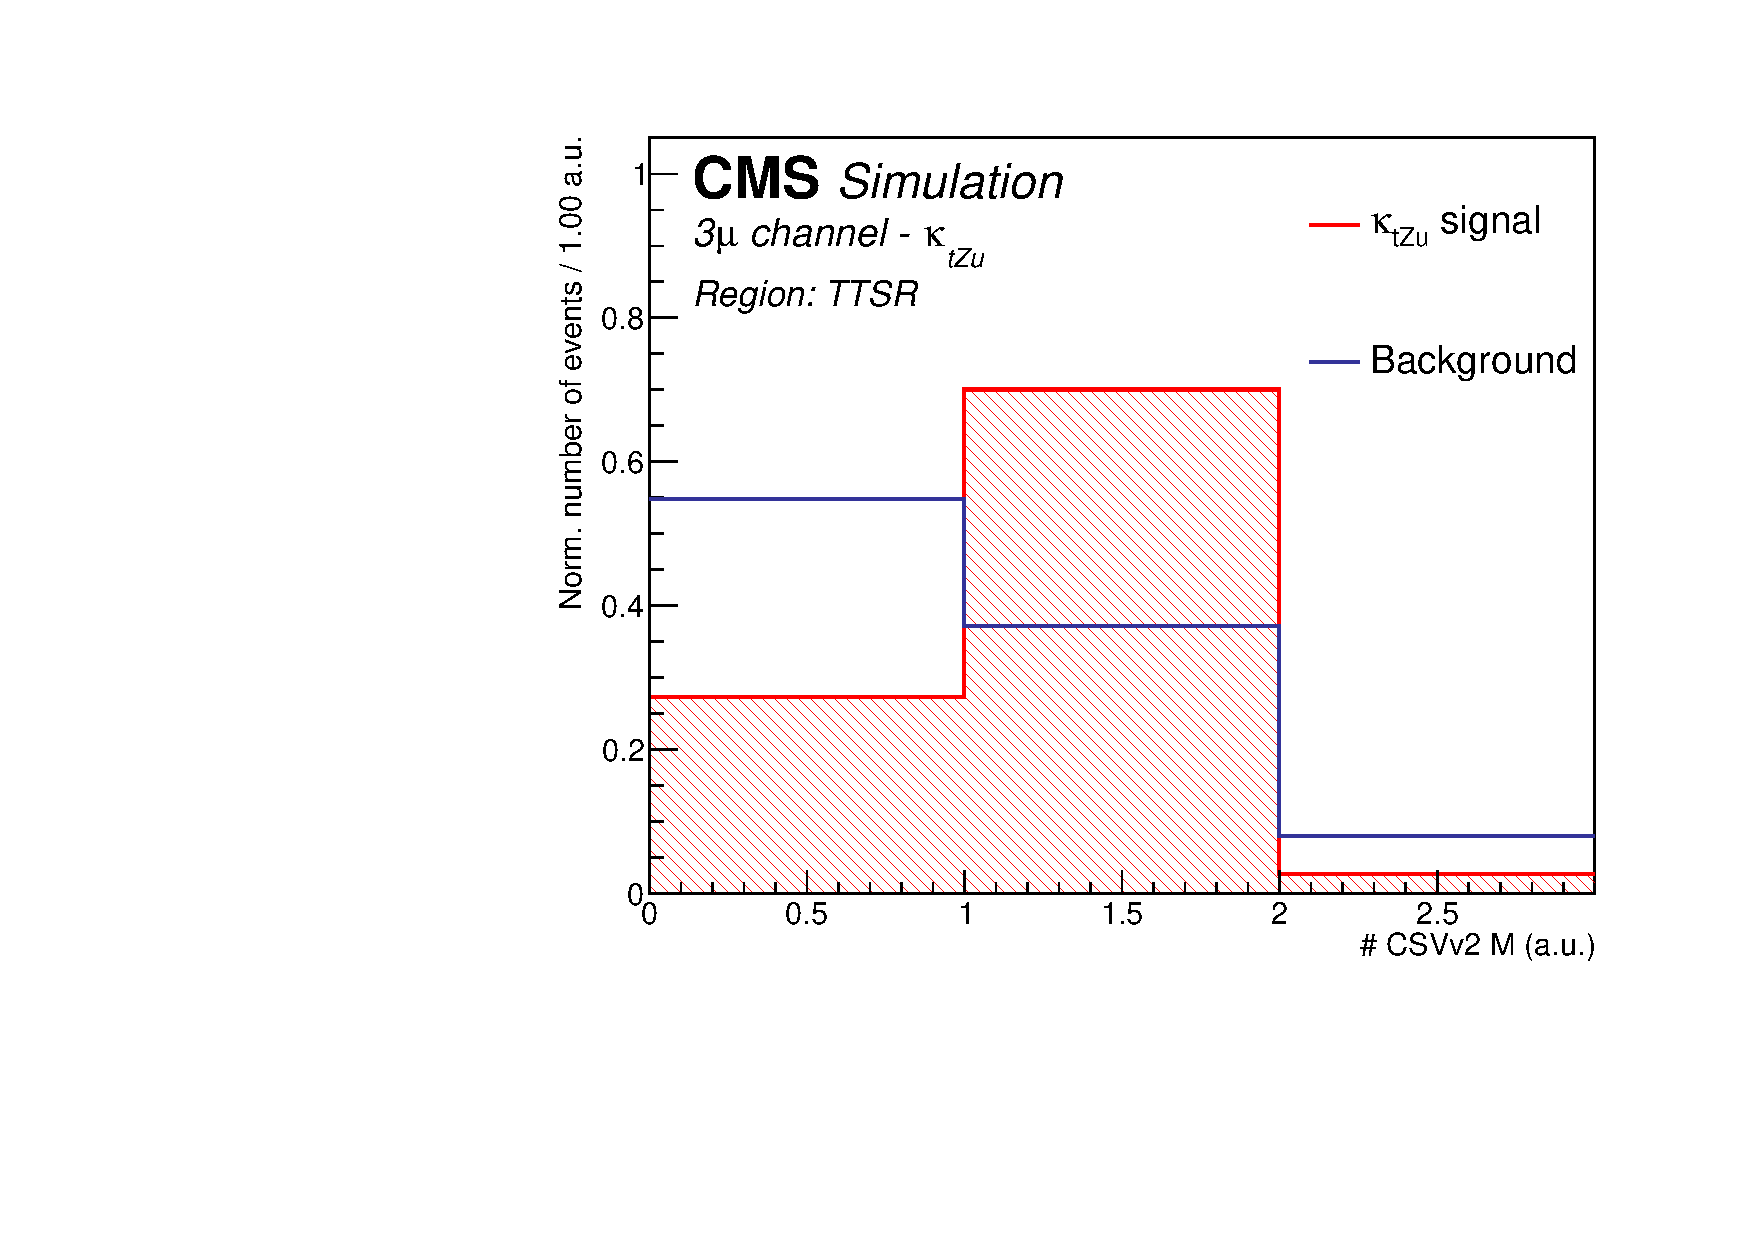
\includegraphics[width=0.3\linewidth]{6_Search/Figures/PlotsTechnics/NJets_CSVv2MZuttoppairuuu_norm}
	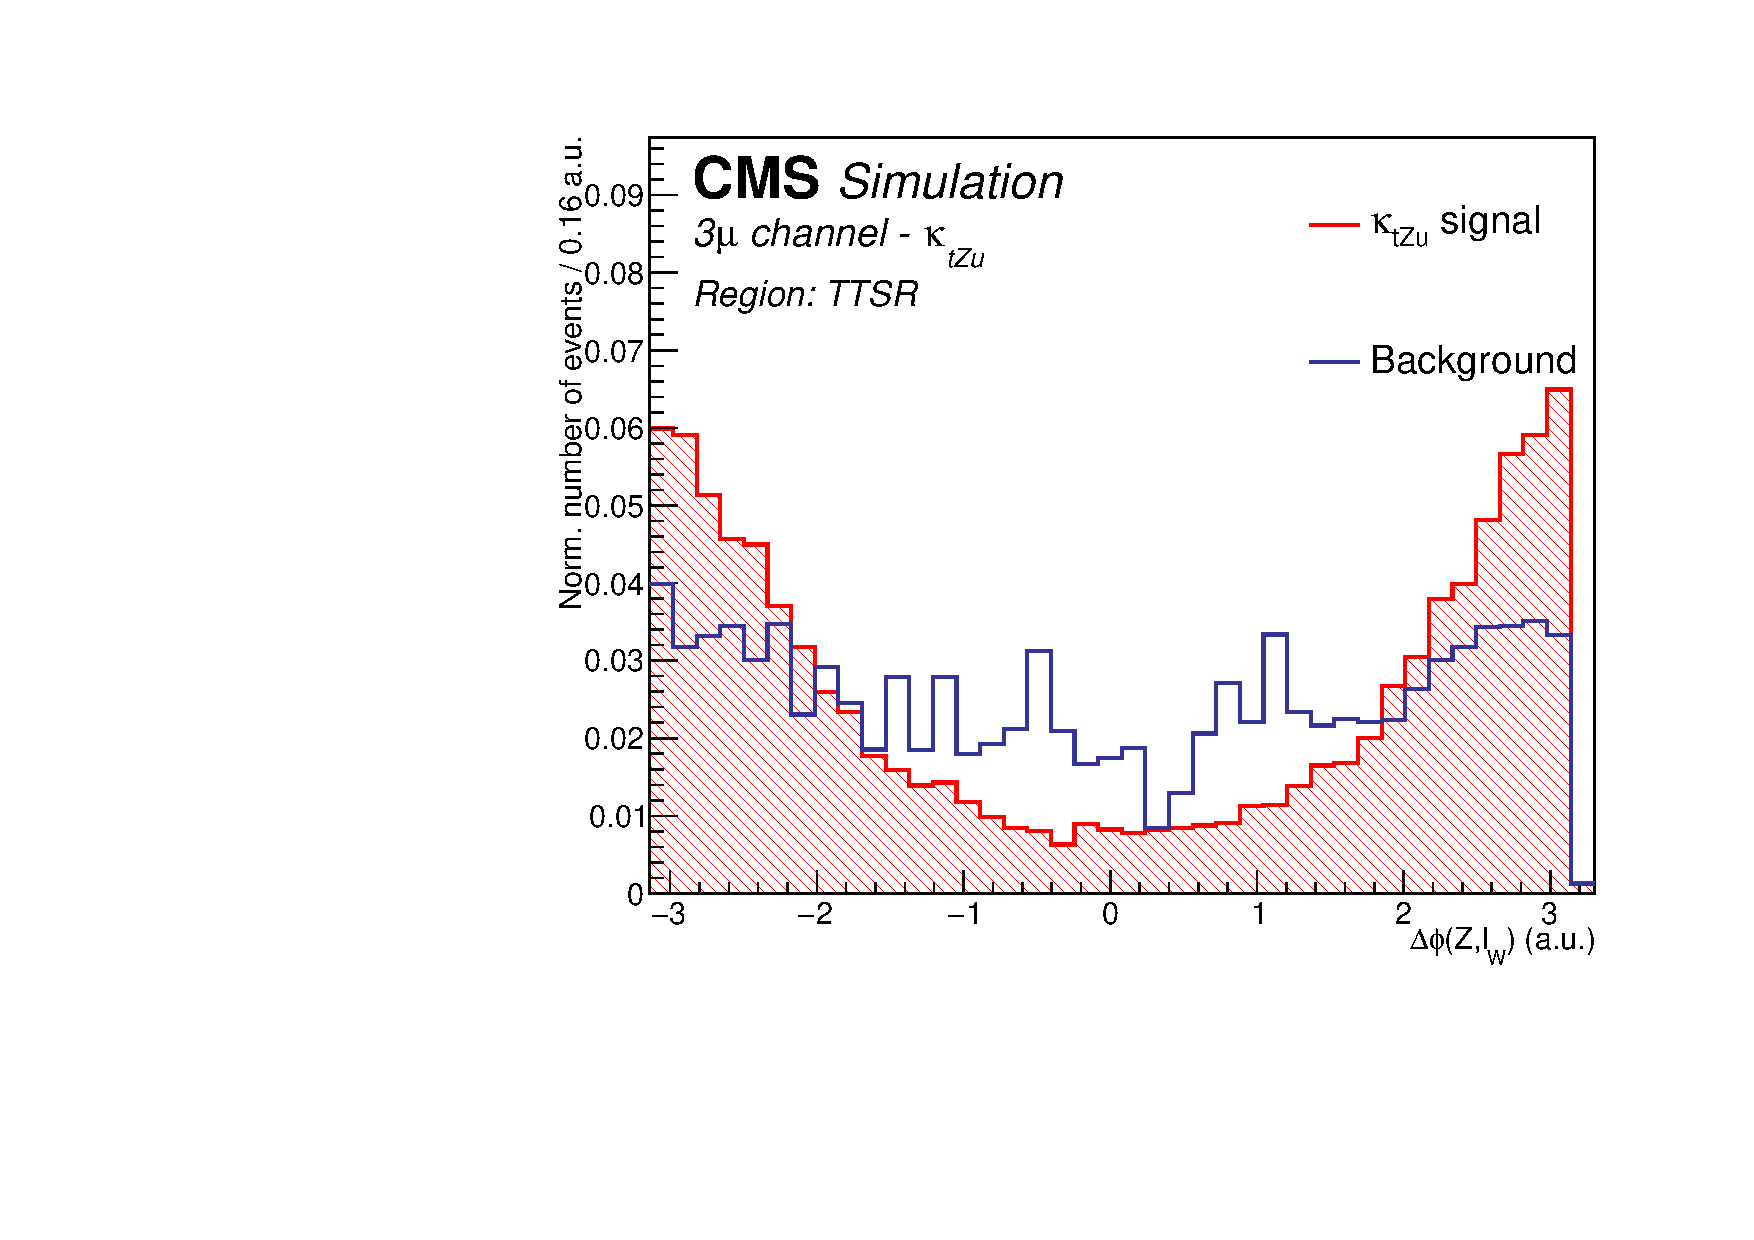
\includegraphics[width=0.3\linewidth]{6_Search/Figures/PlotsTechnics/dPhiZWlepZuttoppairuuu_norm}
	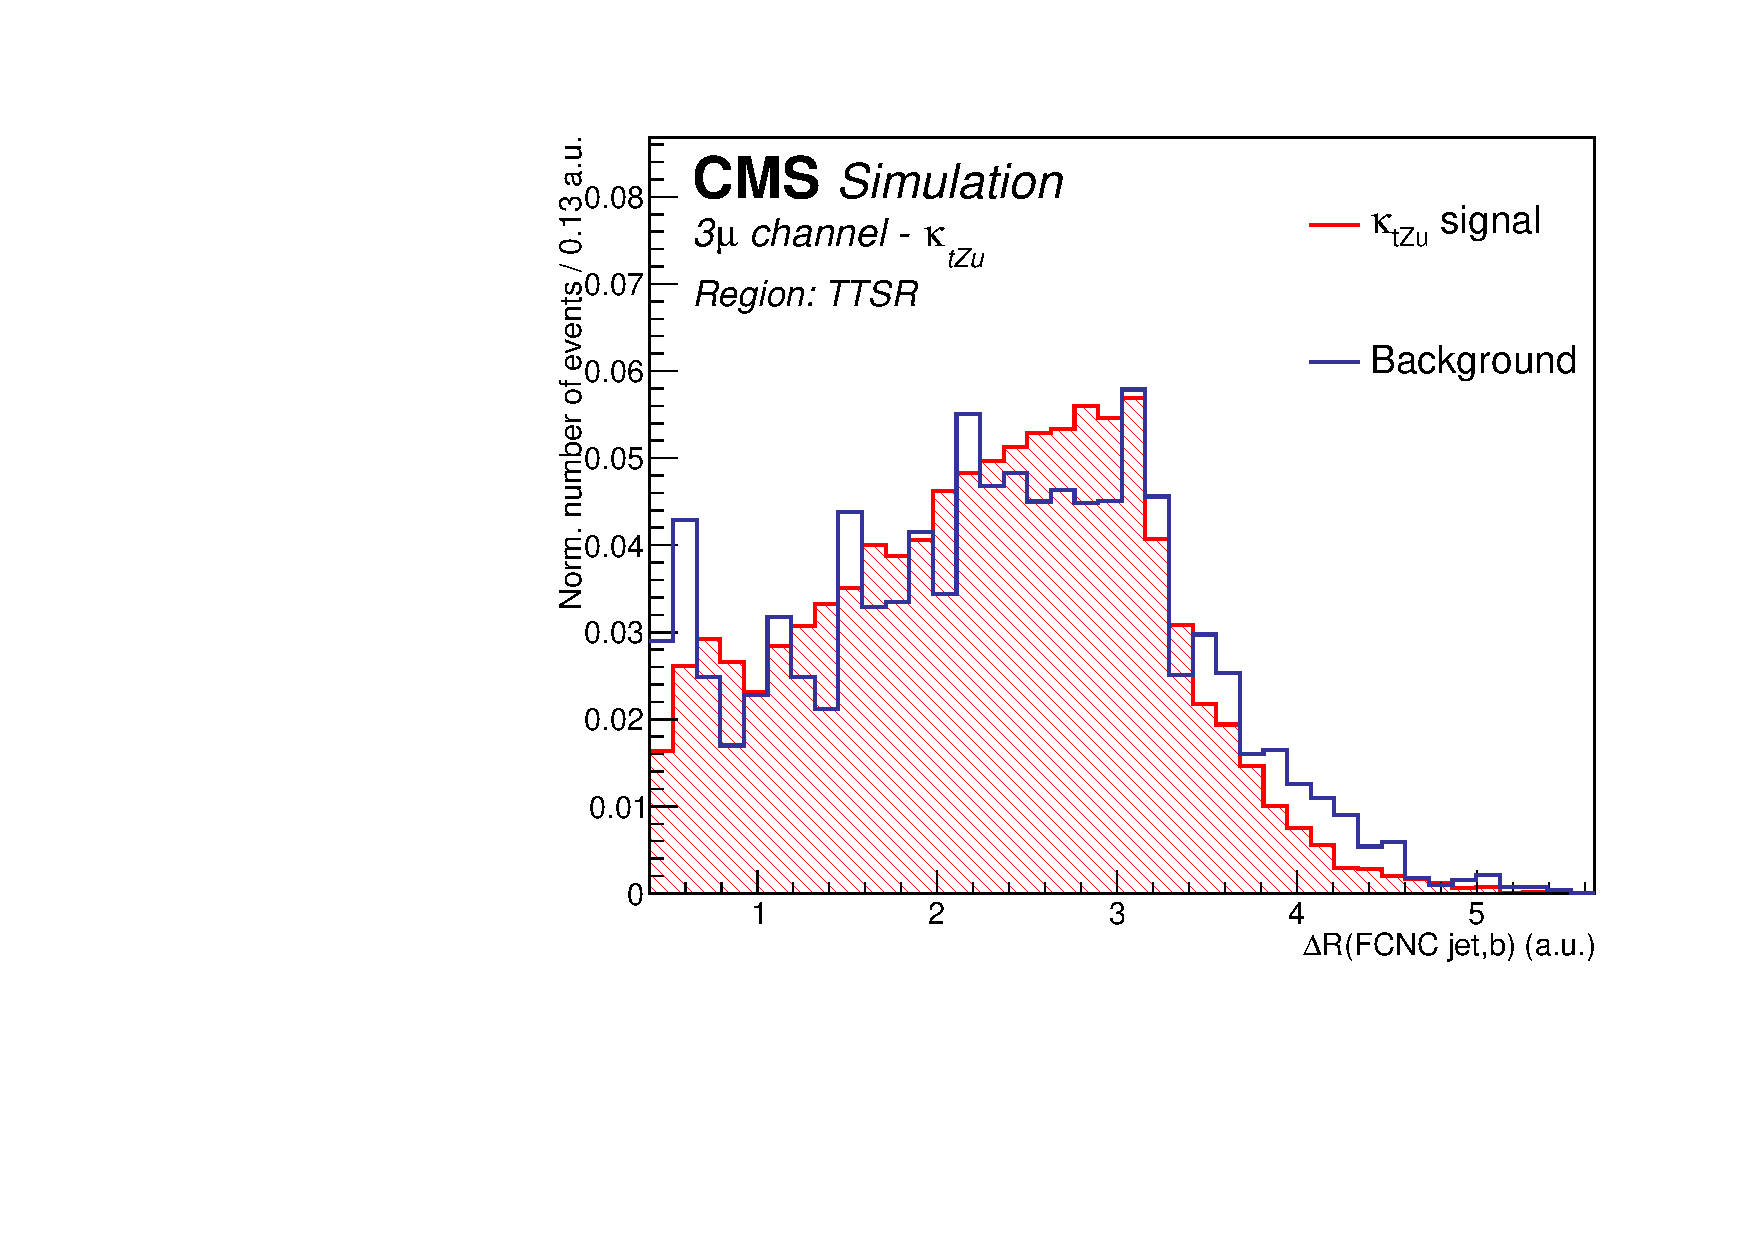
\includegraphics[width=0.3\linewidth]{6_Search/Figures/PlotsTechnics/dRSMjetLightjetZuttoppairuuu_norm}
	\caption{The normalised distributions for input variables for reconstructing the multivariate discriminator in the \TTSR\ for the \Zut\ vertex, in the \mumumu\ lepton channel. The contribution of the \NPL\ background is not included.}
	\label{fig:toppairZutnormalized}
\end{figure}

\newpage
In \fig{fig:correlationsigzuttoppair}, the correlations between the input variables used for training and creating the multivariate discriminating variable are shown. In general, there is only a small correlation between the variables, with the exception of the distances and mass of the components of the top quarks. 
\begin{figure}[htbp]
	\centering
	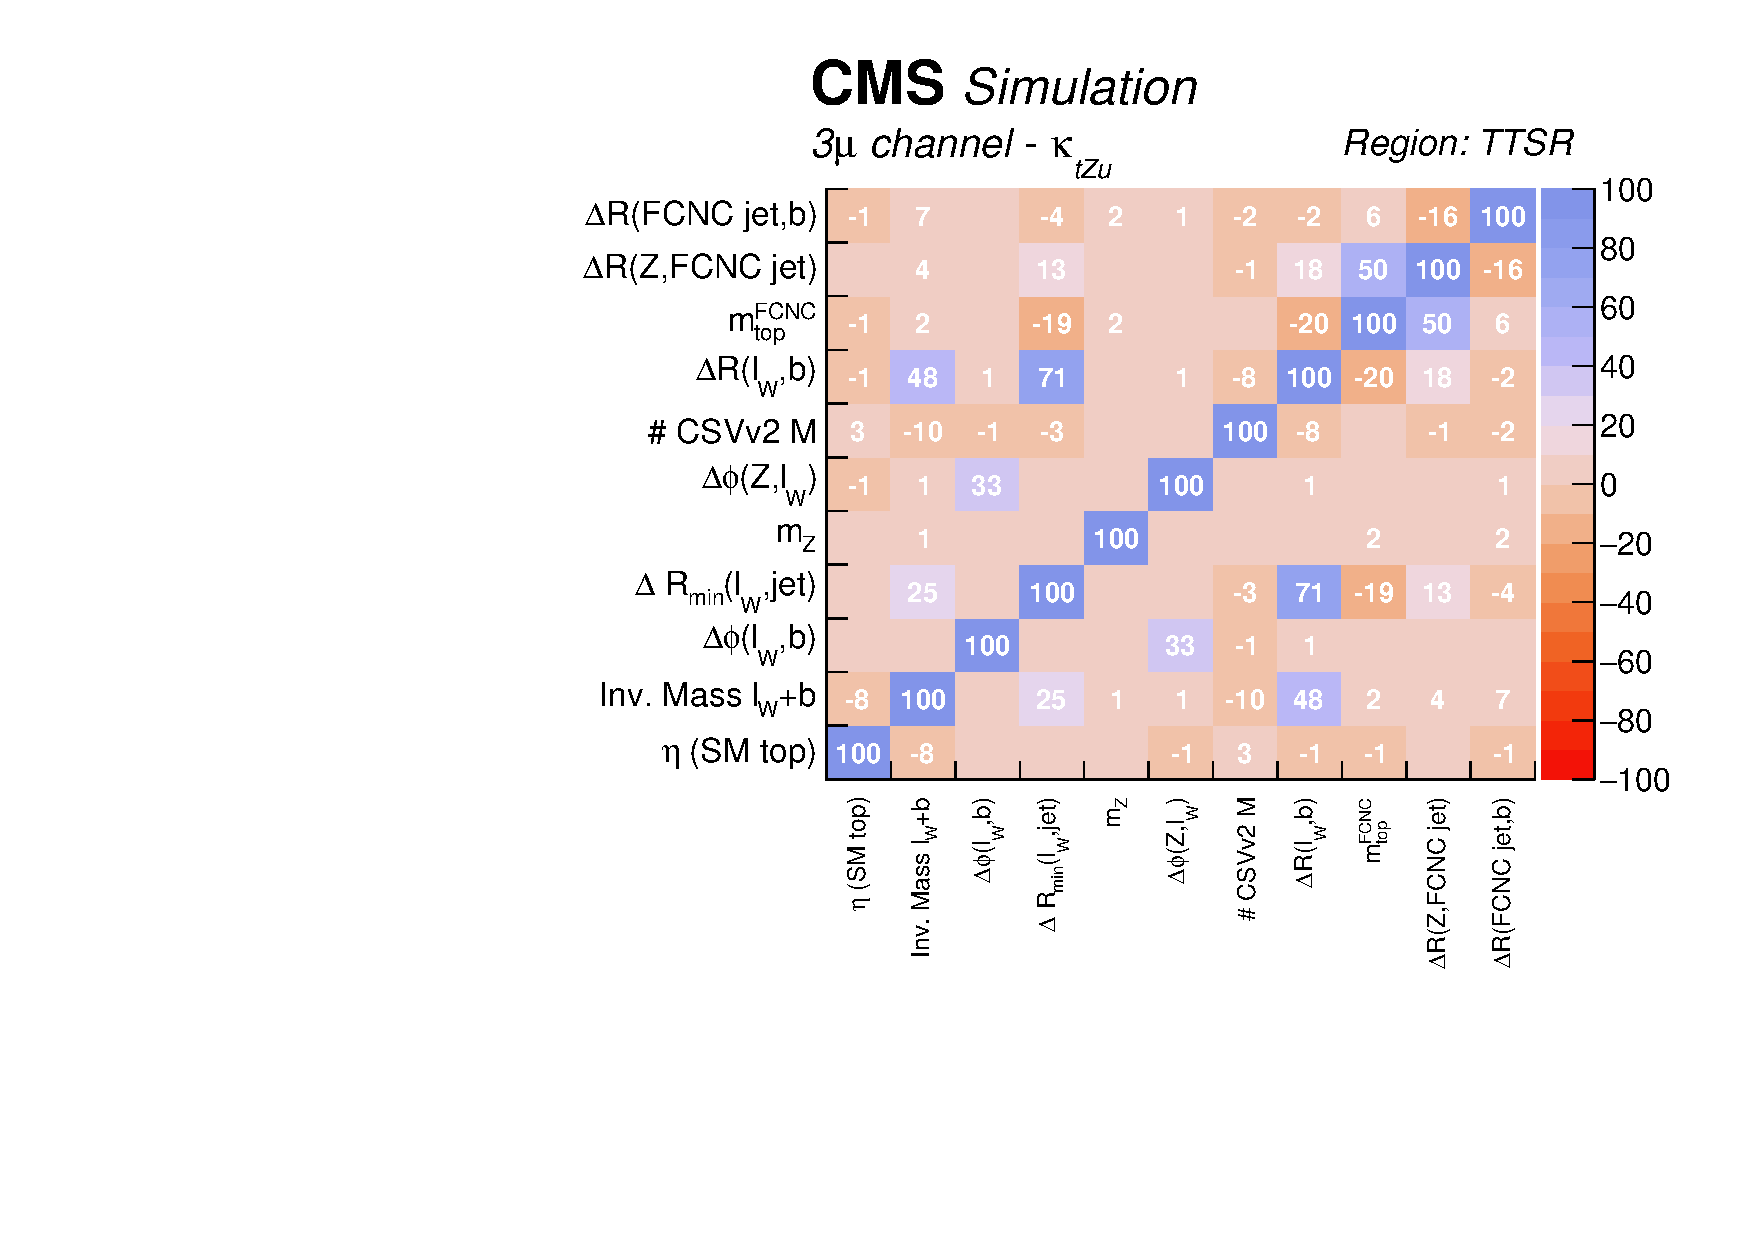
\includegraphics[width=0.49\linewidth]{6_Search/Figures/PlotsTechnics/correlationsigZuttoppairuuu}
	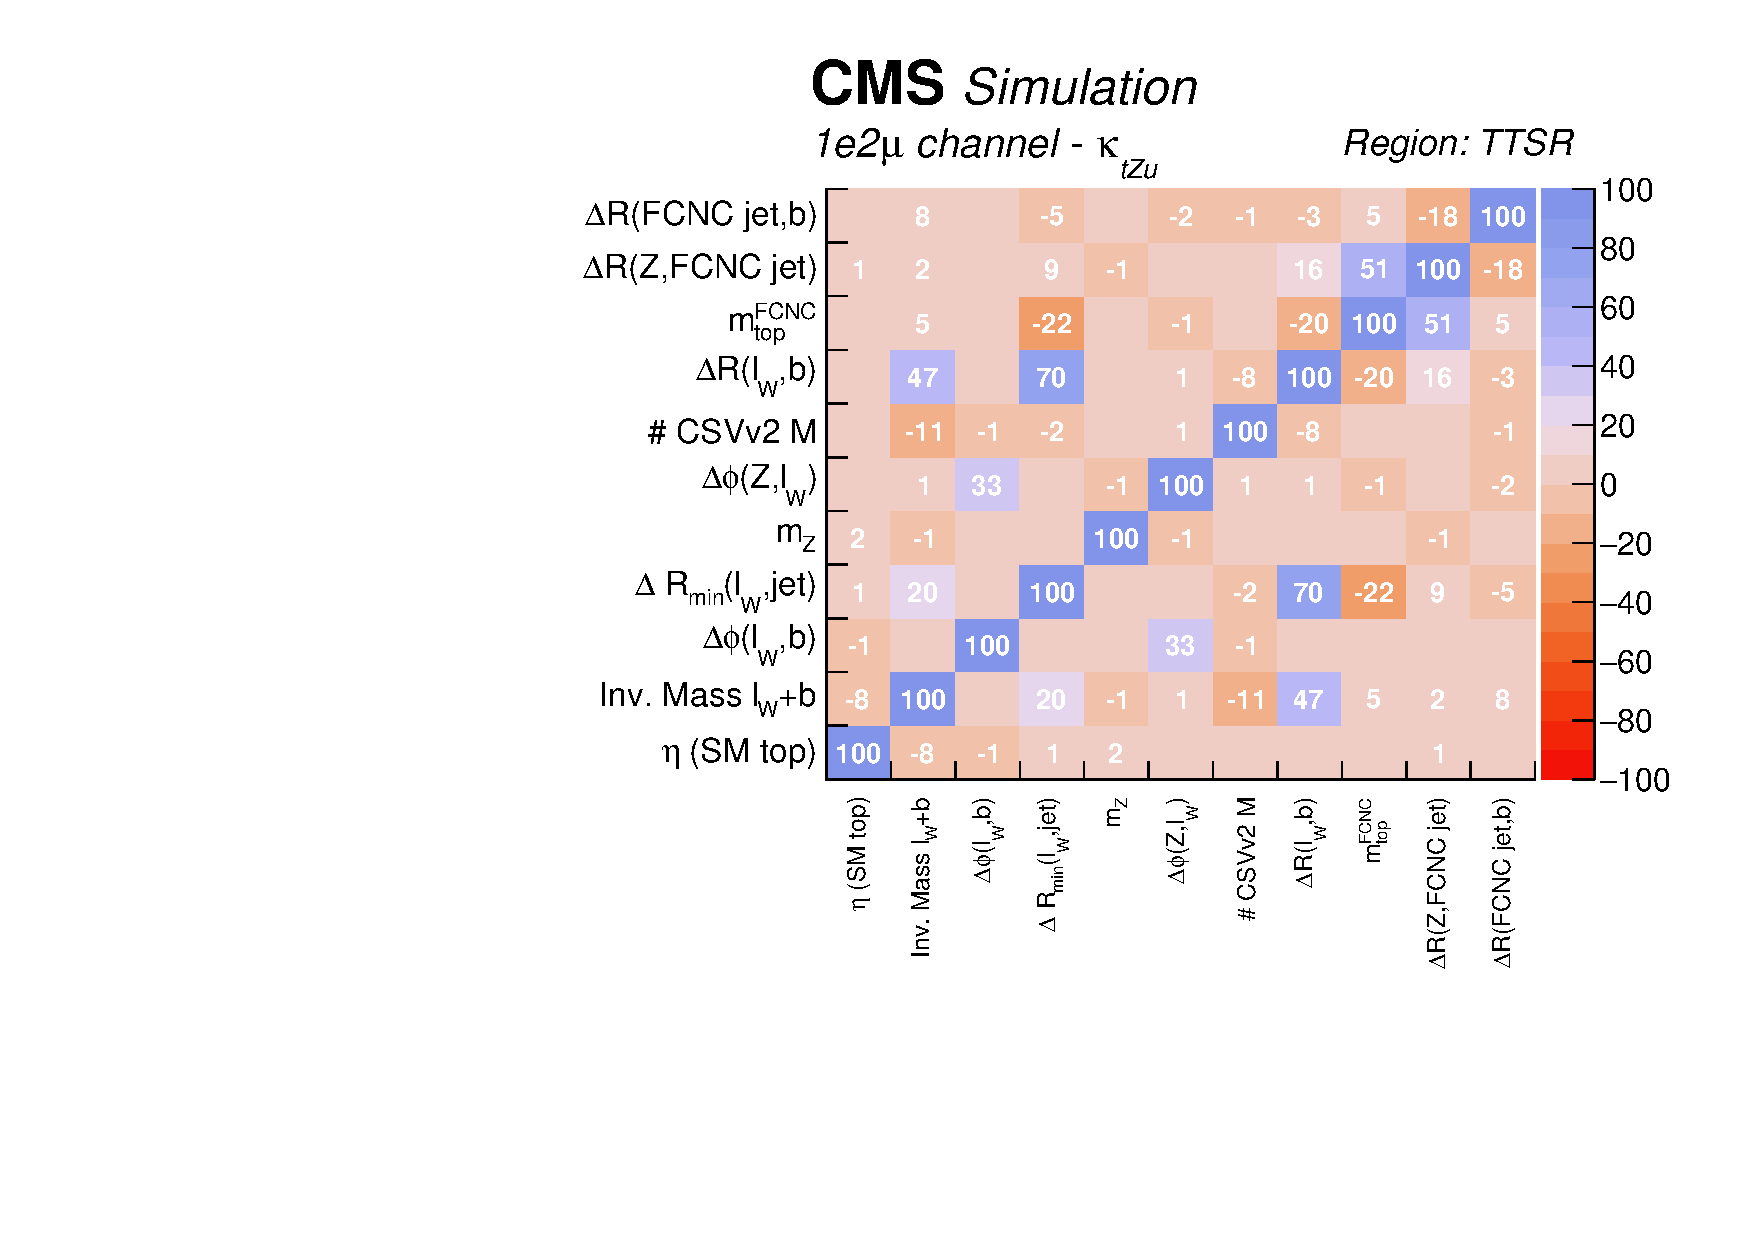
\includegraphics[width=0.49\linewidth]{6_Search/Figures/PlotsTechnics/correlationsigZuttoppairuue}
	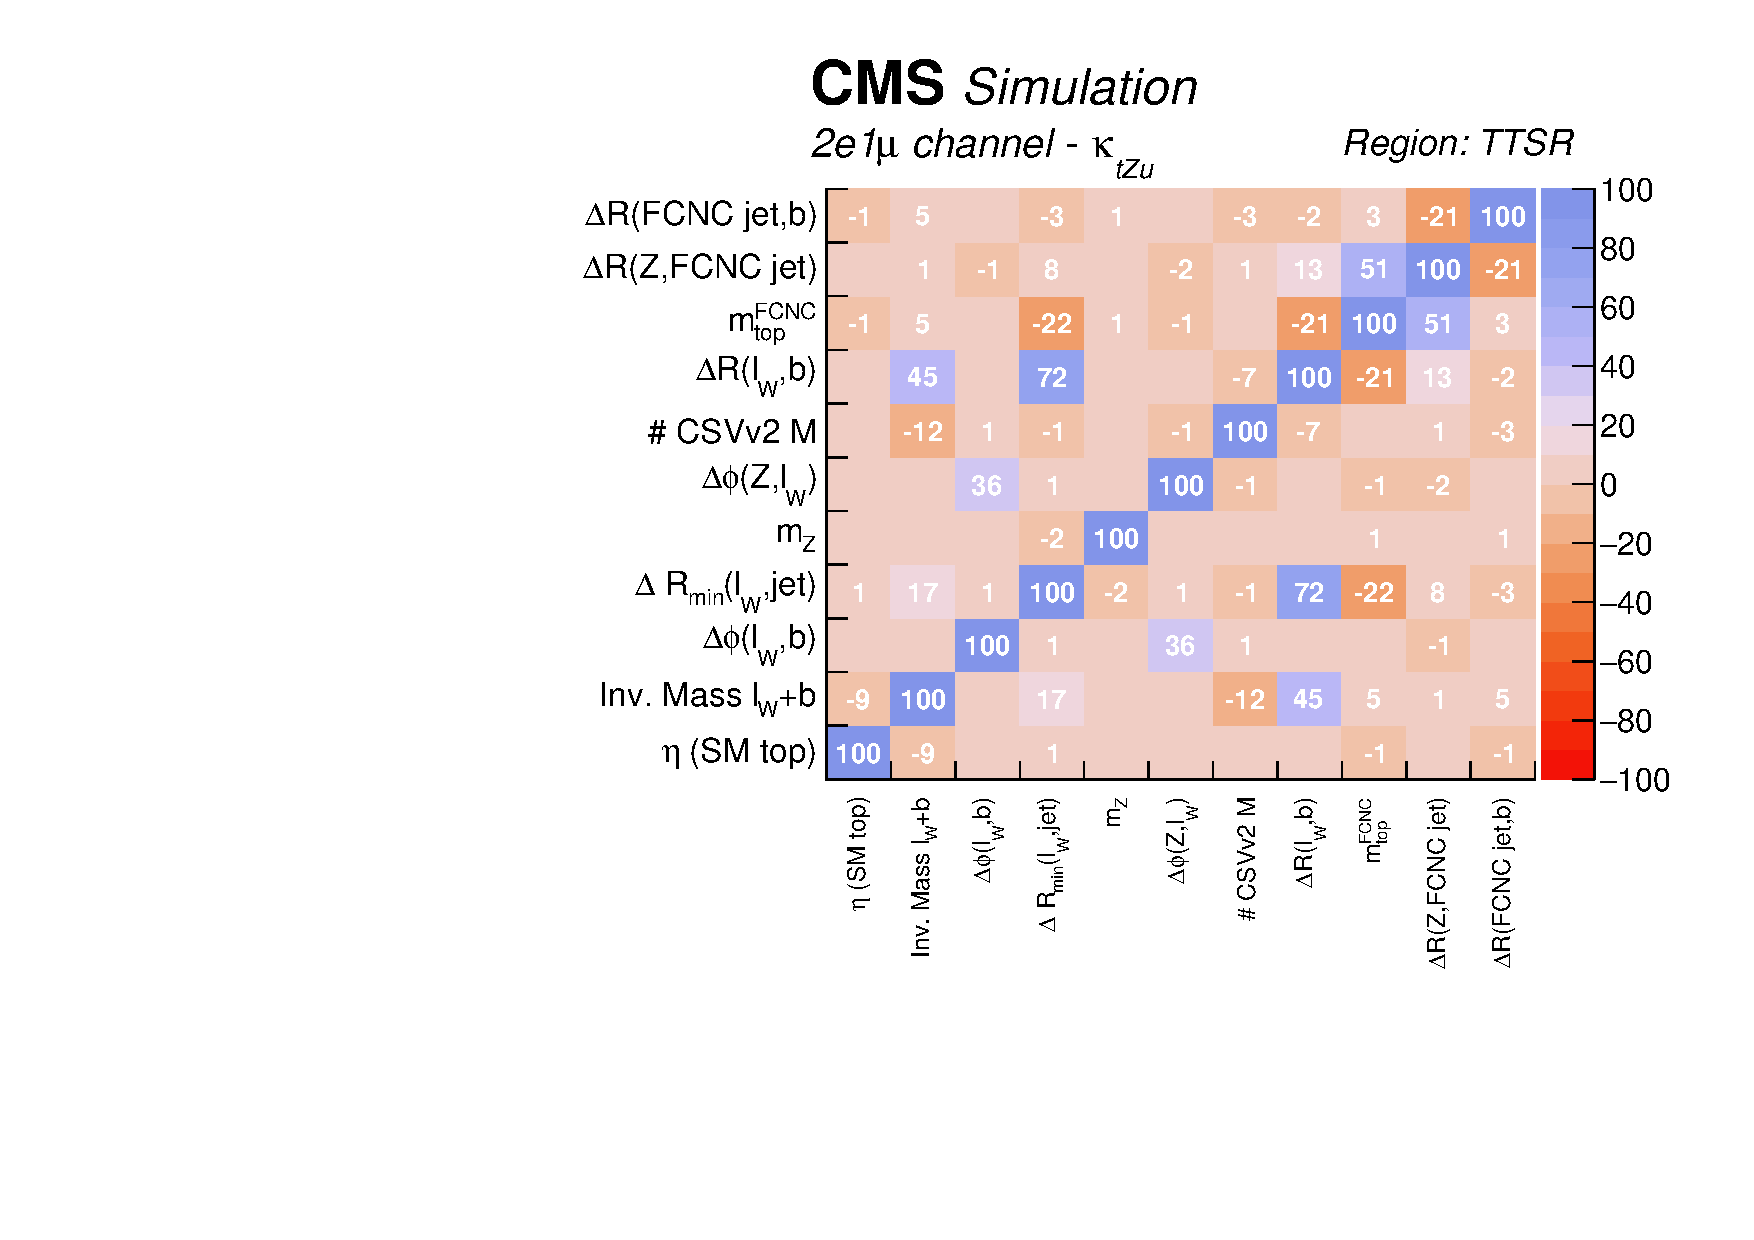
\includegraphics[width=0.49\linewidth]{6_Search/Figures/PlotsTechnics/correlationsigZuttoppaireeu}
	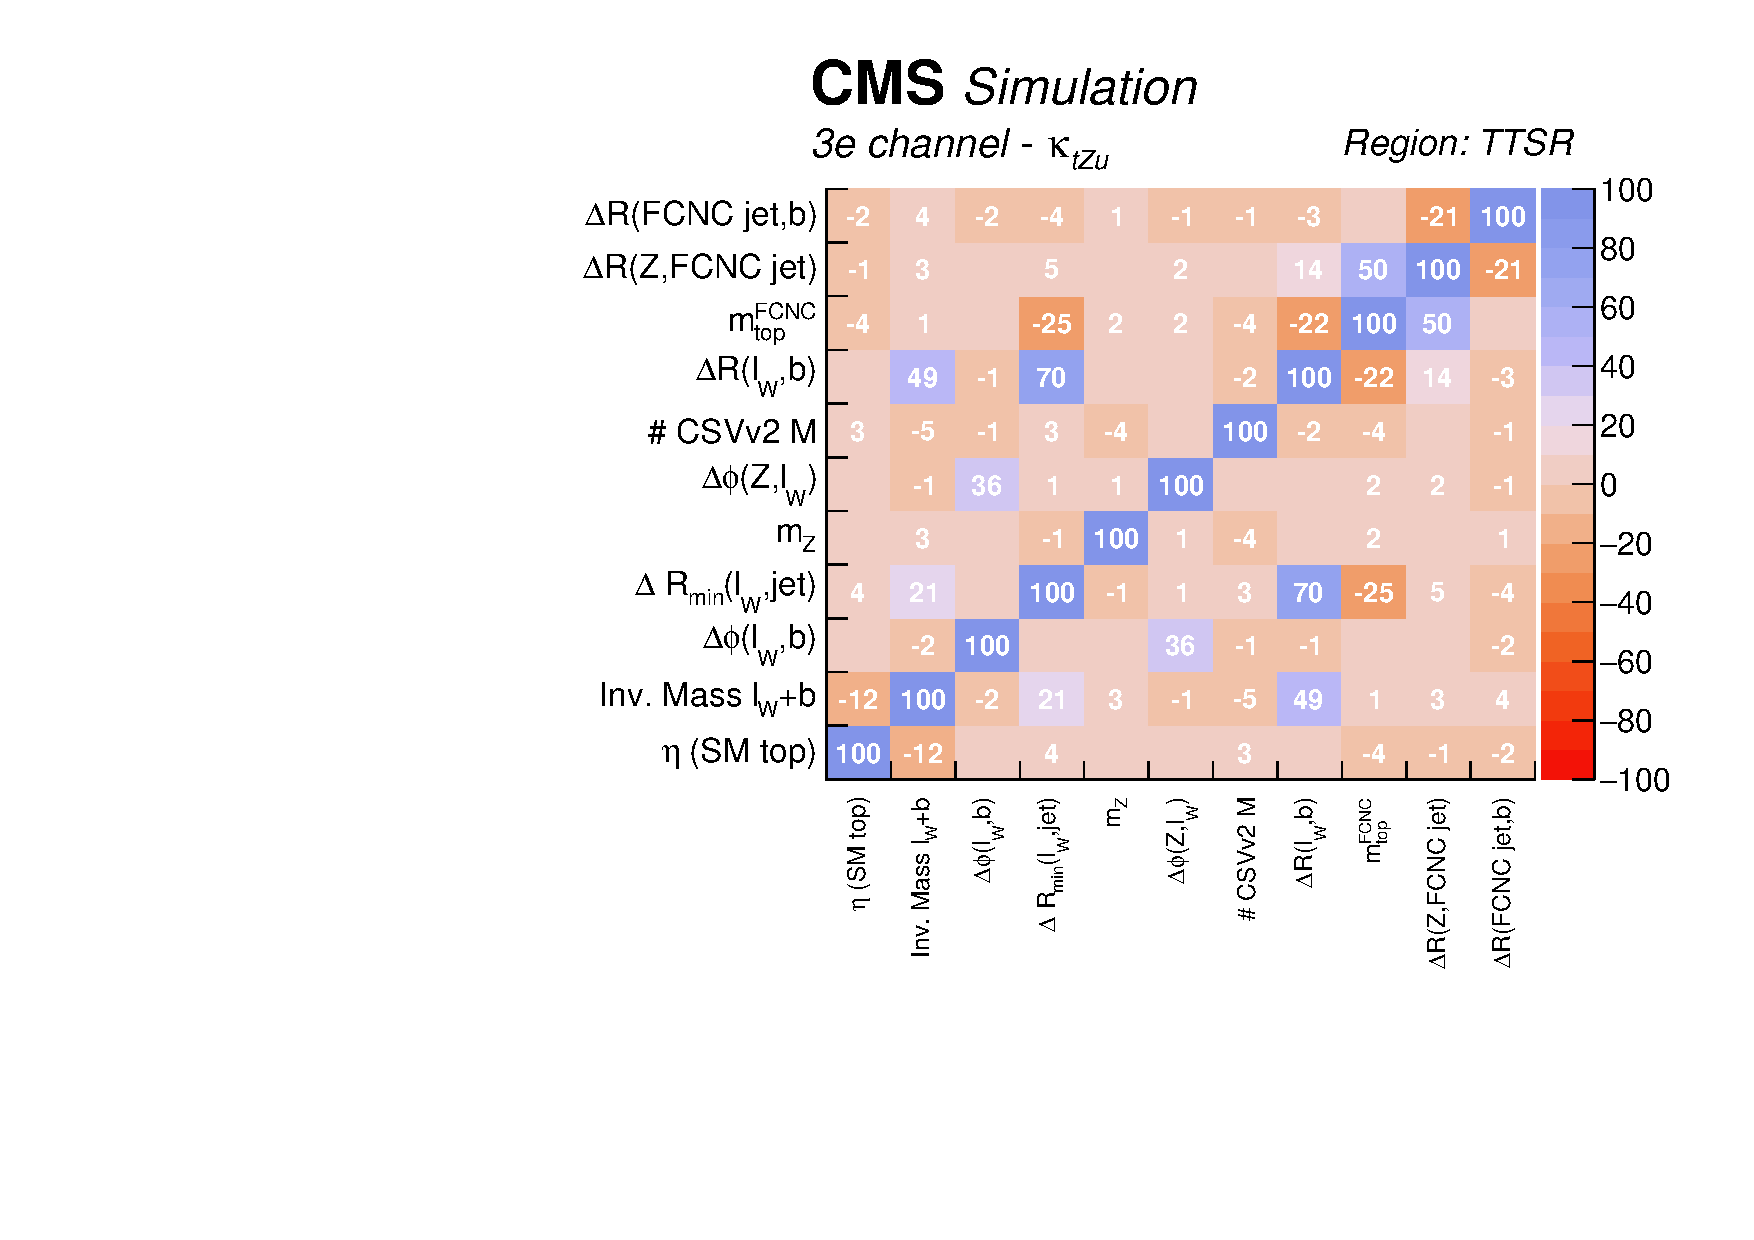
\includegraphics[width=0.49\linewidth]{6_Search/Figures/PlotsTechnics/correlationsigZuttoppaireee}
	\caption{The correlations between the input variables used to create the multivariate discriminant in the \TTSR, for the \Zut\ signal. For the \mumumu\ (left,top), \emumu\ (right,top), \eemu\ (left, bottom) and \eee\ (right,bottom) three-lepton channel.}
	\label{fig:correlationsigzuttoppair}
\end{figure}

\clearpage
The resulting multivariate discriminator D for this region is shown in \fig{fig:sigvsbkgtestzuttoppair} for all three-lepton channels. Again, there is a clear discrimination between the FCNC signal and the backgrounds, and the testing and training samples agree with each other. Hence, there is no overtraining observed. The ROC curves are shown in \fig{fig:roczuttoppair}, where the testing sample is slightly under the training sample. However, a large separation power is still obtained for signal and background like events. 
\begin{figure}[htbp]
	\centering
	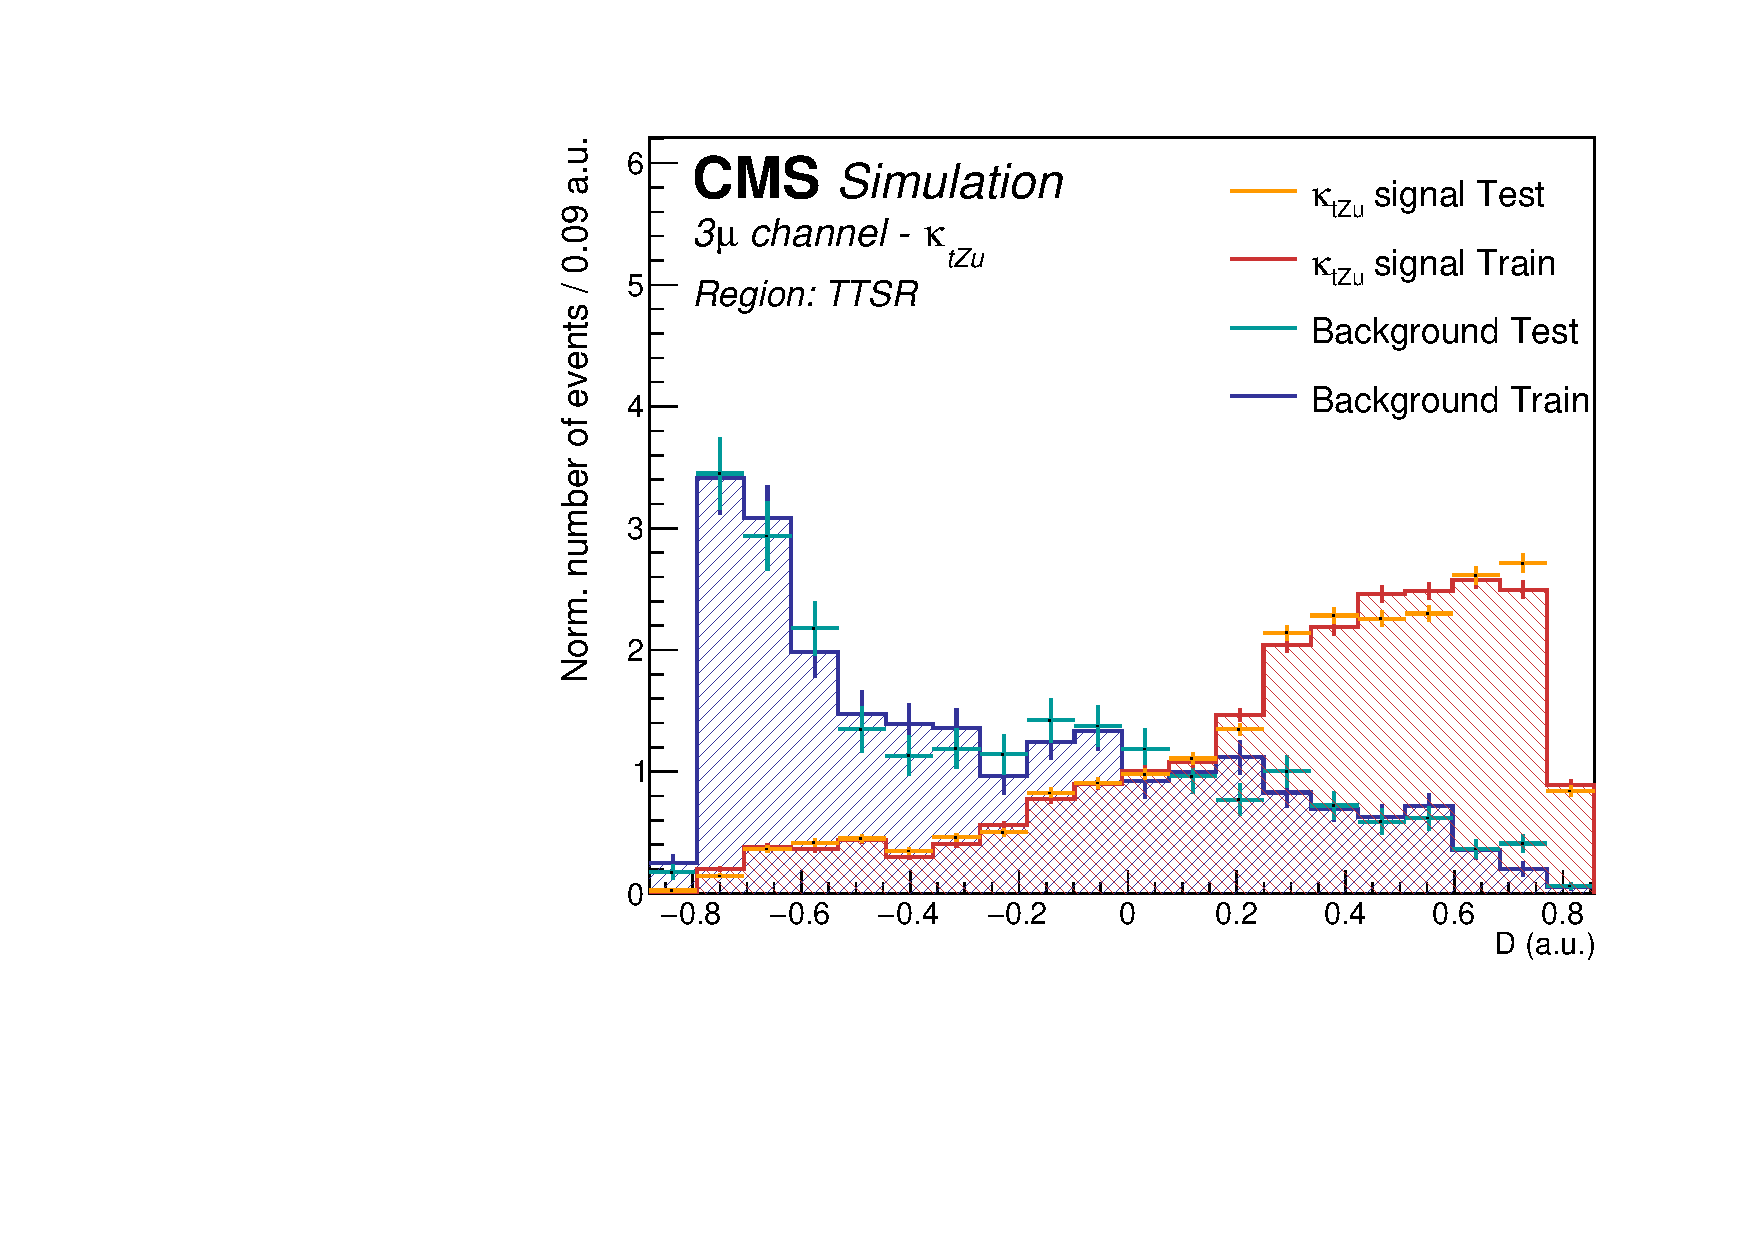
\includegraphics[width=0.49\linewidth]{6_Search/Figures/PlotsTechnics/SigVsBkgTestZuttoppairuuu}
	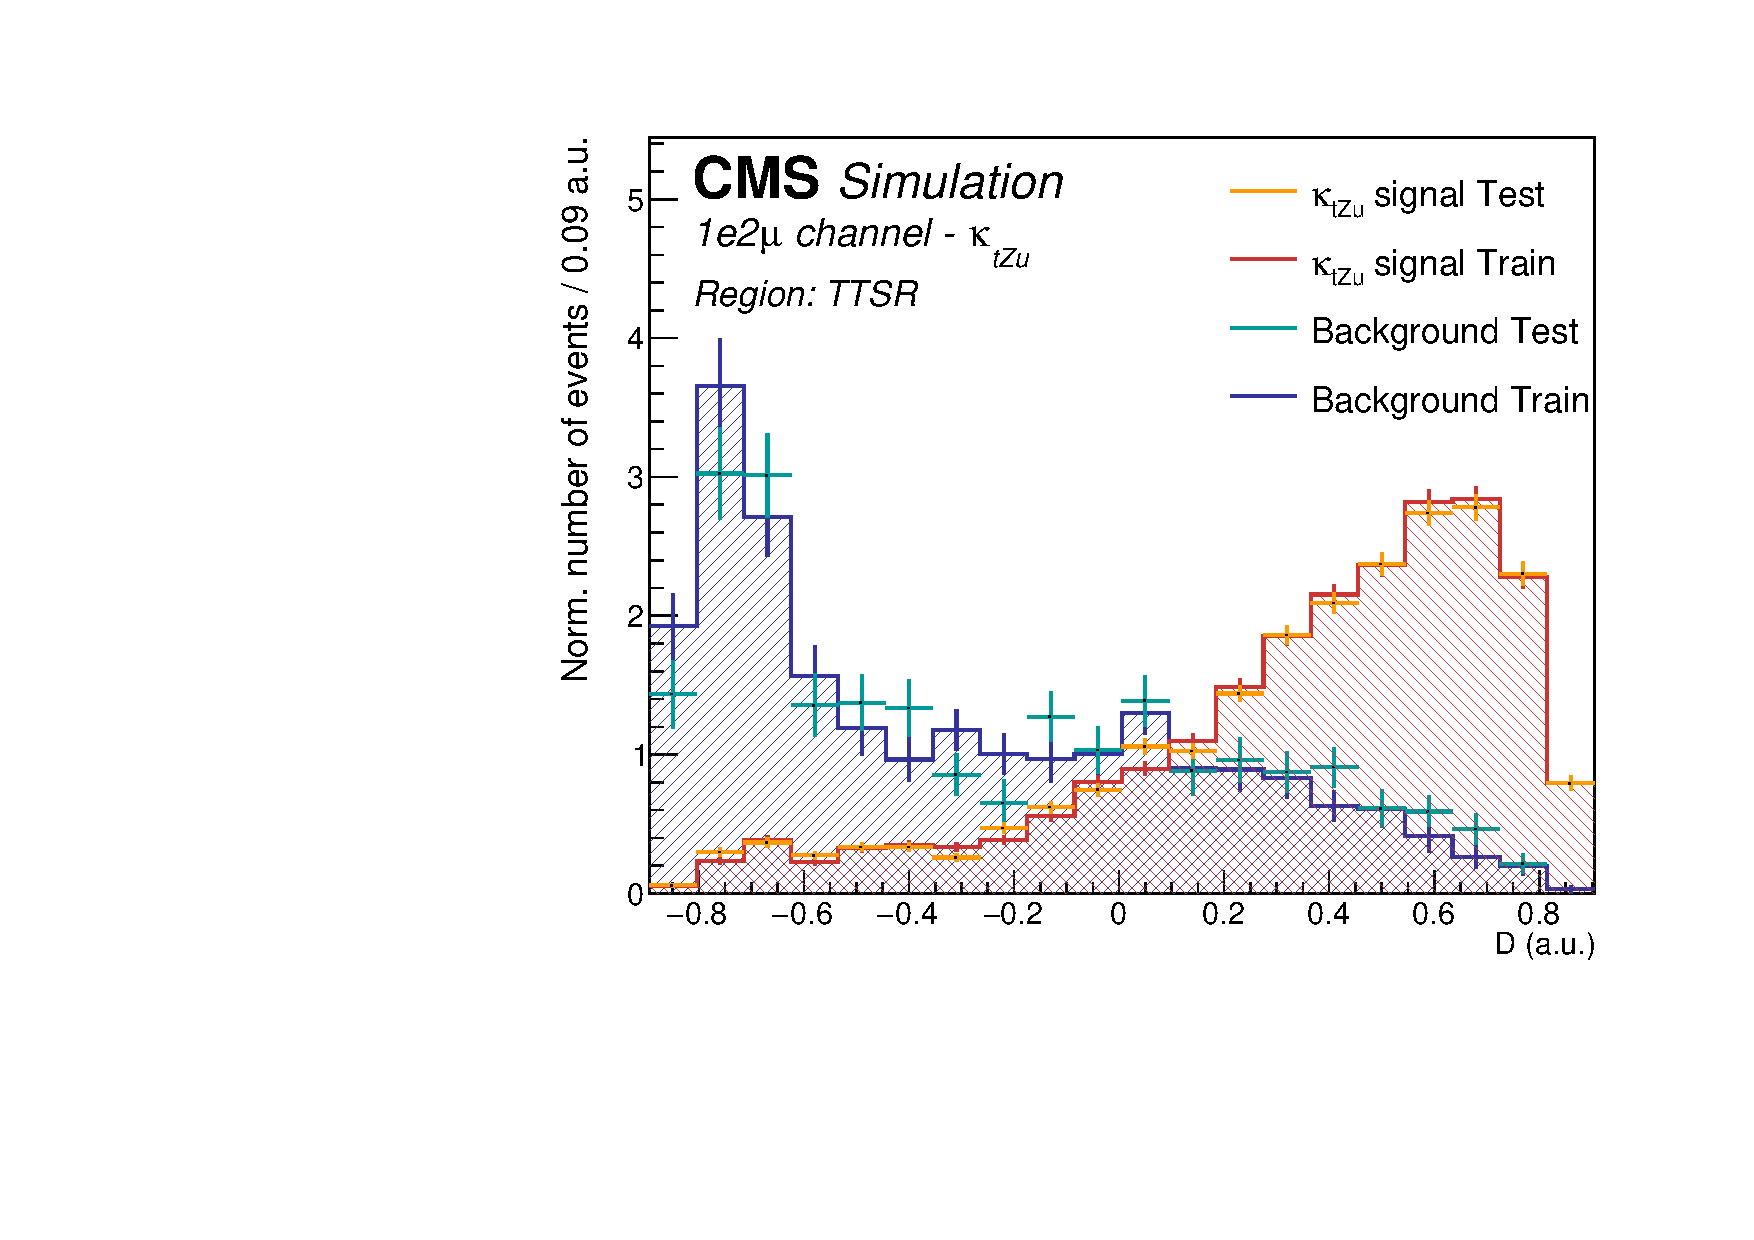
\includegraphics[width=0.49\linewidth]{6_Search/Figures/PlotsTechnics/SigVsBkgTestZuttoppairuue}
	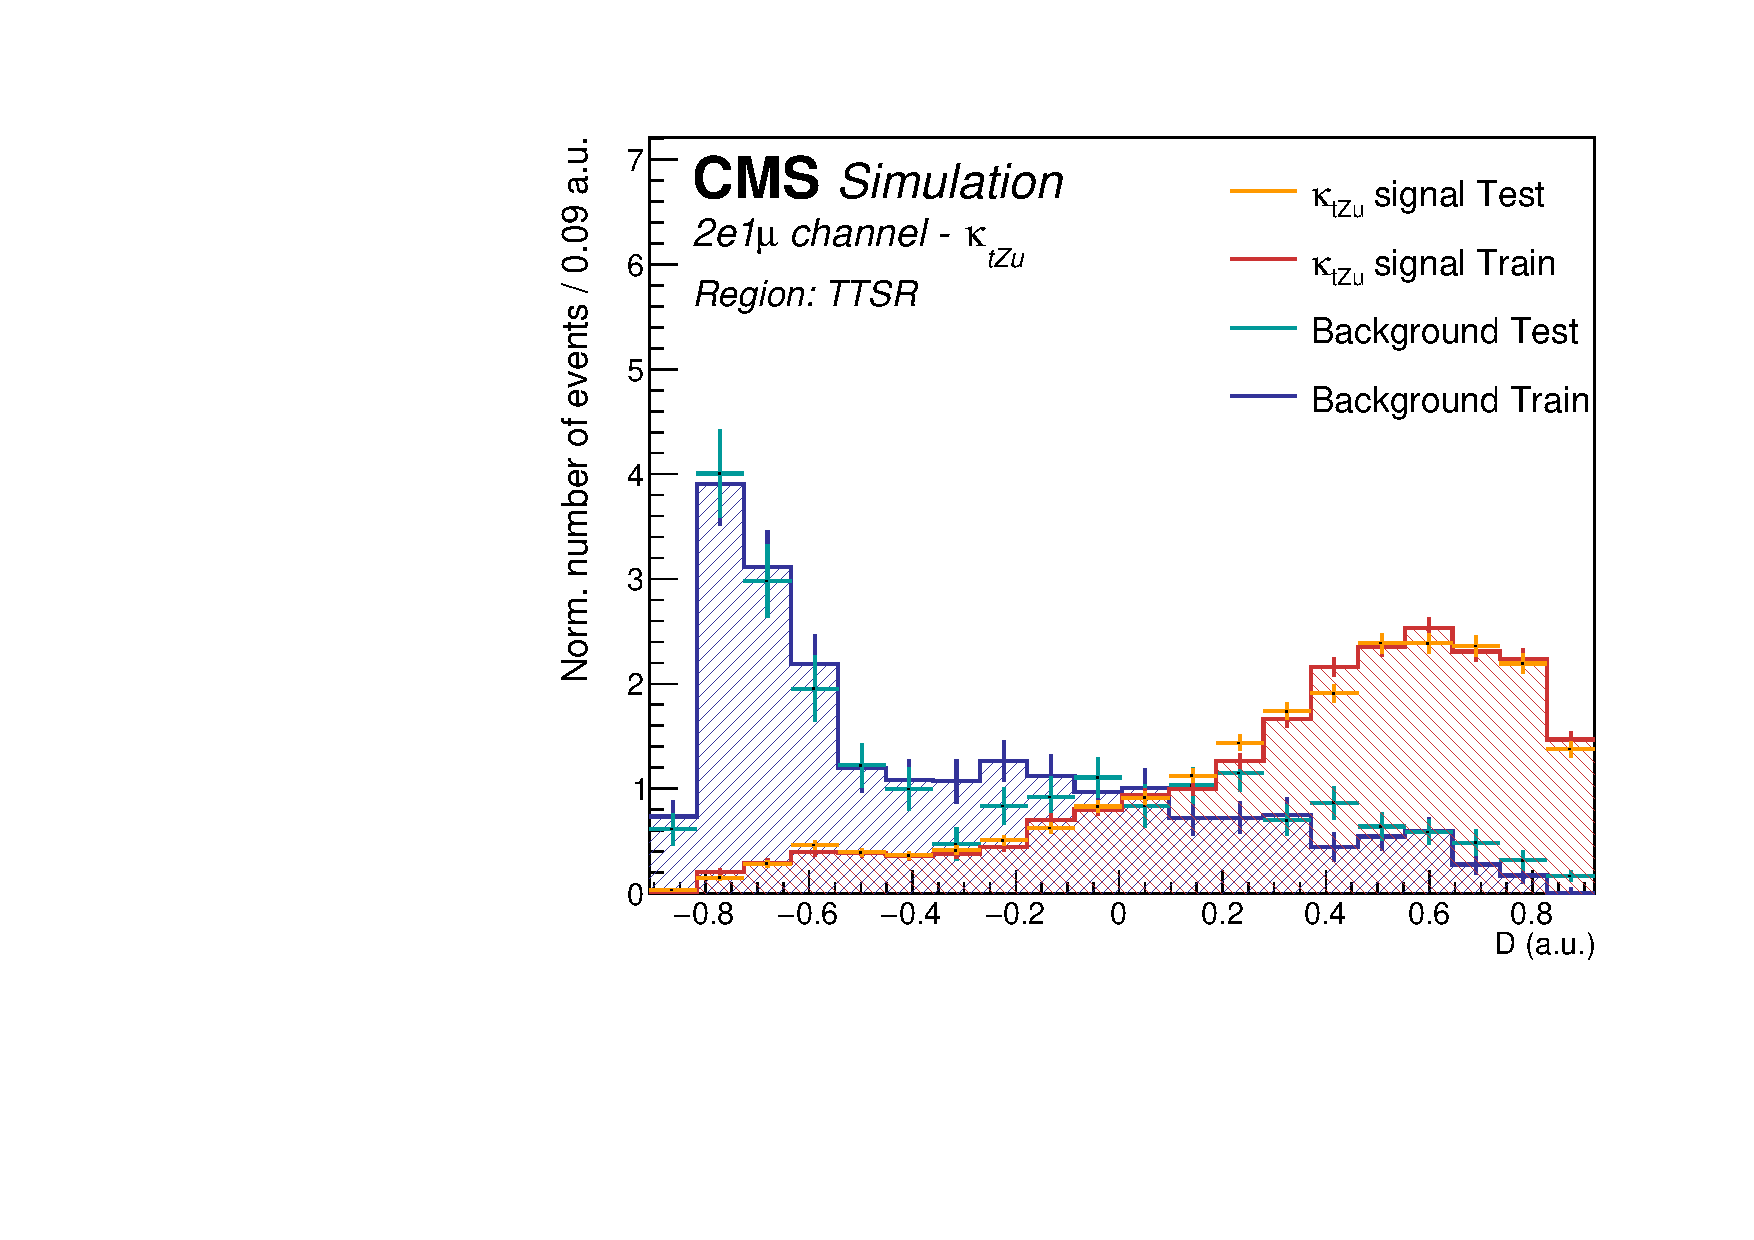
\includegraphics[width=0.49\linewidth]{6_Search/Figures/PlotsTechnics/SigVsBkgTestZuttoppaireeu}
	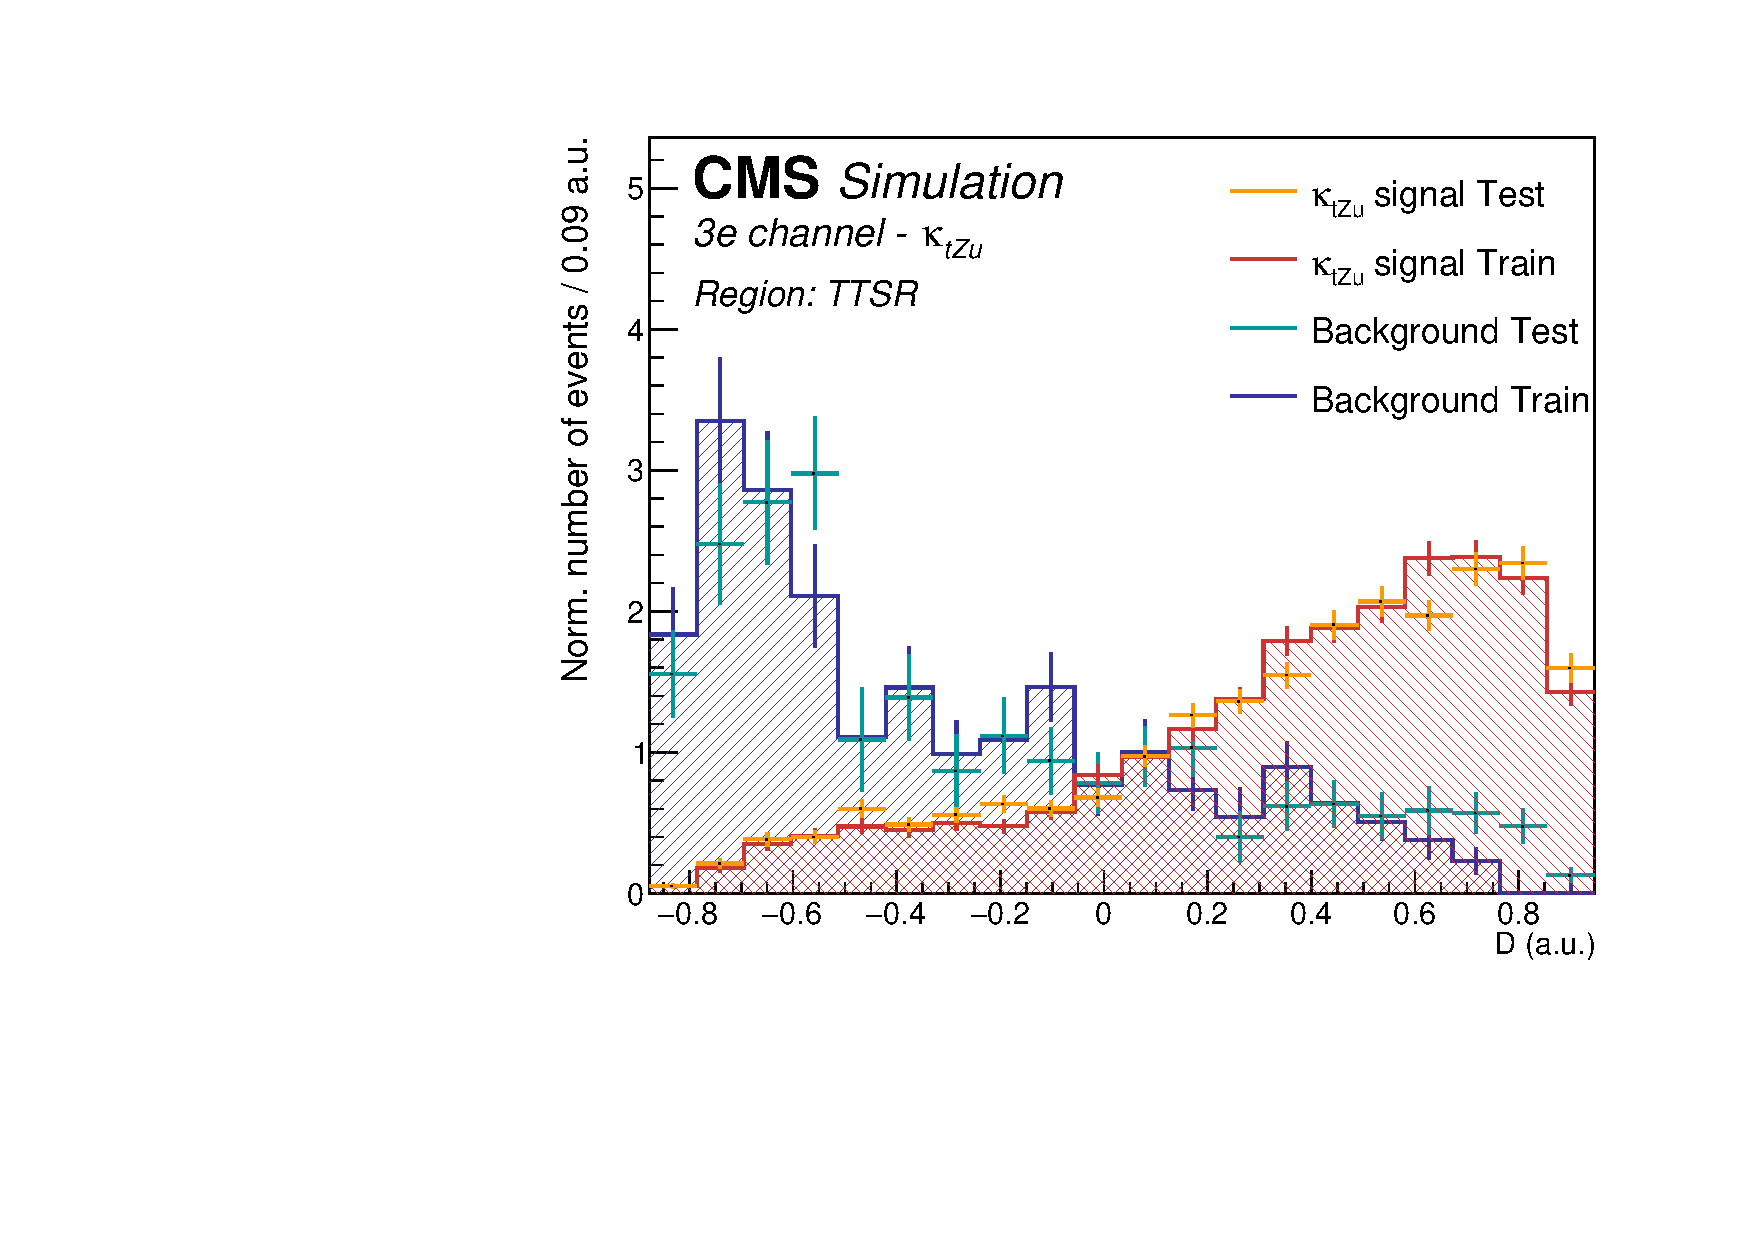
\includegraphics[width=0.49\linewidth]{6_Search/Figures/PlotsTechnics/SigVsBkgTestZuttoppaireee}
	\caption{The normalised distributions of the resulting  multivariate discriminators D in the \TTSR, for the \Zut\ signal. For the \mumumu\ (left,top), \emumu\ (right,top), \eemu\ (left, bottom) and \eee\ (right,bottom) three-lepton channel.}
	\label{fig:sigvsbkgtestzuttoppair}
\end{figure}


\clearpage	
\subsection{BDT training in the \STSR\ for the \Zct\ interaction}
\label{sec:BDTSTSRZCT}
The input variables used to create the multivariate discriminator in the \STSR\ for the \Zct\ interaction are shown in \fig{fig:singletopZctnormalized}. In analogy to the training for the \Zut\ vertex in the \STSR\ (\Sec{sec:BDTSTSRZUT}), the training is performed with the single top quark FCNC signal only. The single top quark FCNC  signal signature is similar to that of the signature expected from the \Zut\ interaction and therefore most of the same variables discussed in \Sec{sec:BDTSTSRZUT} are used. For the charm coupling, both quark and anti-quarks responsible for the production of the single top quark FCNC process, are sea quarks. For this reason no charge asymmetry is expected, and the variables related to the charge asymmetry are left out.
 The most important variables in this region for the \Zct\ interaction,  are the invariant mass of all leptons,  followed by the CSVv2 discriminator of the jet with the highest \pt, and the invariant mass of the \PW\ lepton and \SM\ b jet system. The distributions for the other three-lepton channels are given in \App{app:BDTcorrZctSingle}.
 
 
The correlations between the different input variables are given in \fig{fig:correlationsigzctsingletop}. These correlations are in general small, but vary from zero to $\sim 55\%$.
The resulting multivariate discriminator D is shown in \fig{fig:sigvsbkgtestzctsingletop} for all three-lepton channels. In these plots one can observe that there is a clear discrimination between the FCNC single top quark signal and the backgrounds. Furthermore, the procedure is investigated by cross checking the distribution from the training sample with an independent testing sample. As can be seen in the distributions, these samples agree with eachother, and only a minor overtraining is observed. The ROC curves for the testing and training samples are shown in \fig{fig:roczctsingletop}, where the testing sample has a slightly worse performance than the training sample. Though a clear discrimination power between signal and background like events is obtained. 

\begin{figure}[htbp]
	\centering
	\includegraphics[width=0.3\linewidth]{6_Search/Figures/PlotsTechnics/SMtopetaZctsingletopuuu_norm}
	\includegraphics[width=0.3\linewidth]{6_Search/Figures/PlotsTechnics/mlbZctsingletopuuu_norm}
	\includegraphics[width=0.3\linewidth]{6_Search/Figures/PlotsTechnics/dPhiWlepbZctsingletopuuu_norm}
	\includegraphics[width=0.3\linewidth]{6_Search/Figures/PlotsTechnics/bdiscCSVv2_jet_0Zctsingletopuuu_norm}	\includegraphics[width=0.3\linewidth]{6_Search/Figures/PlotsTechnics/TotalInvMass_lepZctsingletopuuu_norm}
	\includegraphics[width=0.3\linewidth]{6_Search/Figures/PlotsTechnics/dRZWlepZctsingletopuuu_norm}
	\caption{The normalised distributions of the input variables for reconstructing the multivariate discriminator in the \STSR\ for the \Zct\ vertex for the \mumumu\ channel. The contribution of the \NPL\ background is not included. }
	\label{fig:singletopZctnormalized}
\end{figure}

\begin{figure}[htbp]
	\centering
	\includegraphics[width=0.49\linewidth]{6_Search/Figures/PlotsTechnics/correlationsigZctsingletopuuu}
	\includegraphics[width=0.49\linewidth]{6_Search/Figures/PlotsTechnics/correlationsigZctsingletopuue}
	\includegraphics[width=0.49\linewidth]{6_Search/Figures/PlotsTechnics/correlationsigZctsingletopeeu}
	\includegraphics[width=0.49\linewidth]{6_Search/Figures/PlotsTechnics/correlationsigZctsingletopeee}
	\caption{The correlations between the input variables used to create the multivariate discriminant in the \STSR, for the \Zct\ signal. For the \mumumu\ (left,top), \emumu\ (right,top), \eemu\ (left, bottom) and \eee\ (right,bottom) three-lepton channel.}
	\label{fig:correlationsigzctsingletop}
\end{figure}

\clearpage


\begin{figure}[htbp]
	\centering
	\includegraphics[width=0.49\linewidth]{6_Search/Figures/PlotsTechnics/SigVsBkgTestZctsingletopuuu}
	\includegraphics[width=0.49\linewidth]{6_Search/Figures/PlotsTechnics/SigVsBkgTestZctsingletopuue}
	\includegraphics[width=0.49\linewidth]{6_Search/Figures/PlotsTechnics/SigVsBkgTestZctsingletopeeu}
	\includegraphics[width=0.49\linewidth]{6_Search/Figures/PlotsTechnics/SigVsBkgTestZctsingletopeee}
	\caption{The normalised distributions of the resulting  multivariate discriminators D in the \STSR, for the \Zct\ signal. For the \mumumu\ (left,top), \emumu\ (right,top), \eemu\ (left, bottom) and \eee\ (right,bottom) three-lepton channel.}
	\label{fig:sigvsbkgtestzctsingletop}
\end{figure}




\clearpage
\subsection{BDT training in the \TTSR\ for the \Zct\ interaction}
\label{sec:BDTTTSRZCT}
The training in this region for the \Zct\ interaction is performed by looking at both FCNC signal contributions. The discriminating variables used for training are shown in \fig{fig:toppairZctnormalized}. Most of the variables are the same as the ones for the \Zut\ interaction, described in \Sec{sec:BDTTTSRZUT}, since a similar signature is expected. The most important addition is the CSVv2 discriminator value of the FCNC jet. Since here, the FCNC jet is expected to be a charm quark jet, this jet is expected to have a high CSVv2 discriminator value.  One can observe that in the FCNC signal distribution, there is a small bump at the value 0.8, whereas the background distribution goes down towards higher discriminator values.

The most important input variables for this region, are the invariant mass of the \PW\ lepton and the \SM\ b jet system,  the invariant mass of the FCNC top quark and the reconstructed \PZ\ boson mass. The distributions for the other three-lepton channels are given in \App{app:BDTcorrZctTop}. The correlations between the input  variables are shown in \fig{fig:correlationsigzcttoppaier}. These are in general small, but vary from zero to 55\% correlation. 
\begin{figure}[htbp]
	\centering
	\includegraphics[width=0.25\linewidth]{6_Search/Figures/PlotsTechnics/mlbZcttoppairuuu_norm}
	\includegraphics[width=0.25\linewidth]{6_Search/Figures/PlotsTechnics/Zboson_MZcttoppairuuu_norm}
	\includegraphics[width=0.25\linewidth]{6_Search/Figures/PlotsTechnics/dPhiZWlepZcttoppairuuu_norm}
	\includegraphics[width=0.25\linewidth]{6_Search/Figures/PlotsTechnics/dRWlepbZcttoppairuuu_norm}
	\includegraphics[width=0.25\linewidth]{6_Search/Figures/PlotsTechnics/NJets_CSVv2MZcttoppairuuu_norm}
	\includegraphics[width=0.25\linewidth]{6_Search/Figures/PlotsTechnics/FCNCtop_MZcttoppairuuu_norm}
	\includegraphics[width=0.25\linewidth]{6_Search/Figures/PlotsTechnics/dRZcZcttoppairuuu_norm}
	\includegraphics[width=0.25\linewidth]{6_Search/Figures/PlotsTechnics/dRSMjetLightjetZcttoppairuuu_norm}
	\includegraphics[width=0.25\linewidth]{6_Search/Figures/PlotsTechnics/TotalInvMassZcttoppairuuu_norm}
	\includegraphics[width=0.25\linewidth]{6_Search/Figures/PlotsTechnics/dRZWlepZcttoppairuuu_norm}
	\includegraphics[width=0.25\linewidth]{6_Search/Figures/PlotsTechnics/Bdis_LightjetZcttoppairuuu_norm}
	\includegraphics[width=0.25\linewidth]{6_Search/Figures/PlotsTechnics/dRZbZcttoppairuuu_norm}
	\caption{The normalised distributions of the input variables for reconstructing the multivariate discriminator in the \TTSR\ for the \Zct\ vertex, in the \mumumu\ channel.  The contribution of the \NPL\ background is not included.}
	\label{fig:toppairZctnormalized}
\end{figure}

\begin{figure}[htbp]
	\centering
	\includegraphics[width=0.49\linewidth]{6_Search/Figures/PlotsTechnics/correlationsigZcttoppairuuu}
	\includegraphics[width=0.49\linewidth]{6_Search/Figures/PlotsTechnics/correlationsigZcttoppairuue}
	\includegraphics[width=0.49\linewidth]{6_Search/Figures/PlotsTechnics/correlationsigZcttoppaireeu}
	\includegraphics[width=0.49\linewidth]{6_Search/Figures/PlotsTechnics/correlationsigZcttoppaireee}
	\caption{The correlations between the input variables used to create the multivariate discriminant in the \TTSR, for the \Zct\ signal. For the \mumumu\ (left,top), \emumu\ (right,top), \eemu\ (left, bottom) and \eee\ (right,bottom) three-lepton channel.}
	\label{fig:correlationsigzcttoppaier}
\end{figure}

\clearpage

The resulting multivariate discriminator D is shown in \fig{fig:sigvsbkgtestzcttoppaire} for all three-lepton channels. In these plots one can see that there is a clear discrimination between the FCNC single top quark signal and the backgrounds. Furthermore, the distribution from the training sample is compared with an independent testing sample, and  agree with eachother. A small overtraining is observed in the \eee\ channel due to its low number of events. The ROC curves are shown in \fig{fig:roczcttoppair} and show a slightly worse performance for the testing sample, while keeping its separation power. 
\begin{figure}[htbp]
	\centering
	\includegraphics[width=0.49\linewidth]{6_Search/Figures/PlotsTechnics/SigVsBkgTestZcttoppairuuu}
	\includegraphics[width=0.49\linewidth]{6_Search/Figures/PlotsTechnics/SigVsBkgTestZcttoppairuue}
	\includegraphics[width=0.49\linewidth]{6_Search/Figures/PlotsTechnics/SigVsBkgTestZcttoppaireeu}
	\includegraphics[width=0.49\linewidth]{6_Search/Figures/PlotsTechnics/SigVsBkgTestZcttoppaireee}
	\caption{The normalised distributions of the resulting  multivariate discriminators D in the \TTSR, for the \Zct\ signal. For the \mumumu\ (left,top), \emumu\ (right,top), \eemu\ (left, bottom) and \eee\ (right,bottom) three-lepton channel.}
	\label{fig:sigvsbkgtestzcttoppaire}
\end{figure}

\clearpage

\section{Transverse mass in \WZCR}
\label{sec:mtw}
The \WZCR\ is used to estimate the contribution from \WZ+jets and \NPL\ background. This region is constructed such that the contribution of the \WZ+jets process is enhanced with respect to the other backgrounds entering the analysis In this region t, a fit is performed on the transverse mass distribution of the \PW\ boson. For the\WZ+jets background, a real \PW\ boson is expected, and the distribution will peak at the mass of the \PW\ boson. For the \NPL\ background, there is no reason for the distribution to peak at the mass of the \PW\ boson. Since the not prompt-leptons in general tend towards lower \pt\ values, their resulting distribution will peak a zero and decrease towards higher values of $m_{\mathrm{T}}(\PW)$.  The normalised distributions are shown in \fig{fig:mtwnorm} for all three-lepton channels. % The sum of the lepton channels is shown in \fig{fig:mtwallnorm}. 
\begin{figure}[htbp]
	\centering
	\includegraphics[width=0.49\linewidth]{6_Search/Figures/MTWnormalised/MTW_uuu_Normalized}
	\includegraphics[width=0.49\linewidth]{6_Search/Figures/MTWnormalised/MTW_uue_Normalized}
	\includegraphics[width=0.49\linewidth]{6_Search/Figures/MTWnormalised/MTW_eeu_Normalized}
	\includegraphics[width=0.49\linewidth]{6_Search/Figures/MTWnormalised/MTW_eee_Normalized}
	\caption{The normalised distribution of the transverse mass of the W boson in the \WZCR, before the fit. Left: \mumumu, left-middle: \emumu, right-middle: \eemu, and right: \eee\ lepton channel.  }
	\label{fig:mtwnorm}
\end{figure}
%\begin{figure}[htbp]
%	\centering
%	\includegraphics[width=0.49\linewidth]{6_Search/Figures/MTWnormalised/MTW_all_Normalized}
%	\caption{The normalised distribution of the transverse mass of the W boson in the \WZCR, before the fit. All different lepton channels together. }
%	\label{fig:mtwallnorm}
%\end{figure}

\newpage
\section{Systematic uncertainties}
\label{sec:sys}
The systematic uncertainties entering the analysis are coming from different sources. The experimental uncertainties arise from the reconstruction of the objects and are discussed in \Sec{sec:PhysicsObject}. These influence the number of events passing the selection, so-called normalisation uncertainties, and/or the relative occupancies of the distributions, so-called shape
 uncertainties. The normalisation uncertainties coming from reconstruction include the uncertainty of 2.5\% on the measured integrated luminosity and the efficiency of the trigger logic used for the analysis which has a 1\% (5\%) uncertainty on the 
 \mumumu\ and \emumu\ (\eemu\ and \eee) channels. The  pileup distribution is calculated via the minimum bias cross section which has a 4.6\% uncertainty. This uncertainty results in a systematic shift in the pileup distribution and its shape effect is estimated by recalculating the pileup distribution for each variation of the minimum bias cross section. The shape uncertainties also include the uncertainties coming from the applied lepton scale factors. Their systematic uncertainty originates from three sources: identification, isolation and tracking.  The uncertainties arising from jet energy corrections require a recalculation of all jet related kinematic observables and its effect is propagated to the missing transverse energy.  The reweighting of the CSVv2 discriminant is also a source of uncertainty. There are three sources of uncertainty contributing to the measurement of the b-tag related scale factors: statistical uncertainties, jet energy scale and the purity of the sample. These result in eight uncorrelated contributions. 
 
 Since the \NPL\ sample is artificially made from data by inverting the isolation of the third lepton. Its effect has to be estimated. The shape uncertainty for the \NPL\ processes is obtained by varying the isolation inversion with respect to relative isolation value for the tight lepton identification and the relative isolation for  the loose lepton identification for electrons and muons at the same time. This found to have negligible effect. Changing the value of the relative isolation has found to have a negligible effect on the shape of the relative distribution occupancies of the \NPL\ background. The uncertainty on the normalisation of the overall \NPL\ yield is taken as 50\% in accordance with the \SM\ \tZq\ search~\cite{CMS-PAS-TOP-16-020}.
 
 The uncertainty on the expected yield of the simulated backgrounds is taken to be 30\% of the yield such that it covers all uncertainties at next to leading order accuracy. Theory uncertainties  originating from the modelling of the main backgrounds are estimated to account for the effect on the shape of the distributions from the choice of parton density functions, and renormalization (\muR) and factorization (\muF) scales. The effect of the  renormalization (\muR) and factorization (\muF) scales is estimated by varying each independently ($\muR\uparrow$, $\muR\downarrow$, $\muF\uparrow$, or $\muF\downarrow $) and correlated up and down  ($\muR\uparrow\muF\uparrow$ or $\muR\downarrow\muF\downarrow $) by a factor of two. The envelope of these variations is used as an uncertainty. The uncertainties coming from the parton density functions  used for simulation are estimated using the PDF4LHC recipe~\cite{Ball:2017nwa}, which combines the MMHT14, CT14, and NNPDF3.0 PDF sets. The theory uncertainties are considered for the main backgrounds coming from simulation: \WZ+jets, \ZZ+jets, \ttZ, and \tZq. This is found to have a negligible effect.

 The way the uncertainties are treated as nuisance parameters is summarized in \tab{tab:nuis}. The effect of systematic uncertainties that are treated as shape uncertainties is shown in \Sec{sec:MTW} and \Sec{sec:BDTsys} . \todo{INCLUDE EFFECT PDF AND FACT/RENO}

\begin{table}[htbp]
	\centering
	\caption{Uncertainties used in this analysis. The column labelled type represents how the uncertainty is treated for the fit.}
	\begin{tabular}{ccc}
		\toprule
		Source & Systematic input & Type \\ 
		\midrule 
		nonprompt muon norm. & 50\% & normalisation \\ 
		 
		nonprompt electron norm. & 50\% & normalisation \\ 
		 
		background \ttZ\ norm. & 30\% & normalisation \\ 
		 
		background \WZ\ norm. & 30\% & normalisation \\ 
		 
		background \tZq\ norm. & 30\% & normalisation \\ 
		 
		background \ZZ\ norm.& 30\% & normalisation \\ 
		 
		background other MC norm. & 30\% & normalisation \\ 
		 
		trigger & 1\% (5\%) & normalisation \\ 
		 
		lepton identification  & $\pm \sigma(p_{T},\eta)$ & shape \\ 
		 
		JES & $\pm \sigma(p_{T},\eta)$ & shape \\ 
		 
		JER & $\pm \sigma(p_{T},\eta)$ &  shape \\ 
		 
		b-tagging & $\pm \sigma(p_{T},\eta)$ & shape \\ 
		 
		pileup\ & $\pm \sigma$ of min. bias cross section &  shape \\ 
		 
		PDF & PDF4LHC recipe &  shape   \\ 
		 
		luminosity & 2.5\% & normalisation \\ 
		 
		renorm. and fact. scales & varying indep. and corr. &  shape \\ 
		\bottomrule
	\end{tabular} 
	\label{tab:nuis}
\end{table}
\clearpage
\subsection{Effect of systematic uncertainties in \WZCR}
\label{sec:MTW}
The effect of the systematic uncertainties influencing the shape of the distribution of the transverse mass of the \PW\ boson in the \WZCR is shown in this section for the \WZ+jet process by varying each source of uncertainty individually within its uncertainty range.  The uncertainties due to pileup and lepton scale factors, shown in \fig{fig:shiftMTW1}, have the smallest effect on the distribution. The uncertainty on the pileup distribution is clearly influencing the shape of the distribution, while the lepton identification uncertainties are more affecting the normalisation of the whole distribution. 
\begin{figure}[htbp] 
	\centering 
	\subbottom[Pileup uncertainty]{
	    \includegraphics[width=0.3\linewidth]{6_Search/Figures/SystematicEffect/MTWsys/MWT_pileupBKG}
    }
    \subbottom[Electron identification  uncertainty]{
    	\includegraphics[width=0.3\linewidth]{6_Search/Figures/SystematicEffect/MTWsys/MWT_electronBKG}
    }
    \subbottom[Muon identification uncertainty]{
    	\includegraphics[width=0.3\linewidth]{6_Search/Figures/SystematicEffect/MTWsys/MWT_muonBKG}
    }
	\caption{Distribution of the nominal values and shift due to the experimental systematic uncertainties for the transverse mass of the \PW\ boson in the \WZCR\ for the \WZ+jets process. All lepton channels summed.}
\label{fig:shiftMTW1}
\end{figure}

The effect of the uncertainties arising from the jet energy corrections, shown in \fig{fig:shiftMTW3}),  have the largest effect on the shape of the distribution. The jet energy scale has the most influence on the distribution, affecting both its normalisation and shape. This is due to the fact that the missing transverse energy, which is used for constructing the transverse mass of the \PW\ boson, is influenced by the change in jet energy. Still, for the bulk of the distribution, this effect stays within a 10\% margin.
\begin{figure}[htbp] 
	\centering 
	\subbottom[Jet energy scale uncertainty]{
		\includegraphics[width=0.3\linewidth]{6_Search/Figures/SystematicEffect/MTWsys/MTW_JESBKG}
	}
	\subbottom[Jet energy resolution uncertainty]{
		\includegraphics[width=0.3\linewidth]{6_Search/Figures/SystematicEffect/MTWsys/MTW_JERBKG}
	}
	\caption{Distribution of the nominal values and shift due to the experimental systematic uncertainties for the transverse mass of the \PW\ boson in the \WZCR\ for the \WZ+jets process. All lepton channels summed.}
	\label{fig:shiftMTW3}
\end{figure}

The uncertainties due to b-tagging are shown in \fig{fig:shiftMTW2}. The uncertainty due to purity of heavy flavour jets has the largest contribution and stays within 10\% of the nominal shape. This is due to the fact that events are migrating in and out of the \WZCR, based on the presence of b jets. All The uncertainties due to b-tagging uncertainties are not having an impact on the shape of the distribution since no b-tag information is used to construct the transverse mass of the \PW\ boson.
\begin{figure}[htbp] 
	\centering 
	\subbottom[CSVv2: cf uncertainty~(1)]{
		\includegraphics[width=0.3\linewidth]{6_Search/Figures/SystematicEffect/MTWsys/MWT_btagSF_cferr1BKG}
	}
    \subbottom[CSVv2: cf uncertainty~(2)]{
    	\includegraphics[width=0.3\linewidth]{6_Search/Figures/SystematicEffect/MTWsys/MWT_btagSF_cferr2BKG}
    }
    \subbottom[CSVv2: hf uncertainty]{
     	\includegraphics[width=0.3\linewidth]{6_Search/Figures/SystematicEffect/MTWsys/MWT_btagSF_hfBKG}
    }
    \subbottom[CSVv2: lf uncertainty ]{
    	\includegraphics[width=0.3\linewidth]{6_Search/Figures/SystematicEffect/MTWsys/MWT_btagSF_lfBKG}
    }
    \subbottom[CSVv2: hf statistical uncertainty~(1) ]{
    	\includegraphics[width=0.3\linewidth]{6_Search/Figures/SystematicEffect/MTWsys/MWT_btagSF_hfstats1BKG}
    }
    \subbottom[CSVv2: hf statistical uncertainty~(2) ]{
		\includegraphics[width=0.3\linewidth]{6_Search/Figures/SystematicEffect/MTWsys/MWT_btagSF_hfstats2BKG}
    }
    \subbottom[CSVv2: lf statistical uncertainty~(1) ]{
    	\includegraphics[width=0.3\linewidth]{6_Search/Figures/SystematicEffect/MTWsys/MWT_btagSF_lfstats1BKG}
    }
    \subbottom[CSVv2: lf statistical uncertainty~(2) ]{
		\includegraphics[width=0.3\linewidth]{6_Search/Figures/SystematicEffect/MTWsys/MWT_btagSF_lfstats2BKG}
	}
	\caption{Distribution of the nominal values and shift due to the experimental systematic uncertainties for the transverse mass of the \PW\ boson in the \WZCR\ for the \WZ+jets process. All lepton channels summed.}
\label{fig:shiftMTW2}
\end{figure}


\newpage
In \fig{fig:shiftMTWt}, the effect of the theoretical uncertainties uncertainties on the distribution of the \WZ+jets process is shown. The effect of the choice of factorisation and renormalization scale is shown in \fig{fig:shiftMTWt} (a), while the effect of the knowledge of the parton density functions is shown in \fig{fig:shiftMTWt} (b). These uncertainties have a negligible effect. 
\begin{figure}[htbp] 
	\centering 

\subbottom[Factorisation and renormalization scale uncertainty ]{
	\includegraphics[width=0.32\linewidth]{6_Search/Figures/theorysys/factrenoall}
}
\subbottom[PDF uncertainty ]{
	\includegraphics[width=0.32\linewidth]{6_Search/Figures/theorysys/pdfbdtall}
}
	\caption{Distribution of the nominal values and shift due to  systematic uncertainties for the transverse mass of the \PW\ boson in the \WZCR\ for the \WZ+jets process. All lepton channels summed.}
	\label{fig:shiftMTWt}
\end{figure}


\subsection{Effect of the systematic uncertainties in the signal regions}
\label{sec:BDTsys}
In this section, the effect of the systematic uncertainties on the multivariate discriminator in the signal regions is discussed.  Most systematic uncertainties result in an effect distribution of around 3.5\%. These include the uncertainties due to pileup,  lepton identification, jet energy resolution, the b-tagging, as well as those from theory. The uncertainty arising from the jet energy scale correction has the largest effect on the distribution, and stays within 10\%/. 


\section{Limit setting procedure validation}
\label{sec:val}
The analysis strategy has been established using a blinded strategy. This way, one is sure that there is no bias introduced into the analysis. Through the use of a pseudo dataset, the limit setting procedure has been validated. Signal injection tests for which the signal strength from a pseudo dataset with a pre-set  signal strength is estimated are performed and shown in \fig{fig:plotzut}. From these plots, it is clear that for a data set with a signal strength $\mu= 0.1,\;0.2,\;0.3,\;,0.4$ or $0.5$, the maximum likelihood estimate returns the same values. This validation has been done for both the \Zut\ and \Zct\ interaction.
\begin{figure}[htbp]
	\centering
	 \includegraphics[width=0.49\linewidth]{6_Search/Figures/SignalInjection/plotZut}
	 \includegraphics[width=0.49\linewidth]{6_Search/Figures/SignalInjection/plotZct}
	\caption{The  obtained signal strength with the Maximum Likelihood method is in agreement with the signal strength used to generate the pseudo data set for the \Zut\ (left) and \Zct\ (right) couplings.}
	\label{fig:plotzut}
\end{figure}

Another validation has been done by performing a Maximum Likelihood fit in the \WZCR\ only, considering all lepton channels. This validation has been performed to have a validation for the data driven estimation of the \NPL\ yield. A simultaneous fit of the signal strength of the \NPE, \NPM\ and the \WZ+jets backgrounds is done by using the multi-dimensional fit in \texttt{Higgs} \texttt{Combine} \texttt{Tool}. The maximum likelihood estimator of the \NPM\ yield and the one for the \NPE\ are in agreement with eachother. This is expected since both should represent the same sample. The yield of the \WZ+jets is estimated to be 20\% larger than its initial value, which is within its 30\% rate uncertainty. The resulting signal strengths can then be applied on the distribution of the transverse mass of the \PW\ boson to verify data/MC agreement, as can be seen in \fig{fig:mtwstack}. %Furthermore, a goodness of fit test is performed to quantitatively validate the fit.  The resulting  p-value is 0.3 (see \fig{fig:gof} ), which means that it is unlikely to have a  .

%\begin{figure}[htbp]
%	\centering
%	 \includegraphics[width=0.7\linewidth]{6_Search/Figures/GOF/GOF_1000toys}
%	\caption{Goodness of fit testing in the \WZCR\  with 1000 toys. The likelihood ration is denoted as $\lambda$.}
%	\label{fig:gof}
%\end{figure}

\begin{figure}[htbp]
	\centering
	\includegraphics[width=0.49\linewidth]{6_Search/Figures/InitialFit/vars/wzcontrol_MVA_mWt_uuu_Stack}
	\includegraphics[width=0.49\linewidth]{6_Search/Figures/InitialFit/vars/wzcontrol_MVA_mWt_uue_Stack}
	\includegraphics[width=0.49\linewidth]{6_Search/Figures/InitialFit/vars/wzcontrol_MVA_mWt_eeu_Stack}
	\includegraphics[width=0.49\linewidth]{6_Search/Figures/InitialFit/vars/wzcontrol_MVA_mWt_eee_Stack}
	\caption{Distribution of the transverse mass of the \PW\ boson in the \WZCR\ for the \mumumu\ channel (left, upper), \emumu\ channel (right, upper), \eemu\ channel (left, lower), and 3 electrons channel (right, lower). The uncertainty band does not include theoretical uncertainties.}
	\label{fig:mtwstack}
\end{figure}


\newpage
\section{Results and discussion}
\label{sec:Result}
The limit setting procedure explained in \Sec{sec:Stat} is applied and results are obtained for each three-lepton channel separately as well as their combined results. For both the \Zut\ and \Zct\ coupling, the maximum likelihood estimator of their signal strengths $\hat{\mu}$ is compatible with zero as is shown \fig{fig:mlezut}. One can see that the \eee\ lepton channel has the largest uncertainty. This is due to the fact that this channel is the most influenced by the lack of statistics for this search.
\begin{figure}[htbp]
	\centering
	\includegraphics[width=0.49\linewidth]{6_Search/Figures/MLE/MLEZut.pdf}
	\includegraphics[width=0.49\linewidth]{6_Search/Figures/MLE/MLEZct.pdf}
	\caption{The maximum likelihood estimators for the signal strengths for the \Zut\ vertex (right) and \Zct\ vertex (left) per lepton channel as well as the combination in the \STSR, \TTSR, and all regions combined. }
	\label{fig:mlezut}
\end{figure}

The maximum likelihood estimators for the nuisance parameters $\hat{\theta}$ are shown in \fig{fig:171102zctmle} for the \Zct\ and the \Zut\ interactions. Their values obtained from the signal plus background or background only fits are in agreement with eachother. The transfer factors used to project the event rates from the control regions to the signal regions, have an initial value different than one and have small uncertainties. The normalisation uncertainties on the yields of the simulated backgrounds get constrained by the fit. The nuisance parameters related to the \NPL\ backgrounds get pulled by the fit since their initial normalisation was arbitrary chosen. These have the same tendencies for the fit performed for the \Zut\ and \Zct\ interaction.  %A well known verification of the error coverage for the fit is the pull distribution. For a random variable $x$ following a Gaussian distribution of mean $m$ and width $w$, the pull $g$ is defined as
%\begin{equation}
% g = \frac{x - m}{w},
%\end{equation}
%and follows a standard Gaussian with mean zero and unit width. This property can be applied to our case of parameter estimation due to the central limit theorem~\cite{CDF:AN5776}. The pull distributions are shown in \fig{fig:pulls}. These are peaking at zero with tails going to $\pm2.5$.
%\begin{figure}[htbp]
%	\centering
%	\includegraphics[width=.49\linewidth]{6_Search/Figures/impact/pullsZutwithMC.pdf}
%	\includegraphics[width=.49\linewidth]{6_Search/Figures/impact/pullsZctwithMC.pdf}
%	\caption{Post-fit distribution of the pulls for the \Zut\ (left) and \Zct\ (right) vertex.}
%	\label{fig:pulls}
%\end{figure}

%\newpage
 In \fig{fig:impactsZut1} and \fig{fig:impactsZct1}, one can see again that the nuisance parameters related to the \NPL\ normalisations are shifted with respect to their initial values. This is to be expected since their initial  normalisation is arbitrary. Furthermore, the effect of the uncertainties on the maximum likelihood estimate of the signal strength is shown. The search is limited by lack of data, as can be seen from \fig{fig:exclusionlimitbrcomp} and \fig{fig:exclusionlimitbrfcnczct}. After the limited data statistics, the most important systematic uncertainty are the \ttZ\ normalisation, JES uncertainty and the \NPL\ normalisation uncertainty. 
 
 

\begin{figure}[htbp]
	\centering
%	\includegraphics[width=1.\linewidth]{6_Search/Figures/impact/Document}
	\includegraphics[width=1.\linewidth]{6_Search/Figures/impact/canvas_nuisZct.pdf}
	\includegraphics[width=1.\linewidth]{6_Search/Figures/impact/canvas_nuisZut.pdf}
	\caption{Maximum likelihood estimators for the \Zct\ vertex (up) and \Zut\ vertex (down).}
	\label{fig:171102zctmle}
\end{figure}

\newpage
\begin{figure}[htbp] 
	\centering
	  \includegraphics[page=1,width=1.\linewidth,keepaspectratio]{6_Search/Figures/impact/171122Zut.pdf}
	\caption{The pulls of the most influential  nuisance parameters and the influence of their uncertainty on the maximum likelihood estimation of the signal strength $\hat{r}$ for the \Zut\ vertex, part one.}
	\label{fig:impactsZut1}
\end{figure}


\newpage

\begin{figure}[htbp] 
	\centering
	\includegraphics[page=1,width=1.\linewidth,keepaspectratio]{6_Search/Figures/impact/171122Zct.pdf}
	\caption{The pulls of the most influential nuisance parameters and the influence of their uncertainty on the maximum likelihood estimation of the signal strength $\hat{r}$ for the \Zct\ vertex, part one.}
	\label{fig:impactsZct1}
\end{figure}


%\newpage

\subsection{Postfit distributions}
 The distributions of multivariate discriminating  variables as well as the distribution of the transverse mass of the \PW\ boson are recreated with the maximum likelihood estimations of the nuisance parameters. The resulting distributions are shown in \fig{fig:shapesfitALL}, \fig{fig:shapesfit3mu}, \fig{fig:shapesfit1e2mu}, \fig{fig:shapesfit2e1mu}, and \fig{fig:shapesfit3e}. 
 In the \WZCR\ and \TTSR, the regions where the most events  are entering, there is a clear agreement between data and simulation for all three-lepton channels. In the \STSR, there are some jumps due to the fact that the \NPL\ background is made from a limited data sample and does not have a smooth template to fit. 
\begin{figure}[htbp]
	\centering
	\includegraphics[width=0.49\linewidth]{6_Search/Figures/ZutFit/shapes_fit_s_0_all_error_trial.pdf}
	\includegraphics[width=0.49\linewidth]{6_Search/Figures/ZutFit/shapes_fit_s_3_all_error_trial.pdf}
	\includegraphics[width=0.49\linewidth]{6_Search/Figures/ZutFit/shapes_fit_s_4_all_error_trial.pdf}
	\includegraphics[width=0.49\linewidth]{6_Search/Figures/ZctFit/shapes_fit_s_0_all_error_trial.pdf}
	\includegraphics[width=0.49\linewidth]{6_Search/Figures/ZctFit/shapes_fit_s_3_all_error_trial.pdf}
	\includegraphics[width=0.49\linewidth]{6_Search/Figures/ZctFit/shapes_fit_s_4_all_error_trial.pdf}
	\caption{Post fit distributions for the all lepton channels of the transverse mass of the \PW\ boson in the \WZCR\ (left), the multivariate discriminating variable in the \STSR\ (middle), and the multivariate discriminating variable in the \TTSR\ (right) for the \Zut\ (top) and \Zct\ (bottom) couplings. }
	\label{fig:shapesfitALL}
\end{figure}


\begin{figure}[htbp]
	\centering
	\includegraphics[width=0.49\linewidth]{6_Search/Figures/ZutFit/shapes_fit_s_LepChan_3mu_WZCR_error_trial.pdf}
	\includegraphics[width=0.49\linewidth]{6_Search/Figures/ZutFit/shapes_fit_s_LepChan_3mu_STSR_error_trial.pdf}
	\includegraphics[width=0.49\linewidth]{6_Search/Figures/ZutFit/shapes_fit_s_LepChan_3mu_TTSR_error_trial.pdf}
	\includegraphics[width=0.49\linewidth]{6_Search/Figures/ZctFit/shapes_fit_s_LepChan_3mu_WZCR_error_trial.pdf}
	\includegraphics[width=0.49\linewidth]{6_Search/Figures/ZctFit/shapes_fit_s_LepChan_3mu_STSR_error_trial.pdf}
	\includegraphics[width=0.49\linewidth]{6_Search/Figures/ZctFit/shapes_fit_s_LepChan_3mu_TTSR_error_trial.pdf}
	\caption{Post fit distributions for the \mumumu\ lepton channel of the transverse mass of the \PW\ boson in the \WZCR\ (left), the multivariate discriminating variable in the \STSR\ (middle), and the multivariate discriminating variable in the \TTSR\ (right) for the \Zut\ (top) and \Zct\ (bottom) couplings. }
	\label{fig:shapesfit3mu}
\end{figure}

\newpage
\begin{figure}[htbp]
	\centering
	\includegraphics[width=0.49\linewidth]{6_Search/Figures/ZutFit/shapes_fit_s_LepChan_1e2mu_WZCR_error_trial.pdf}
	\includegraphics[width=0.49\linewidth]{6_Search/Figures/ZutFit/shapes_fit_s_LepChan_1e2mu_STSR_error_trial.pdf}
	\includegraphics[width=0.49\linewidth]{6_Search/Figures/ZutFit/shapes_fit_s_LepChan_1e2mu_TTSR_error_trial.pdf}
	\includegraphics[width=0.49\linewidth]{6_Search/Figures/ZctFit/shapes_fit_s_LepChan_1e2mu_WZCR_error_trial.pdf}
	\includegraphics[width=0.49\linewidth]{6_Search/Figures/ZctFit/shapes_fit_s_LepChan_1e2mu_STSR_error_trial.pdf}
	\includegraphics[width=0.49\linewidth]{6_Search/Figures/ZctFit/shapes_fit_s_LepChan_1e2mu_TTSR_error_trial.pdf}
	\caption{Post fit distributions for the \emumu\ lepton channel of the transverse mass of the \PW\ boson in the \WZCR\ (left), the multivariate discriminating variable in the \STSR\ (middle), and the multivariate discriminating variable in the \TTSR\ (right) for the \Zut\ (top) and \Zct\ (bottom) couplings. }
	\label{fig:shapesfit1e2mu}
\end{figure}

\begin{figure}[htbp]
	\centering
	\includegraphics[width=0.49\linewidth]{6_Search/Figures/ZutFit/shapes_fit_s_LepChan_2e1mu_WZCR_error_trial.pdf}
	\includegraphics[width=0.49\linewidth]{6_Search/Figures/ZutFit/shapes_fit_s_LepChan_2e1mu_STSR_error_trial.pdf}
	\includegraphics[width=0.49\linewidth]{6_Search/Figures/ZutFit/shapes_fit_s_LepChan_2e1mu_TTSR_error_trial.pdf}
	\includegraphics[width=0.49\linewidth]{6_Search/Figures/ZctFit/shapes_fit_s_LepChan_2e1mu_WZCR_error_trial.pdf}
	\includegraphics[width=0.49\linewidth]{6_Search/Figures/ZctFit/shapes_fit_s_LepChan_2e1mu_STSR_error_trial.pdf}
	\includegraphics[width=0.49\linewidth]{6_Search/Figures/ZctFit/shapes_fit_s_LepChan_2e1mu_TTSR_error_trial.pdf}
	\caption{Post fit distributions for the \eemu\ lepton channel of the transverse mass of the \PW\ boson in the \WZCR\ (left), the multivariate discriminating variable in the \STSR\ (middle), and the multivariate discriminating variable in the \TTSR\ (right) for the \Zut\ (top) and \Zct\ (bottom) couplings. }
	\label{fig:shapesfit2e1mu}
\end{figure}

\newpage
\begin{figure}[htbp]
	\centering
	\includegraphics[width=0.49\linewidth]{6_Search/Figures/ZutFit/shapes_fit_s_LepChan_3e_WZCR_error_trial.pdf}
	\includegraphics[width=0.49\linewidth]{6_Search/Figures/ZutFit/shapes_fit_s_LepChan_3e_STSR_error_trial.pdf}
	\includegraphics[width=0.49\linewidth]{6_Search/Figures/ZutFit/shapes_fit_s_LepChan_3e_TTSR_error_trial.pdf}
	\includegraphics[width=0.49\linewidth]{6_Search/Figures/ZctFit/shapes_fit_s_LepChan_3e_WZCR_error_trial.pdf}
	\includegraphics[width=0.49\linewidth]{6_Search/Figures/ZctFit/shapes_fit_s_LepChan_3e_STSR_error_trial.pdf}
	\includegraphics[width=0.49\linewidth]{6_Search/Figures/ZctFit/shapes_fit_s_LepChan_3e_TTSR_error_trial.pdf}
	\caption{Post fit distributions for the \eee\  lepton channel of the transverse mass of the \PW\ boson in the \WZCR\ (left), the multivariate discriminating variable in the \STSR\ (middle), and the multivariate discriminating variable in the \TTSR\ (right) for the \Zut\ (top) and \Zct\ (bottom) couplings. }
	\label{fig:shapesfit3e}
\end{figure}

\clearpage
\subsection{Postfit yields}
\label{sec:postfityields}
In \tab{tab:PYieldSTCR} and \tab{tab:PYieldTTCR}, the  event yields for each process after the global fit for the signal involving a \Zut\ vertex is given for respectively the \STCR\ and \TTCR. All background yields are approximately unchanged and the signal is downscaled with factor of 0.2 with respect to its initial yield. In \tab{tab:PYieldWZCR}, the postfit signal yield is consistent with the other control regions. The background contribution of the \NPL\ process has been doubled, resulting in an agreement between data and simulation. The event yields in the signal regions, \STSR\ and \TTSR, are given in \tab{tab:PYieldSTSR} and \tab{tab:PYieldTTSR} respectively. The contributions of the \WZ+jets and \ttZ+jets backgrounds has risen within their uncertainties, and the contribution of the \NPL\ background has increased, making data agree with simulation. 

  \begin{table}[htbp]
	\centering
	\caption{Event yields in the \STCR, after the global fit for the \Zut\ signal.}
	\begin{tabular} {l c c c c c  }
		\toprule
		Process & all channels & \mumumu\ channel & \emumu\ channel & \eemu\ channel &\eee\ channel  \\
		\midrule
		\NPL\ \ttbar& 25.33 $ \pm $ 3.66 &  9.05 $\pm$ 2.12 & 14.49 $\pm$ 2.72 & 0.40 $\pm$ 0.91 & 1.39 $\pm$ 0.82 \\ 
		\ttZ 		&  0.38 $ \pm $ 0.59 &  0.13 $\pm$ 0.04 &  0.15 $\pm$ 0.59 & 0.04 $\pm$ 0.02 & 0.05 $\pm$ 0.02 \\ 
		\WZ 		&  3.82 $ \pm $ 0.20 &  1.54 $\pm$ 0.03 &  1.18 $\pm$ 0.11 & 0.78 $\pm$ 0.15 & 0.32 $\pm$ 0.03\\ 
		\ZZ 		&  0.38 $ \pm $ 0.05 &  0.20 $\pm$ 0.05 &  0.09 $\pm$ 0.01 & 0.05 $\pm$ 0.01 & 0.04 $\pm$ 0.02\\ 
		Other bkg.	&  2.50 $ \pm $ 0.42 &  0.81 $\pm$ 0.33 &  0.78 $\pm$ 0.09 & 0.81 $\pm$ 0.25 & 0.11 $\pm$ 0.01 \\ 
		\tZq 		&  0.29 $ \pm $ 0.04 &  0.13 $\pm$ 0.03 &  0.08 $\pm$ 0.02 & 0.04 $\pm$ 0.01 & 0.04 $\pm$ 0.01 \B \\ 
%		\hdashline
		\kZut  		&  0.09 $ \pm $ 0.01 &  0.04 $\pm$ 0.01 &  0.03 $\pm$ 0.01 & 0.02 $\pm$ 0.01 & <0.01 $\pm$ <0.01 \T \B\\
		\hdashline
		Data 		& 32 $ \pm $ 3 & 11 $\pm$ 1 & 16 $\pm$ 1 & 2 $\pm$ 1 & 1  $\pm$ 1 \T \\
		Total bkg.	& 33 $ \pm $ 4 & 12 $\pm$ 2 & 17 $\pm$ 3 & 2 $\pm$ 1 & 2  $\pm$ 1 \\
		\bottomrule
	\end{tabular}
	\label{tab:PYieldSTCR}
\end{table}
\begin{table}[htbp]
	\centering
	\caption{Event yields in the \TTCR, after the global fit for the \Zut\ signal. }
	
	\begin{tabular} {l c c c c c }
		\toprule
		Process &   all channels & \mumumu\ channel & \emumu\ channel & \eemu\ channel &\eee\ channel \\
		\midrule
		\NPL\ \ttbar& 28.92 $ \pm $ 3.47 & 14.28 $\pm$ 2.00 &  9.79 $\pm$ 2.32 & 4.45 $\pm$ 1.49 & 0.39 $\pm$ 0.67 \\ 
		\ttZ 		&  2.93 $ \pm $ 0.25 &  1.23 $\pm$ 0.20 &  0.66 $\pm$ 0.10 & 0.56 $\pm$ 0.08 & 0.48 $\pm$ 0.08 \\ 
		\WZ			&  4.71 $ \pm $ 0.43 &  2.01 $\pm$ 0.34 &  1.55 $\pm$ 0.25 & 0.57 $\pm$ 0.08 & 0.58 $\pm$ 0.06 \\ 
		\ZZ 		&  0.36 $ \pm $ 0.04 &  0.15 $\pm$ 0.03 &  0.10 $\pm$ 0.02 & 0.05 $\pm$ 0.01 & 0.06 $\pm$ 0.01 \\ 
		Other bkg. 	&  4.05 $ \pm $ 0.31 &  1.60 $\pm$ 0.15 &  1.36 $\pm$ 0.22 & 0.74 $\pm$ 0.13 & 0.35 $\pm$ 0.08 \\ 
		\tZq 		&  0.79 $ \pm $ 0.07 &  0.38 $\pm$ 0.06 &  0.25 $\pm$ 0.04 & 0.10 $\pm$ 0.01 & 0.06 $\pm$ 0.02 \B\\ 
	%	\hdashline
		\kZut  		&  0.13 $ \pm $ 0.01 &  0.06 $\pm$ 0.01 &  0.04 $\pm$ 0.01 & 0.02 $\pm$ 0.01 & 0.02 $\pm$ <0.01  \T\B\\
		\hdashline
		Data 		& 44 $ \pm $ 3 & 19 $\pm$ 1 & 15 $\pm$ 1 & 6 $\pm$ 1 & 2 $\pm$ 1 \T\\
		Total bkg.	& 42 $ \pm $ 3 & 20 $\pm$ 2 & 14 $\pm$ 2 & 6 $\pm$ 2 & 2 $\pm$ 1\\
		\bottomrule
	\end{tabular}
	\label{tab:PYieldTTCR}
\end{table}
\begin{landscape}
	\vspace*{\fill}
	
	\begin{table}[htbp]
		\centering
		\caption{Event yields in the \TTSR, after the global fit for the \Zut\ FCNC signal.  }	
		\begin{tabular} {l c c c c c}
			\toprule
			Process & all channels & \mumumu\ channel & \emumu\ channel & \eemu\ channel &\eee\ channel \\
			\midrule
			\NPL\ \DY  		& 113.23 $ \pm $  5.31 & 45.59 $\pm$  3.83 & 28.77 $\pm$  2.63 & 17.08 $\pm$ 1.76 & 21.80 $\pm$ 1.89 \\ 
			\ttZ 			&  62.23 $ \pm $  1.23 & 25.11 $\pm$  0.89 & 16.65 $\pm$  0.58 & 12.17 $\pm$ 0.48 &  8.30 $\pm$ 0.39 \\ 
			\WZ 			&  15.70 $ \pm $  0.27 &  6.40 $\pm$  0.20 &  4.39 $\pm$  0.11 &  3.03 $\pm$ 0.12 &  1.87 $\pm$ 0.07 \\ 
			\ZZ 			&   5.49 $ \pm $  0.12 &  2.09 $\pm$  0.08 &  1.87 $\pm$  0.08 & 0.80 $\pm$ 0.03 &  0.73 $\pm$ 0.04 \\ 
			Other bkg. 		&   5.89 $ \pm $  0.44 &  2.21 $\pm$  0.15 &  1.45 $\pm$  0.10 & 1.60 $\pm$ 0.40 &  0.62 $\pm$ 0.06\\ 
			\tZq 			&  18.54 $ \pm $  0.24 &  8.27 $\pm$  0.15 &  4.95 $\pm$  0.10 & 3.21 $\pm$ 0.14 &  2.11 $\pm$ 0.07\\ 
			NPL \ttbar      &   10.93 $ \pm $ 0.54 &  4.94 $\pm$  0.26 &  4.05 $\pm$  0.34 & 1.55 $\pm$ 0.20 &  0.40 $\pm$ 0.25 \B\\
	%		\hdashline
			\kZut  			&   4.66 $ \pm $  0.15 &  1.00 $\pm$  0.12 &  1.26 $\pm$  0.07 & 0.89 $\pm$ 0.06 &  0.60 $\pm$ 0.04 \T\B\\
			\hdashline
			Data 			& 243 $ \pm $ 19 & 107 $\pm$ 11 & 58 $\pm$ 10 & 38 $\pm$ 8 & 40 $\pm$ 8 \T \\
			Total bkg. 	& 232 $ \pm $  4 &  95 $\pm$  4 & 62 $\pm$ 3 & 39 $\pm$ 2 & 36 $\pm$ 2 \\
			\bottomrule
		\end{tabular}
		\label{tab:PYieldTTSR}
	\end{table}
	
	
	\vspace*{\fill}
\end{landscape}
\begin{landscape}	
	\vspace*{\fill}
	
	\begin{table}[htbp]
		\centering
		\caption{Event yields in the \STSR, after the global fit for the \Zut\ FCNC signal. }
		
		\begin{tabular} {l c c c c c   }
			\toprule
			Process &   all channels & \mumumu\ channel & \emumu\ channel & \eemu\ channel &\eee\ channel\\
			\midrule
			\NPL\ \DY    & 80.64  $ \pm $  4.44& 36.55 $ \pm $ 3.20& 25.49 $\pm$ 2.78 & 11.27 $\pm$ 1.09 & 7.33 $\pm$ 0.76 \\ 
			\ttZ         & 3.91 $ \pm $ 0.23 & 1.44 $ \pm $ 0.12   &  0.96 $\pm$ 0.10 &  0.94 $\pm$ 0.15 & 0.57 $\pm$ 0.06\\ 
			\WZ          & 7.79 $ \pm $ 0.15 & 3.28 $ \pm $ 0.07   &  2.32 $\pm$ 0.11 &  1.31 $\pm$ 0.05 & 0.88 $\pm$ 0.04\\ 
			\ZZ 		 & 6.21 $ \pm $ 0.40 & 2.42 $ \pm $ 0.25   &  2.31 $\pm$ 0.30 &  0.78 $\pm$ 0.07 & 0.70 $\pm$ 0.06 \\ 
			Other bkg.   & 1.31 $ \pm $ 0.08 & 0.71 $ \pm $ 0.06   &  0.29 $\pm$ 0.03 &  0.19 $\pm$ 0.03 & 0.11 $\pm$ 0.02 \\ 
			\tZq 		 & 8.92 $ \pm $ 0.27 & 4.05 $ \pm $ 0.21   &  2.31 $\pm$ 0.13 &  1.55 $\pm$ 0.09 & 1.01 $\pm$ 0.05\\ 
			NPL \ttbar   &16.13 $ \pm $ 0.88 & 6.00 $ \pm $ 0.51   &  8.04 $\pm$ 0.59 &  0.09 $\pm$ 0.07 & 2.00 $\pm$ 0.41 \B\\
	%		\hdashline
			\kZut  		 & 2.43 $ \pm $ 0.09 & 0.99 $ \pm $ 0.22   &  0.64 $\pm$ 0.05 &  0.48 $\pm$ 0.04 & 0.31 $\pm$ 0.03 \T\B \\
			\hdashline
			Data         & 138 $ \pm $ 15 & 55 $\pm$ 8 & 47 $\pm$ 7 & 21 $\pm$ 5 & 15 $\pm$ 5 \T\\
			Total bkg.   & 125 $ \pm $  5 & 54 $\pm$ 3 & 42 $\pm$ 3 & 16 $\pm$ 1 & 13 $\pm$ 1 \\
			\bottomrule
		\end{tabular}
		\label{tab:PYieldSTSR}
	\end{table}
	\vspace*{\fill}
\end{landscape}
\begin{landscape}
	\vspace*{\fill}
	\begin{table}[htbp]
		\centering
		\caption{Event yields  in the \WZCR, after the global fit for the \Zut\ signal.  }	
		\begin{tabular} {l c c c c c  }
			\toprule
			Process & all channels & \mumumu\ channel & \emumu\ channel & \eemu\ channel &\eee\ channel \\
			\midrule
			\NPL\ \DY  & 408.84 $ \pm $ 13.11 & 152.48 $\pm$ 8.12 &151.47 $\pm$ 7.97 & 40.80 $\pm$ 4.57 & 64.09 $\pm$ 4.62 \\ 
			\ttZ    	& 10.22 $ \pm $ 0.36  &  4.18 $\pm$  0.25 &  2.63 $\pm$ 0.18 &   2.03 $\pm$ 0.14 &  1.39 $\pm$ 0.12 \\ 
			\WZ 		& 591.52 $ \pm $ 11.22& 247.73 $\pm$ 8.19 &164.23 $\pm$ 6.18 & 112.03 $\pm$ 3.28 & 67.53 $\pm$ 3.15 \\ 
			\ZZ 		& 44.46 $ \pm $ 1.25  & 17.93 $\pm$  0.87 &14.36  $\pm$ 0.77 &   6.80 $\pm$ 0.33 & 5.38 $\pm$ 0.32 \\ 
			Other bkg. 	& 7.40 $ \pm $ 0.47   &  3.54 $\pm$  0.36 &  2.13 $\pm$ 0.29 &   1.02 $\pm$ 0.06 & 0.70 $\pm$ 0.06 \\ 
			\tZq 		& 7.47 $ \pm $ 0.20   &  3.10 $\pm$  0.15 &  2.14 $\pm$ 0.10 &   1.36 $\pm$ 0.05 & 0.86  $\pm$ 0.05 \B \\ 
	%		\hdashline 
			\kZut  		& 2.97 $ \pm $ 0.13   &  1.21 $\pm$  0.10 & 0.80 $\pm$ 0.07 &   0.58 $\pm$ 0.05 & 0.38 $\pm$ 0.03 \T\B\\
			\hdashline
			Data        & 1053 $ \pm $ 345 & 415 $\pm$ 21 & 332 $\pm$ 19 & 168 $\pm$ 14 & 138 $\pm$ 13 \T \\
			Total bkg.  & 1070 $ \pm $ 20 & 429 $\pm$ 13 & 337 $\pm$ 13 & 164 $\pm$ 6 & 140 $\pm$ 7 \\
			\bottomrule
		\end{tabular}
		\label{tab:PYieldWZCR}
	\end{table}
	\vspace*{\fill}
\end{landscape}
\newpage
\section{Limits at 95\% CL}
\label{sec:limits}
\subsection{One dimensional limits}

The limit setting procedure used in this search returns  limits on the signal strength modifier which can be translated to limits on signal cross sections. These limits are translated to a limit on the branching fraction using \eq{eq:BR}. Additionally, the limit on the couplings are extracted using the fact that the cross sections are quadratically dependent on the couplings. In  \fig{fig:exclusionlimitbrfcnczut}, the resulting limits at 95\% CL on the branching fraction and couplings related to the \Zut\ vertex is shown. This observed (expected) limit amounts to $\BR < \BRZuto\: (\BRZut)$ when $\kZut \neq 0$ and $ \kZct = 0$. The expected limit surpasses the expected limit of 2.7$\times 10^{-4}$  of the previous CMS search at a centre-of-mass of 8 \TeV~\cite{Sirunyan:2017kkr}. However, the observed limit of  \BRZuto\ for the \Zut\ interaction does not surpass its observed limit of $2.2\times 10^{-4}$~\cite{Sirunyan:2017kkr}. The ATLAS collaboration has also set limits 95\% CL at a centre-of-mass of 13~\TeV~\cite{ATLAS-CONF-2017-070} with
observed (expected) limits of 1.7$\times 10^{-4}$ (2.4$\times 10^{-4}$) for the \Zut\ coupling. The expected limit presented in this analysis surpasses the expected limit set by ATLAS for the \Zut\ interaction.
 \begin{figure}[htbp]
	\centering
	\includegraphics[width=0.7\linewidth]{6_Search/Figures/ExclusionPlots1D_2017_11_20/ExclusionLimit_BR_FCNC_Zut.pdf}
	\includegraphics[width=0.7\linewidth]{6_Search/Figures/ExclusionPlots1D_2017_10_25/ExclusionLimit_Kappa_FCNC_Zut.pdf}
	\caption{Exclusion limits at 95\% CL on the FCNC branching fractions (left) and couplings (right) as a function of the cross section of the FCNC process,  considering only the \Zut\ vertex. The CMS observed (expected) limit at 95\% CL at a centre-of-mass of 8 \TeV~\cite{Sirunyan:2017kkr} is given with a blue line (dashed line).}
	\label{fig:exclusionlimitbrfcnczut}
\end{figure}

In \fig{fig:exclusionlimitbrcomp} and \tab{tab:ResultsTZU}, the limits for each lepton channel separate as well as their combined limits are shown for the \Zut\ vertex. The lepton channels are in agreement with each other, where the presence of a muon helps pushing the limit further. The \STSR\ is the most sensitive region because of the higher presence of the targeted single top quark signal. Further, one can see that by combining single top quark and top quark pair signals  one gains in sensitivity with 0.005\%.
\begin{table}[htbp]
	\centering
	\caption{Expected limits on the branching fractions at 95\% CL for the tZu coupling~\cite{Sirunyan:2017kkr,ATLAS-CONF-2017-070}.}
	\begin{tabular}{ccccccc}
		\toprule
		& expected & $+2\sigma$ & $+1\sigma$ & $-1\sigma$ & $-2\sigma$ & observed \\ 
		& $\times 10^{-4}$ & $\times 10^{-4}$ & $\times 10^{-4}$ & $\times 10^{-4}$ & $\times 10^{-4}$ & $\times 10^{-4}$ \\
		\midrule
		\mumumu\ &3.2  & 7.4  & 5.0  & 2.1  &1.4  & 5.3  \\ 
	
		\emumu\ & 3.2  & 7.4  & 5.0  & 0.021  & 1.4  & 6.4  \\ 
		
		\eemu\ & 3.6  & 8.4  & 5.6  & 2.3  & 1.6  & 5.6  \\ 
		
		\eee\ & 5.0  & 13  & 8.2  &3.1  & 2.1  & 3.8  \B \\ 
		\hdashline
		\STSR\ only &2.0  & 4.9  & 3.2  & 1.3  & 0.86  & 2.5   \T\\ 
		
		\TTSR\ only & 2.5  & 5.4  & 3.8  & 2.5  & 1.7  & 3.9  \B \\ 
		\hdashline
		combined & 1.5  & 3.3  & 2.3  & 0.97  & 0.68  & 2.4   \T \B\\ 
		\hdashline
		8 \TeV\ CMS (19.7 \fbinv)   &2.7  & -   & 42  & 1.8  & -  & 2.2   \T\B\\
		\hdashline
		13 \TeV\ ATLAS (36 \fbinv)   & 2.4  & -  &   35  &1.7 & -  & 1.7  \T\\
		
		\bottomrule
	\end{tabular} 
	\label{tab:ResultsTZU}
\end{table}
\begin{figure}[htbp]
	\centering
	\includegraphics[width=1.\linewidth]{6_Search/Figures/TOP-17-017_limitsZutStat.pdf}
%	\includegraphics[width=0.49\linewidth]{Figures/TOP-17-017_limitsZct.pdf}
	\caption{Exclusion limits at 95\% CL for each lepton channel and signal region on the FCNC \Zut\ branching fractions considering one non-vanishing coupling at a time. The CMS observed (expected) limit at 95\% CL at a centre-of-mass of 8 \TeV~\cite{Sirunyan:2017kkr} is given with a blue line (dashed line).}	
	\label{fig:exclusionlimitbrcomp}
\end{figure}

\newpage
 In  \fig{fig:exclusionlimitbrfcnczct}, the resulting limits at 95\% CL on the branching fraction and couplings related to the \Zct\ vertex are shown. For this coupling, the observed (expected) limit at 95\% CL is $\BR < \BRZcto\: (\BRZct)$ when $\kZct \neq 0$ and $ \kZut = 0$. The expected limit surpasses the expected limit of  12$\times 10^{-4}$  set by the previous CMS search at a centre-of-mass of 8 \TeV~\cite{Sirunyan:2017kkr}. This also the case for the observed limit, which surpasses the observed limit of 4.9$\times 10^{-4}$ of the previous CMS search~\cite{Sirunyan:2017kkr}. The observed (expected) limit set by the ATLAS collaboration at a centre-of-mass of 13~\TeV~\cite{ATLAS-CONF-2017-070} is 2.3$\times 10^{-2}$ (3.2$\times 10^{-2}$) for the \Zct\ coupling. The expected limit presented in this analysis is in accordance with this limit.
 \begin{figure}[htbp]
 	\centering
 	\includegraphics[width=0.7\linewidth]{6_Search/Figures/ExclusionPlots1D_2017_11_20/ExclusionLimit_BR_FCNC_Zct.pdf}
 	\includegraphics[width=0.7\linewidth]{6_Search/Figures/ExclusionPlots1D_2017_10_25/ExclusionLimit_Kappa_FCNC_Zct.pdf}
 	\caption{Exclusion limits at 95\% CL on the FCNC branching fractions (left) and couplings (right) as a function of the cross section of the FCNC process,  considering only the \Zct\ vertex. The CMS observed (expected) limit at 95\% CL at a centre-of-mass of 8 \TeV~\cite{Sirunyan:2017kkr} is given with a blue line (dashed line).}
 	\label{fig:exclusionlimitbrfcnczct}
 \end{figure}
 

The limits for each lepton channel separate as well as their combined limits are shown for the \Zct\ vertex in  \fig{fig:exclusionlimitbrcompc} and \tab{tab:ResultsTZC}. The lepton channels are in agreement with eachother, and the presence of a muon helps the sensitivity. For the \Zct\ vertex, the \TTSR\ is the most sensitive region  and by combining single top quark and top quark pair signals, one also gains in sensitivity with 0.007\%. 

\begin{table}[htbp]
	\centering
	\caption{Expected limits on the branching fractions at 95\% CL for the \Zct\ coupling~\cite{Sirunyan:2017kkr,ATLAS-CONF-2017-070}.}
	\begin{tabular}{ccccccc}
		\toprule
		& expected & $+2\sigma$ & $+1\sigma$ & $-1\sigma$ & $-2\sigma$ & observed \\ 
			& $\times 10^{-4}$ & $\times 10^{-4}$ & $\times 10^{-4}$ & $\times 10^{-4}$ & $\times 10^{-4}$ & $\times 10^{-4}$ \\
		
		\midrule
		\mumumu\ & 7.0  & 15  & 10  & 4.6  & 3.2  & 12  \\ 
		
		\emumu\ & 7.9  & 18  & 12  & 5.2  & 3.6  & 9.6  \\ 
		
		\eemu\ & 8.9  & 20  & 14  & 5.8  & 4.0  & 9.9  \\ 
		
		\eee\ & 12  & 29  & 19  & 7.5  & 5.0  & 9.5  \B\\ 
		\hdashline
		\STSR\ only & 10  & 20  & 16  & 6.6  & 4.5  & 17  \T \\ 
		
		\TTSR\ only & 4.4  & 9.4  & 6.6  & 2.9  & 2.0  & 4.3  \B \\ 
		\hdashline 
		combined & 3.7  & 8.1  & 5.6  & 2.5  & 1.7  & 4.5  \T\B\\ 
		\hdashline
		8 \TeV\ CMS (19.7 \fbinv)    & 12  & -  &22  & 7.1  & -  & 4.9  \T\B\\
		\hdashline
		13 \TeV\ ATLAS (36 \fbinv)    & 3.2  & -  &4.6  & 2.2 & -  & 2.3  \T\\
		\hline
	\end{tabular} 
	\label{tab:ResultsTZC}
\end{table}
\begin{figure}[htbp]
	\centering
	\includegraphics[width=1.\linewidth]{6_Search/Figures/TOP-17-017_limitsZctStat.pdf}
	%	\includegraphics[width=0.49\linewidth]{Figures/TOP-17-017_limitsZct.pdf}
	\caption{Exclusion limits at 95\% CL for each lepton channel and signal region on the FCNC \Zct\ branching fractions considering one non-vanishing coupling at a time. The CMS observed (expected) limit at 95\% CL at a centre-of-mass of 8~\TeV~\cite{Sirunyan:2017kkr} is given with a blue line (dashed line).}	
	\label{fig:exclusionlimitbrcompc}
\end{figure}


\subsection{Two-dimensional limits}
One can interpolate the one dimensional limits to a scenario where both couplings are non-vanishing. The interpolation is taken from Ref.~\cite{CMS-PAS-TOP-17-003}, where an experimental extrapolation formulae
\begin{equation}
 \kZct =  \kZct^{\mathrm{1D}} \sqrt{1 - \frac{\kZut} {{\kZut}^{\mathrm{1D}}}}, 
\end{equation}
is found from 100 benchmark scenarios. These scenarios are constructed from existing signal samples as
\begin{equation}
	\mathrm{Signal\: yield} = (\kZut)^2 (\mathrm{ST\: tZu \: yield + TT\: tZu \: yield }) + (\kZct)^2 (\mathrm{ST\: tZc \: yield + TT\: tZc \: yield }). 
\end{equation}
The resulting two-dimensional limits are shown in \fig{fig:exclusionlimitbrfcnc}. 
\begin{figure}[htbp]
	\centering
	\includegraphics[width=0.7\linewidth]{6_Search/Figures/ExclusionPlots2D_2017_11_20/ExclusionLimit_BR_FCNC.pdf}
	\includegraphics[width=0.7\linewidth]{6_Search/Figures/ExclusionPlots2D_2017_10_25/ExclusionLimit_Kappa_FCNC.pdf}
	\caption{Two-dimensional limits on the branching fractions (left) and couplings (right) for FCNC interactions involving a tZq vertex.  The CMS observed (expected) limit at 95\% CL at a centre-of-mass of 8~\TeV~\cite{Sirunyan:2017kkr} is given with a blue line (dashed line).}
	\label{fig:exclusionlimitbrfcnc}
\end{figure}




